% \section{Exploración del conjunto de datos PeeringDB} \label{sec:anexo_exploracion_datos_peeringdb}

% A continuación, se presenta una breve exploración del archivo de peeringDB correspondiente a la fecha de 02/01/2024 
% \texttt{peeringdb\_2\_dump\_2024\_02\_01.json}, el cual contiene información pública utilizada para describir la infraestructura de Sistemas Autónomos (ASes), Internet Exchange Points (IXPs) y organizaciones asociadas. \\


% El archivo se encuentra en formato \texttt{JSON} y contiene las siguientes claves principales:
% \begin{verbatim}
% dict_keys(['ixlan', 'ixfac', 'carrierfac', 'netixlan', 'ix', 'net', 
%            'netfac', 'poc', 'api', 'fac', 'carrier', 'org', 
%            'ixpfx', 'as_set', 'campus'])
% \end{verbatim}

% Las tablas más importantes para este estudio son las siguientes :
% \begin{itemize}
%     \item \textbf{net}: Las redes (AS) registradas en PeeringDB, junto con su información  de país, tipo de organización, tráfico e información de peering.
    
%     \item \textbf{ix}: Información general de los Internet Exchange Points (IXPs) con su información de nombre, país, ciudad, organización administradora, etc.

%     \item \textbf{fac}: Representa las instalaciones o centros de datos donde las redes y los IXPs están físicamente presentes. Incluye información geográfica y de estado operativo.
    
%     \item \textbf{netfac}: Relaciona cada red (\textbf{net}) con los centros de datos (\textbf{fac}) en los que tiene presencia.

%     \item \textbf{org}: Contiene información sobre las organizaciones administradoras de redes, IXPs y facilities, como su nombre, país y tipo de entidad.

% \end{itemize}


% \subsection*{Exploración de la tabla \texttt{net}}

% Esta tabla recopila la información disponible en PeeringDB sobre diferentes Sistemas Autónomos presentes en Internet y que se tiene su registro en dicha plataforma. Cada elemento representa un AS y describe atributos como tipo de organización, tráfico, políticas de peering, características de conectividad entre otras. 
% Al transformar esta a un Data Frame, esta contiene \textbf{29,418} filas correspondiente a información sobre diferentes ASes y \textbf{40} columnas correspondiente a atributos de estos.\\

% En primer lugar, se analizaron las columnas y sus tipos de datos, identificando \textbf{6 columnas numéricas}, \textbf{27 categóricas} y \textbf{6 booleanas}.


% \begin{lstlisting}[language=Python, caption={Columnas del conjunto de datos \texttt{net}.}, label={lst:columnas_net}]
% === Columnas numéricas ===
% ['fac_count', 'id', 'ix_count', 'org_id', 'info_prefixes6', 'info_prefixes4']

% === Columnas categóricas ===
% ['status', 'looking_glass', 'route_server', 'netixlan_updated', 'info_ratio', 
%  'status_dashboard', 'rir_status', 'created', 'name_long', 'policy_general', 
%  'website', 'updated', 'info_types', 'rir_status_updated', 'netfac_updated', 
%  'info_traffic', 'policy_locations', 'name', 'info_scope', 'notes', 'policy_url', 
%  'poc_updated', 'info_type', 'social_media', 'policy_contracts', 'aka', 'irr_as_set']

% === Columnas booleanas ===
% ['policy_ratio', 'info_unicast', 'allow_ixp_update', 'info_multicast', 
%  'info_never_via_route_servers', 'info_ipv6']
% \end{lstlisting}


% Tras esta primera exploración, se decidió conservar las columnas categóricas relevantes para el estudio, principalmente aquellas que entregan información sobre políticas de conexión, tráfico y alcance de red. Las categorías identificadas se resumen en la Tabla~\ref{tab:categorias_peeringdb_clara}.


% \begin{table}[H]
% \centering
% \caption{Resumen de las categorías presentes en las columnas categóricas seleccionadas del conjunto \texttt{net} de PeeringDB.}
% \label{tab:categorias_peeringdb_clara}
% \begin{tabularx}{\textwidth}{lX}
% \hline
% \textbf{Columna} & \textbf{Categorías y ejemplos de valores} \\
% \hline

% \texttt{policy\_contracts} (4 categorías) &
% Required, Not Required, Private Only, (vacío). \\

% \texttt{info\_type} (10 categorías) &
% NSP, Content, Non-Profit, Cable/DSL/ISP, Educational/Research, 
% Network Services, Enterprise, Route Server, Route Collector, (vacío). \\

% \texttt{info\_scope} (11 categorías) &
% Global, Europe, North America, Regional, Asia Pacific, South America, 
% Not Disclosed, Australia, Middle East, Africa, (vacío). \\

% \texttt{policy\_locations} (6 categorías) &
% Required – International, Not Required, Preferred, Required – US, Required – EU, (vacío). \\

% \texttt{info\_traffic} (19 categorías) &
% 0–20 Mbps, 20–100 Mbps, 5–10 Gbps, 10–20 Gbps, 100–200 Gbps, 500–1000 Gbps, 
% 1–5 Tbps, 50–100 Tbps, 100+ Tbps, (vacío). \\

% \texttt{info\_types} (9 categorías) &
% NSP, Content, Non-Profit, Cable/DSL/ISP, Educational/Research, 
% Network Services, Enterprise, Route Server, Route Collector. \\

% \texttt{policy\_general} (5 categorías) &
% Restrictive, Open, Selective, No, (vacío). \\

% \texttt{info\_ratio} (7 categorías) &
% Balanced, Heavy Inbound, Heavy Outbound, Mostly Inbound, 
% Mostly Outbound, Not Disclosed, (vacío). \\

% \hline
% \end{tabularx}
% \end{table}



% Posteriormente, se analizó los valores faltantes en las distintas columnas.  
% En el caso de las columnas numéricas, se consideraron faltantes los valores \texttt{NaN} y aquellos igual a cero (Tabla~\ref{tab:faltantes_numericos}).


% \begin{table}[H]
% \centering
% \caption{Porcentaje de valores faltantes o nulos en columnas numéricas del conjunto \texttt{net}.}
% \label{tab:faltantes_numericos}
% \begin{tabular}{lcc}
% \hline
% \textbf{Columna} & \textbf{Faltantes} & \textbf{\% Faltantes} \\
% \hline
% \texttt{fac\_count}       & 17,617 & 59.89 \\
% \texttt{ix\_count}        & 14,077 & 47.85 \\
% \texttt{info\_prefixes6}  & 11,870 & 40.35 \\
% \texttt{info\_prefixes4}  & 9,107  & 30.96 \\
% \texttt{id}               & 0      & 0.00 \\
% \texttt{org\_id}          & 0      & 0.00 \\
% \hline
% \end{tabular}
% \end{table}

% De igual forma para las columnas categóricas s consideraron como faltantes los valores \texttt{NaN} y los string vacios. Los resultados se muestran en la Tabla~\ref{tab:faltantes_categoricas}.

% \begin{table}[H]
% \centering
% \caption{Porcentaje de valores faltantes en las columnas categóricas seleccionadas del conjunto \texttt{net} de PeeringDB.}
% \label{tab:faltantes_categoricas}
% \renewcommand{\arraystretch}{1.2}
% \begin{tabular}{lcc}
% \hline
% \textbf{Columna} & \textbf{Faltantes} & \textbf{\% Faltantes} \\
% \hline
% \texttt{info\_traffic}      & 12,047 & 40.95 \\
% \texttt{info\_type}         & 8,439  & 28.69 \\
% \texttt{policy\_contracts}  & 1,462  & 4.97  \\
% \texttt{policy\_general}    & 1,352  & 4.60  \\
% \texttt{policy\_locations}  & 1,353  & 4.60  \\
% \texttt{info\_ratio}        & 663    & 2.25  \\
% \texttt{info\_scope}        & 370    & 1.26  \\
% \texttt{info\_types}        & 0      & 0.00  \\
% \hline
% \end{tabular}
% \end{table}


% Finalmente, la Tabla~\ref{tab:categorias_categoricas} resume las columnas categóricas seleccionadas junto con el número de categorías únicas y algunos ejemplos representativos.  
% Este resumen permite identificar de forma clara la diversidad de información contenida en PeeringDB y la relevancia de cada atributo para su posterior uso en la construcción de modelos basados en grafos.


% \begin{table}[H]
% \centering
% \caption{Resumen de columnas categóricas y número de categorías únicas en PeeringDB.}
% \label{tab:categorias_categoricas}
% \begin{tabular}{lcc}
% \hline
% \textbf{Columna} & \textbf{Categorías únicas} & \textbf{Ejemplos de categorías} \\
% \hline
% policy\_general & 5 & Open, Selective, Restrictive, No \\
% info\_type & 10 & NSP, Content, Non-Profit, Enterprise, Route Server \\
% info\_scope & 11 & Global, Europe, North America, Regional, Asia Pacific \\
% policy\_locations & 6 & Required - US, Required - EU, Not Required \\
% info\_traffic & 18 & 1-5Gbps, 100-200Gbps, 10-20Tbps, 0-20Mbps \\
% info\_ratio & 7 & Balanced, Heavy Inbound, Mostly Outbound \\
% \hline
% \end{tabular}
% \end{table}





% A continuación, algunas figuras para entender los datos.\\





% \begin{figure}[H]
%     \centering
%     % === 1ra fila ===
%     \begin{subfigure}[b]{0.48\textwidth}
%         \centering
%         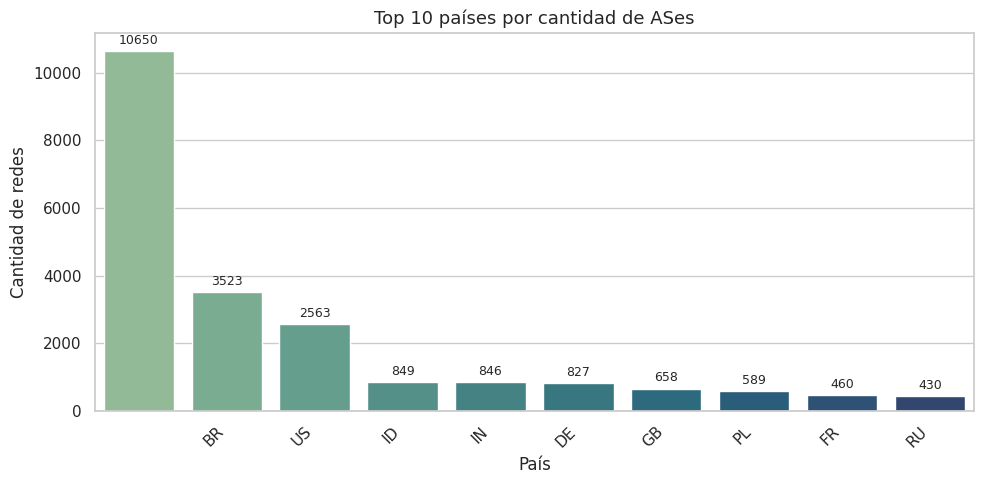
\includegraphics[width=\textwidth]{img/anexoPeeringDB/Top_10_países_por_cantidad_de_ASes.png}
%         \caption{Top 10 países con mayor cantidad de ASes registrados en PeeringDB.}
%         \label{fig:Top_10_países_por_cantidad_de_ASes}
%     \end{subfigure}
%     \hfill
%     \begin{subfigure}[b]{0.48\textwidth}
%         \centering
%         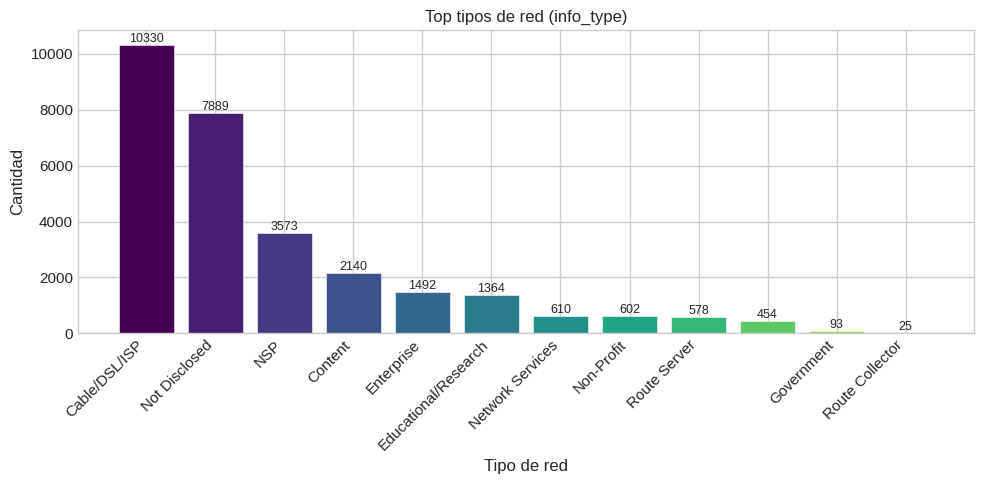
\includegraphics[width=\textwidth]{img/anexoPeeringDB/Top_tipos_de_red_info_type.png}
%         \caption{Top tipos de red (\texttt{info\_type}) en ASes registrados en PeeringDB.}
%         \label{fig:Top_tipos_de_red_info_type}
%     \end{subfigure}

%     % === 2da fila ===
%     \vspace{5mm}
%     \begin{subfigure}[b]{0.48\textwidth}
%         \centering
%         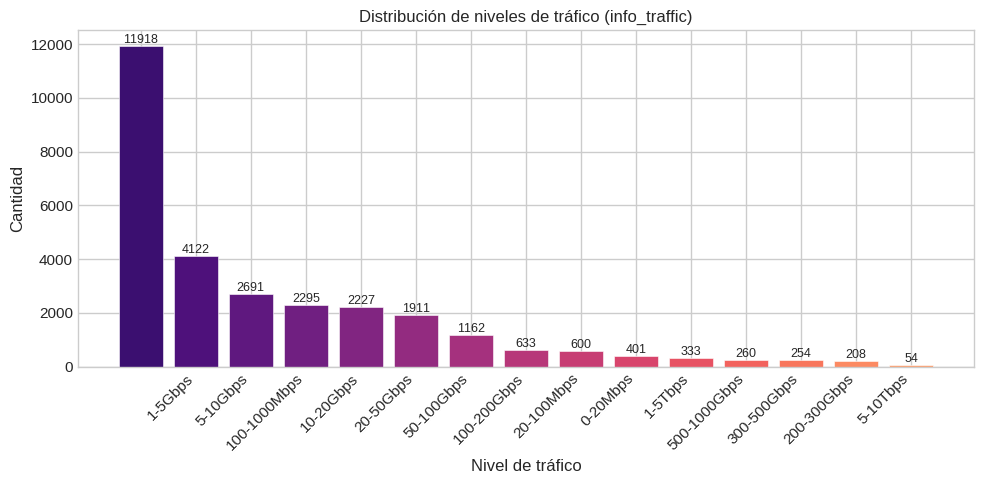
\includegraphics[width=\textwidth]{img/anexoPeeringDB/Distribución_de_niveles_de_tráfico_info_traffic.png}
%         \caption{Distribución de niveles de tráfico (\texttt{info\_traffic}).}
%         \label{fig:Distribución_de_niveles_de_tráfico_info_traffic}
%     \end{subfigure}
%     \hfill
%     \begin{subfigure}[b]{0.48\textwidth}
%         \centering
%         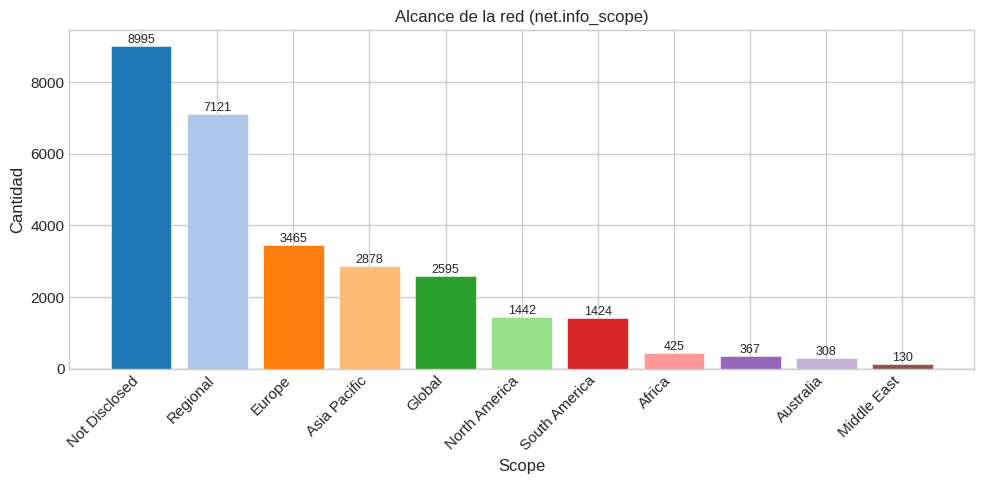
\includegraphics[width=\textwidth]{img/anexoPeeringDB/Alcance_de_la_red_info_scope.png}
%         \caption{Alcance de la red (\texttt{info\_scope}).}
%         \label{fig:Alcance_de_la_red_info_scope}
%     \end{subfigure}

%     % === 3ra fila ===
%     \vspace{5mm}
%     \begin{subfigure}[b]{0.48\textwidth}
%         \centering
%         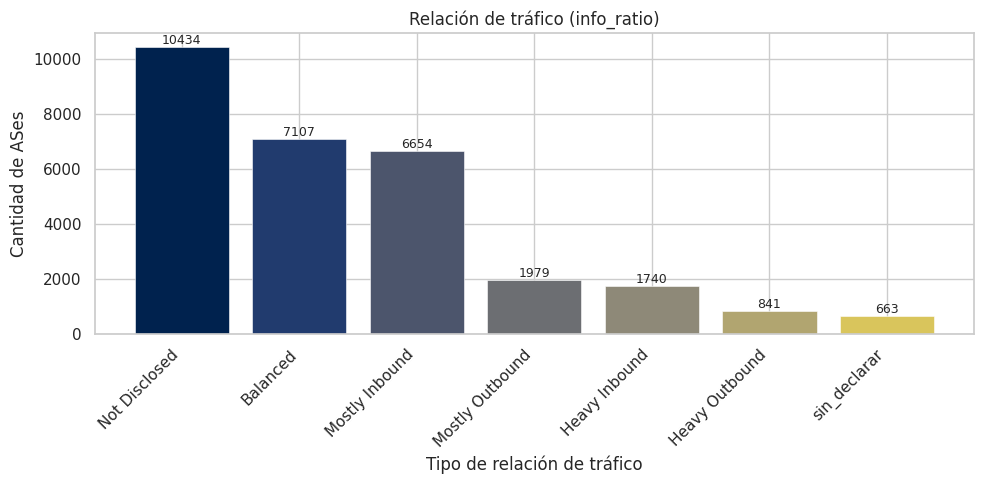
\includegraphics[width=\textwidth]{img/anexoPeeringDB/Relación_de_traficoinfo_ratio.png}
%         \caption{Relación de tráfico (\texttt{info\_ratio}).}
%         \label{fig:Relación_de_traficoinfo_ratio}
%     \end{subfigure}
%     \hfill
%     \begin{subfigure}[b]{0.48\textwidth}
%         \centering
%         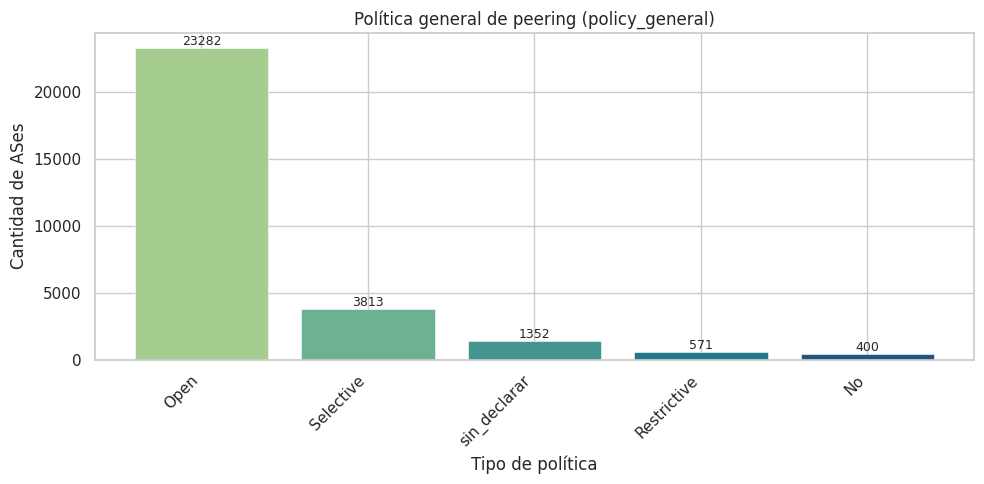
\includegraphics[width=\textwidth]{img/anexoPeeringDB/Politica_general_de_peering_policy_general.png}
%         \caption{Política general de peering (\texttt{policy\_general}).}
%         \label{fig:Politica_general_de_peering_policy_general}
%     \end{subfigure}

%     % === 4ta fila ===
%     \vspace{5mm}
%     \begin{subfigure}[b]{0.48\textwidth}
%         \centering
%         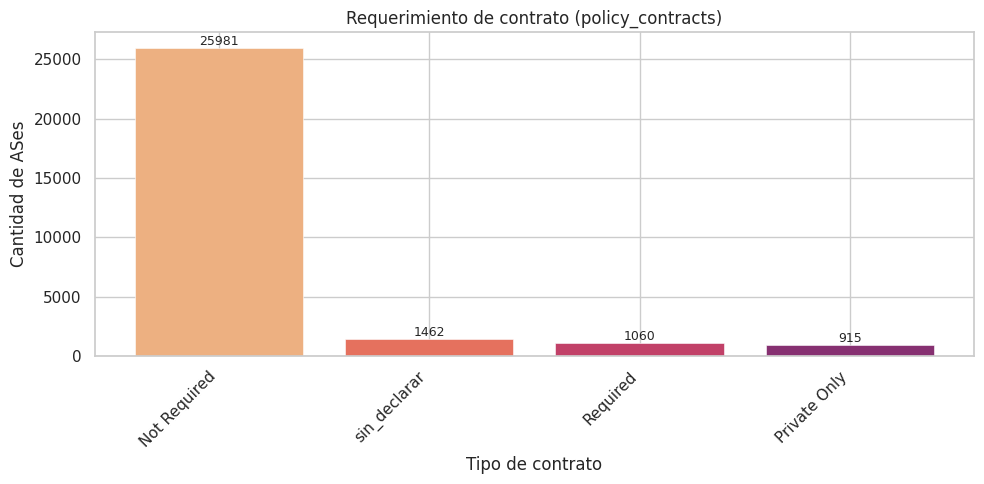
\includegraphics[width=\textwidth]{img/anexoPeeringDB/Requerimiento_de_contrato_policy_contracts.png}
%         \caption{Requerimiento de contrato (\texttt{policy\_contracts}).}
%         \label{fig:Requerimiento_de_contrato_policy_contracts}
%     \end{subfigure}
%     \hfill
%     \begin{subfigure}[b]{0.48\textwidth}
%         \centering
%         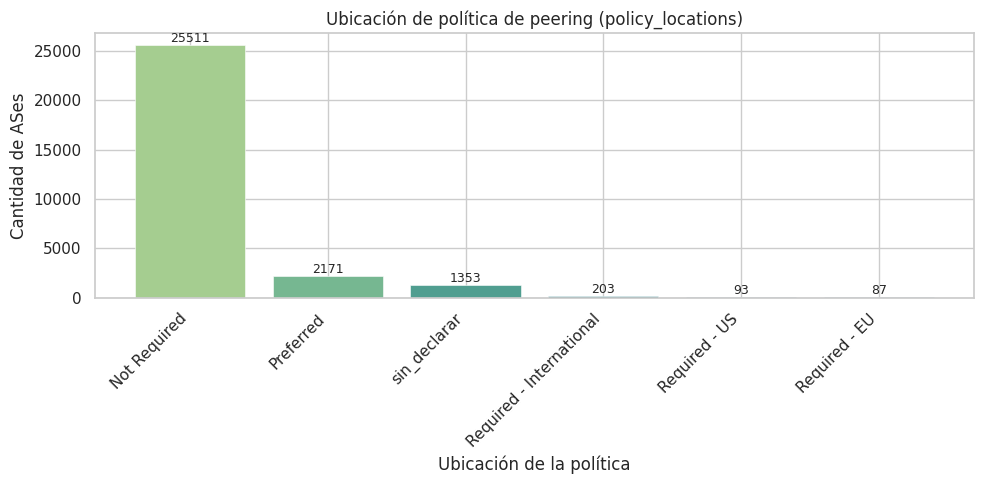
\includegraphics[width=\textwidth]{img/anexoPeeringDB/Ubicacion_de_política_de_peering_policy_locations.png}
%         \caption{Ubicación de política de peering (\texttt{policy\_locations}).}
%         \label{fig:Ubicacion_de_política_de_peering_policy_locations}
%     \end{subfigure}


%     \caption{Visualización general de las principales variables categóricas y numéricas del conjunto \texttt{net} de PeeringDB.}
%     \label{fig:graficos_peeringdb_completo}
% \end{figure}







% \begin{figure}[H]
%     \centering
%     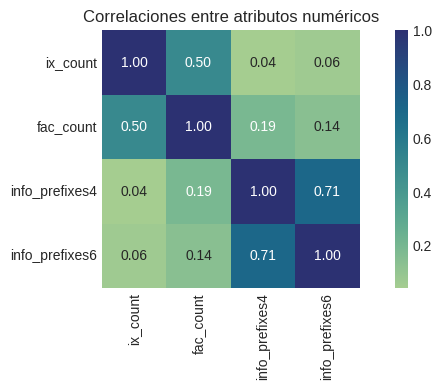
\includegraphics[width=0.6\textwidth]{img/anexoPeeringDB/Correlaciones_entre_atributos_numericos.png}
%     \caption{Matriz de correlación entre los atributos numéricos extraidos de PeeringDB.}
%     \label{fig:Correlaciones_entre_atributos_numericos}
% \end{figure}

% Con la visualización de la Figura~\ref{fig:Correlaciones_entre_atributos_numericos} podemos decir:
% \begin{itemize}
%     \item los AS que anuncian muchos prefijos IPv4 tienden también a anunciar muchos prefijos IPv6. Puedes esperar colinealidad entre ambos.
%     \item más IXPs suele venir acompañado de presencia en más facilities (tamaño/cobertura del AS).
% \end{itemize}



% \begin{table}[H]
% \centering
% \caption{Porcentaje de filas sin información por columna (antes de limpieza).}
% \label{tab:faltantes_net}
% \begin{tabular}{l l r r}
% \toprule
% \textbf{columna} & \textbf{tipo} & \textbf{sin\_info} & \textbf{porcentaje \%} \\
% \midrule
% info\_traffic      & categórica & 12047 & 40.95 \\
% info\_type         & categórica & 8439  & 28.69 \\
% policy\_contracts  & categórica & 1462  & 4.97  \\
% policy\_general    & categórica & 1352  & 4.60  \\
% policy\_locations  & categórica & 1353  & 4.60  \\
% info\_ratio        & categórica & 663   & 2.25  \\
% info\_scope        & categórica & 370   & 1.26  \\
% info\_prefixes4    & numérica   & 0     & 0.00  \\
% fac\_count         & numérica   & 0     & 0.00  \\
% ix\_count          & numérica   & 0     & 0.00  \\
% info\_prefixes6    & numérica   & 0     & 0.00  \\
% \bottomrule
% \end{tabular}
% \end{table}



% \subsection*{Exploración de IXPs}
% A modo de contexto, también se incluyen visualizaciones relacionadas con IXPs.

% \begin{figure}[H]
%     \centering
%     % === 1ra fila: dos figuras lado a lado ===
%     \begin{subfigure}[b]{0.48\textwidth}
%         \centering
%         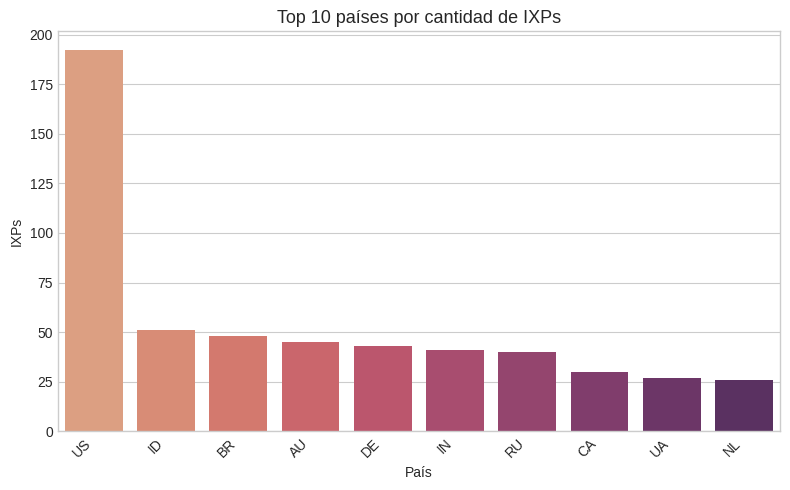
\includegraphics[width=\textwidth]{img/anexoPeeringDB/Top_10_países_por_cantidad_deI_XPs.png}
%         \caption{Top 10 países con mayor cantidad de IXPs registrados en PeeringDB.}
%         \label{fig:Top_10_países_por_cantidad_deI_XPs}
%     \end{subfigure}
%     \hfill
%     \begin{subfigure}[b]{0.48\textwidth}
%         \centering
%         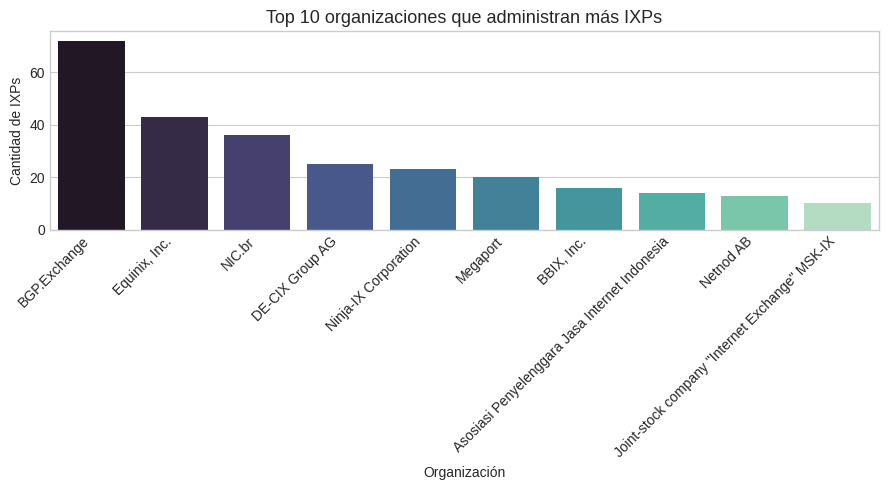
\includegraphics[width=\textwidth]{img/anexoPeeringDB/Top _10_organizaciones_que_administran_mas_IXPs.png}
%         \caption{Top organizaciones que administran mayor cantidad de IXPs registrados en PeeringDB.}
%         \label{fig:Top_10_org_por_cantidad_deI_XPs}
%     \end{subfigure}

%     % === 2da fila: figura centrada ===
%     \vspace{6mm}
%     \begin{subfigure}[b]{0.6\textwidth}
%         \centering
%         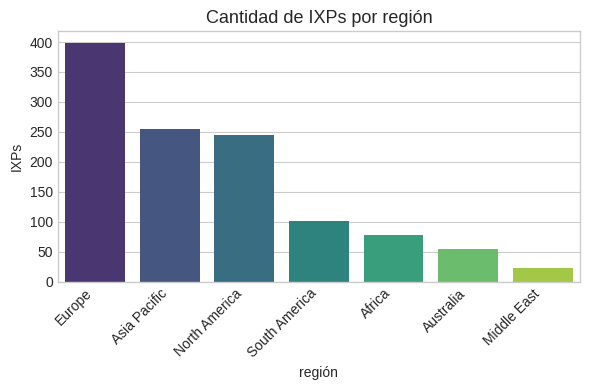
\includegraphics[width=\textwidth]{img/anexoPeeringDB/Cantida_de_IXPs_por_region.png}
%         \caption{Cantidad de IXPs por región.}
%         \label{fig:Cantida_de_IXPs_por_region}
%     \end{subfigure}

%     % === Caption general ===
%     \caption{Distribución y administración de IXPs registrados en PeeringDB: comparación por país, organización y región geográfica.}
%     \label{fig:ixps_peeringdb}
% \end{figure}



% \begin{table}
% \caption{IXPs registrados en Chile según PeeringDB (2024).}
% \label{tab:ixps_chile}
% \begin{tabular}{l l c}
% \toprule
% Nombre del IXP & Ciudad & País \\
% \midrule
% PIT Santiago - PIT Chile & Santiago & CL \\
% SCL-IX Chile & Santiago & CL \\
% PIT Concepcion - PIT Chile & Concepcion & CL \\
% PIT Osorno - PIT Chile & Osorno & CL \\
% PIT Temuco - PIT Chile & Temuco & CL \\
% PIT Arica - PIT Chile & Arica & CL \\
% PIT entel & Santiago & CL \\
% BGP.Exchange - Valdivia & Valdivia & CL \\
% BGP.Exchange - Santiago & Santiago & CL \\
% \bottomrule
% \end{tabular}
% \end{table}

% \section{Tabla Resumen Atributos de ASes de 
% trabajo~\cite{BenchmarkingGNN} }

% \begin{figure}[h!] % h! = aquí preferentemente
%     \centering
%     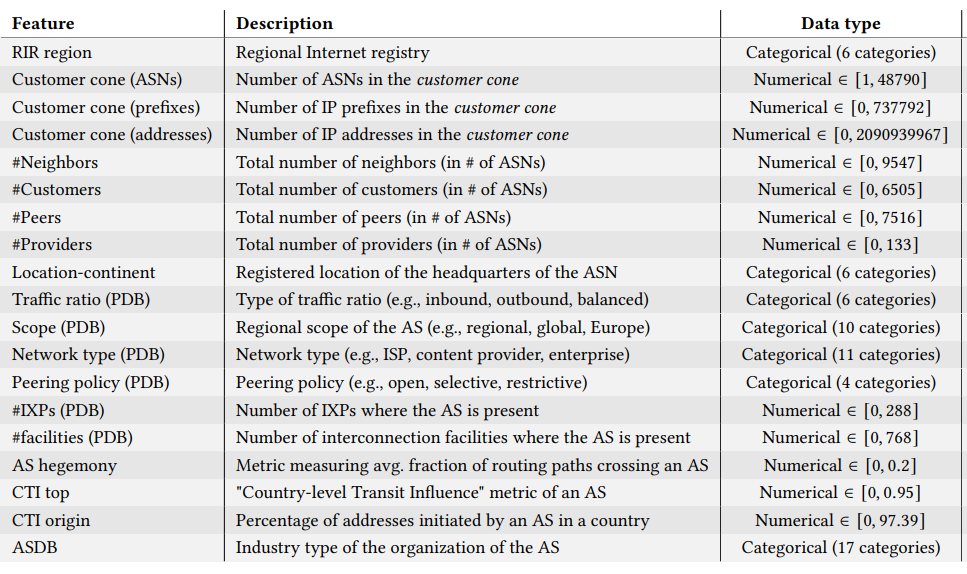
\includegraphics[width=0.9\textwidth]{img/metodologia/tabalAtributosgnnbchn.png}
%     \caption{Tabla resumen de atributos del paper ``\textit{Benchmarking Graph Neural Networks for Internet Routing Data}''.}
%     \label{tab:as_attr_tabla_bechmark}
% \end{figure}





% \section{Visualizaciones Grado de Salida de Datos de RIBs }


% Figura\ref{fig:cantidad_ases_rel_ribs} contiene Grafico cantidad de ASes y cantidad de relaciones por cada mes que se  extrajo las RIBs. Cada coleccion corresponde a las 12 primeras horas del primer dia del mes indicado.

% \begin{figure}[h]
%     \centering
%     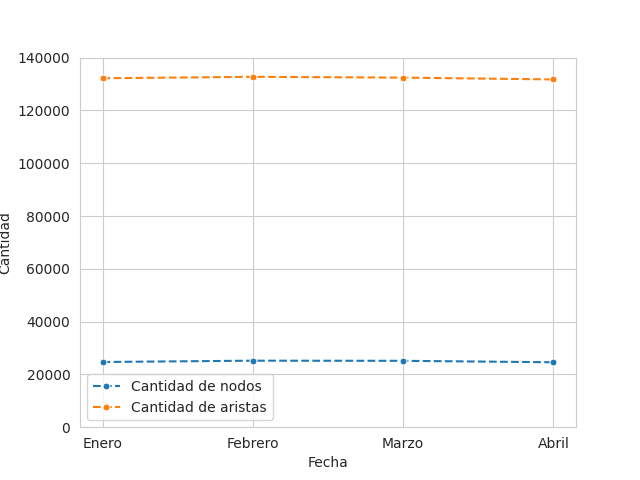
\includegraphics[width=0.7\textwidth]{img/resultados/cantidad_ases_rel_ribs.png}
%     \caption{Cantidad de relaciones y ASes para las diferentes fechas de los RIBs extraidos.}
%     \label{fig:cantidad_ases_rel_ribs}
% \end{figure}



% Figura~\ref{fig:top_20_as_febrero_numerorelaciones_src} complementaria que presenta el top 20 de ASes según su grado de salida. 

% \begin{figure}[H]
%     \centering
%     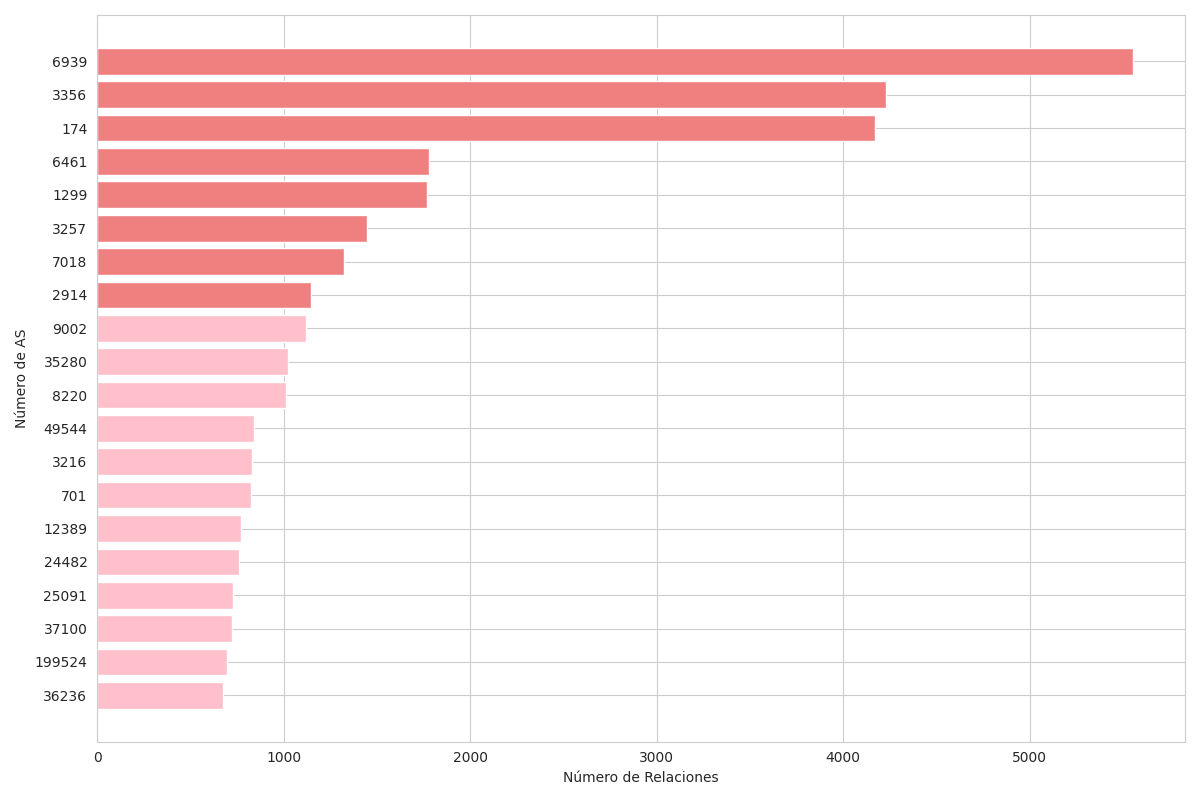
\includegraphics[width=0.9\textwidth]{img/resultados/top_20_as_febrero_numerorelaciones_src.png}
%     \caption{Top 20 ASes con mayor número de conexiones (grado), para RIB de febrero 2024.}
% \label{fig:top_20_as_febrero_numerorelaciones_src}
% \end{figure}


% La Figura~\ref{fig:distribucion_as_grado_salida_febrero_comparacion} muestra la distribución del grado de salida de los ASes en febrero, con y sin outliers. Este análisis se enfoca únicamente en las conexiones salientes, a diferencia del informe principal que considera el grado total (entradas y salidas).




% \begin{figure}[H]
%     \centering

%     \begin{subfigure}[b]{0.48\textwidth}
%         \centering
%         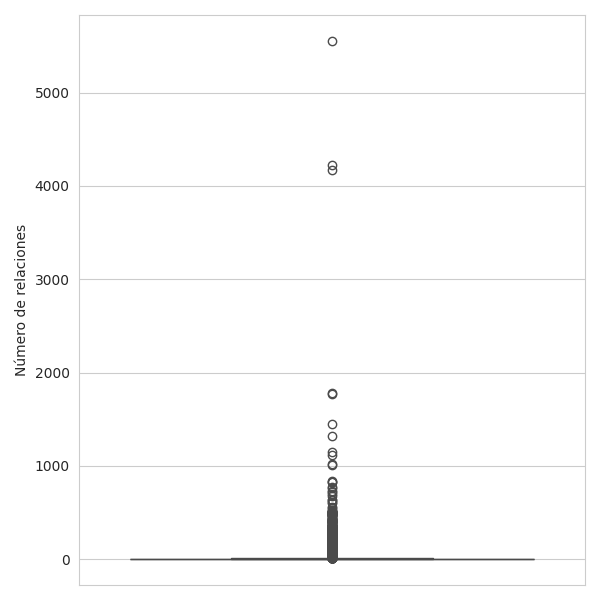
\includegraphics[width=\textwidth]{img/resultados/distribucion_as_grado_salida_febrero_boxplot_con_outliers.png}
%         \caption{Con outliers.}
%         \label{fig:distribucion_as_grado_salida_febrero_boxplot_con_outliers}
%     \end{subfigure}
%     \hfill
%     \begin{subfigure}[b]{0.48\textwidth}
%         \centering
%         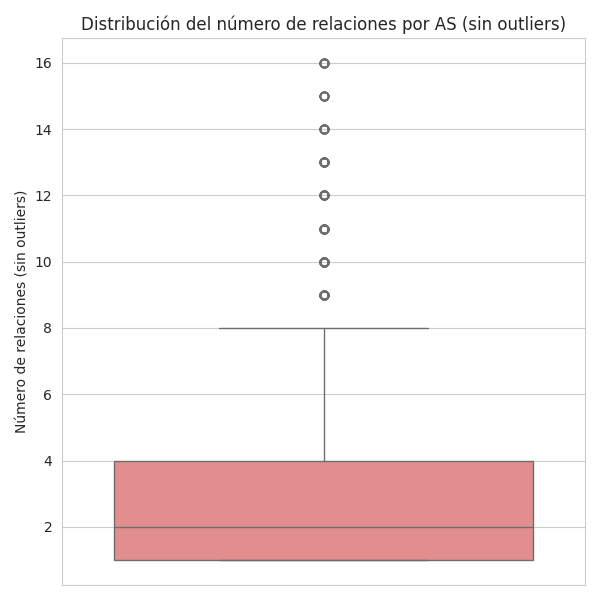
\includegraphics[width=\textwidth]{img/resultados/distribucion_as_grado_salida_febrero_boxplot_sin_outliers.png}
%         \caption{Sin outliers.}
%         \label{fig:distribucion_as_grado_salida_febrero_boxplot_sin_outliers}
%     \end{subfigure}


%     \caption{Comparación de la distribución del grado de salida de ASes en febrero, con y sin outliers.}
%     \label{fig:distribucion_as_grado_salida_febrero_comparacion}
% \end{figure}




% La Figura~\ref{fig:comparacion_mensual_largo_paths} muestra la distribución de la longitud de las rutas BGP observadas durante los primeros cuatro meses del año 2024.


% \section{Comparación mensual de la longitud de rutas}
% \begin{figure}[H]
%     \centering
%     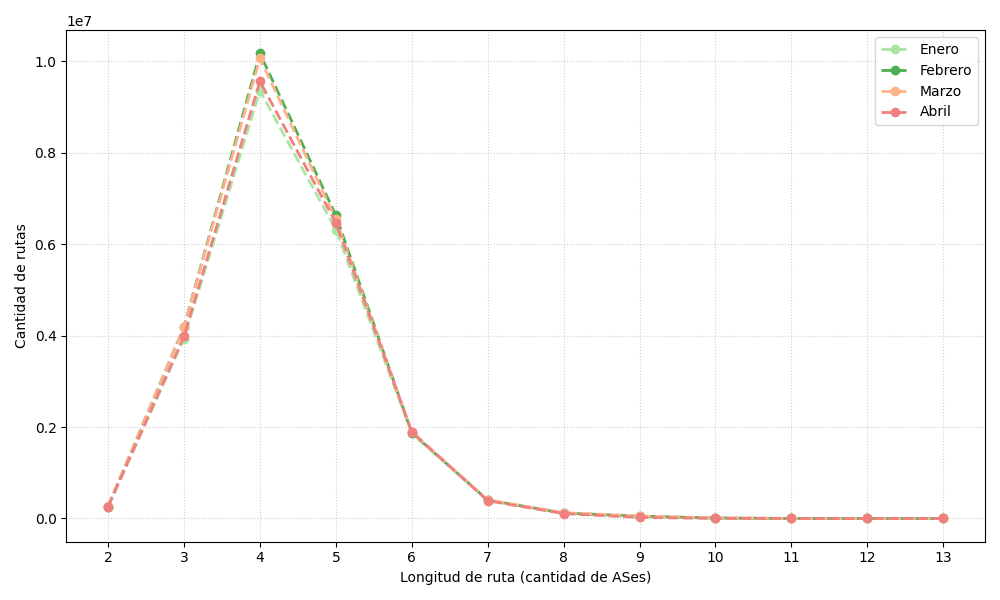
\includegraphics[width=0.8\textwidth]{img/resultados/comparacion_mensual_largo_paths.png}
%     \caption{Comparación mensual de la longitud de rutas BGP.}
% \label{fig:comparacion_mensual_largo_paths}
% \end{figure}










% \newpage
% \section{Cantidad de ASes y enlaces en dataset evaluacion} \label{sec:attr_asrank_section}


% \begin{table}[H]
% \centering
% \caption{Cantidad de ASes y aristas entre nodos en dataset de evaluacion asrank para los primeros 4 meses del ano}
% \begin{tabular}{lcc}
% \toprule
% \textbf{Mes} & \textbf{Numero de ASes } & \textbf{Enlaces totales} \\
% \midrule
% Enero   &  76.351 & 499.651 \\
% Febrero &  76.415 & 488.777 \\
% Marzo   &  76.551 & 492.945 \\
% Abril   &  76.644 & 495.601 \\
% \end{tabular}
% \label{tab:asrank_datasets}
% \end{table}


%\section{Palabras claras}
%\begin{itemize}
%    \item \textbf{Protocolos:} 
%    \item IRR: Internet Routing Registry. Base de datos que contiene información sobre los prefijos IP y los sistemas autónomos que los anuncian. Los IRRs son utilizados por los operadores de red para filtrar rutas BGP y prevenir el anuncio de rutas falsas.
%    \item RIR: Regional Internet Registry. Son organizaciones responsables de la asignacion y administracion de direcciones IP y numeros de Sistemas Autonomos (ASNs) en determinadas regiones geograficas.
%    \begin{itemize}
%        \item ARIN (American Registry for Internet Numbers): Norteamerica, el Caribe y Africa Subsahariana.
%        \item RIPE NCC (Réseaux IP Européens Network Coordination Centre): Europa, Oriente Medio y Asia Central.
%        \item APNIC (Asia-Pacific Network Information Centre): Asia y el Pacifico.
%        \item  LACNIC (Latin American and Caribbean Network Information Centre): America Latina y el Caribe.
%        \item AfriNIC (African Network Information Centre): Africa.
%    \end{itemize} 
%    \item AS: Sistema Autono y Autonomous System en ingles.
%    \item BGP: Border Gateway Protocol
%    \item RRC: Route Collectors
%    \item IXP: Internet Exchange Point
%    \item Internet Carrier*: Empresas que operan infrestructras de Red de gran escala. Ofrecen servicios de intercambio de datos.
%    Forman parte del nucleo de Internet.
%    ejemplos de carrier son: AT\&T.
%    \item ISP: Internet Service Provider
%    \item CDN: Content Delivery Network
%    \item ASN: Número de sistema autónomo, un número entero de 32 bits que identifica de forma única una red. Por ejemplo, uno de los ASN de Cloudflare (tenemos varios) es 13335.
    
%    \item content provider network: Red privada que conecta sus centros de datos a Internet, a menudo evitando los ISP regionales de nivel 1.\cite{Computer-Networking}

%\item Internet Service Provider (ISP): Proveedor de servicios de Internet. Empresa que ofrece servicios de acceso a Internet a usuarios finales. Se encuentras en la parte mśa oeriferica de la red de Internt


%\item Prefijos IP: un prefijo IP es un rango de direcciones IP, agrupadas en potencias de dos. En el espacio IPv4, dos direcciones forman un prefijo /31, cuatro forman un /30, y así sucesivamente, hasta /0, que es la abreviatura de "todos los prefijos de IPv4". Lo mismo aplica para IPv6, pero en lugar de agregar 32 bits como máximo, puede agregar hasta 128 bits. La siguiente figura muestra esta relación entre los prefijos IP, a la inversa: un /24 contiene dos /25 que contienen dos /26 y así sucesivamente

%\item Clique: Un conjunto de Sistemas Autonomos que estan interconectados, es decir,cada AS dentro del clique tiene una conexion directa con todos los demas AS dentro del clique. Este tipo de estructura suele encontrarse  en la capa más alta de la jerarquía   de tinterent, conocida como Tier-1 ASes.

%\item IANA:


%\end{itemize}




% \section{Attributos de los Sistemas Autonomos} \label{sec:attr_as_section}

% \begin{table}[ht]
% \centering
% \footnotesize
% \begin{tabular}{|p{5cm}|p{4.5cm}|}
% \hline
% \textbf{Atributo categórico} & \textbf{Clases posibles} \\
% \hline

% \multirow{4}{*}{policy\_general} 
% & Restrictive \\
% & Open \\
% & Selective \\
% & None \\
% \hline

% \multirow{6}{*}{policy\_locations} 
% & Required - International \\
% & Not Required \\
% & Preferred \\
% & Required - US \\
% & Required - EU \\
% & None \\
% \hline

% \multirow{4}{*}{policy\_contracts} 
% & Required \\
% & Not Required \\
% & Private Only \\
% & None \\
% \hline

% \multirow{10}{*}{info\_scope} 
% & Global \\
% & Europe \\
% & North America \\
% & Regional \\
% & Asia Pacific \\
% & South America \\
% & Not Disclosed \\
% & Australia \\
% & Middle East \\
% & None \\
% \hline

% \multirow{5}{*}{info\_ratio} 
% & Heavy Outbound \\
% & Heavy Inbound \\
% & Mostly Outbound \\
% & Mostly Inbound \\
% & Balanced \\
% \hline

% \multirow{12}{*}{info\_type} 
% & NSP \\
% & Content \\
% & Non-Profit \\
% & Cable/DSL/ISP \\
% & Enterprise \\
% & Educational/Research \\
% & Route Server \\
% & Route Collector \\
% & Not Disclosed \\
% & Network Services \\
% & Government \\
% & None \\
% \hline
% \end{tabular}
% \caption{Atributos categóricos y sus clases posibles utilizadas en la clasificación de nodos.}
% \label{tab:categorical_classes_node_classification}
% \end{table}




%\newpage
%\section{Benchmarck} 
%\label{sec:bechmark_resultados}





%\begin{table}[ht]
%\centering
%\begin{tabular}{lccccc}
%\hline
%\textbf{Método} & \textbf{presicion p2p} & \textbf{presicion c2p} & %\textbf{presicion p2c}\\
%\hline
%Gao & 0.96 & 0.78 & 0.78  \\
%Ruan & 0.93 & 0.63 & 0.63 \\
%ProbLink & 0.00 & 0.00 & 0.00 \\
%TopoScope & 0.92 & 0.98 & 0.99\\
%bgp2vec & 0.97 & 0.88 & 0.89\\
%\hline
%\end{tabular}
%\caption{Comparación de resultados de %\textit{accuracy} entre distintos metodos con 1 millon de rutas como entrada}
%\label{tab:comparacion_presicion}
%\end{table}

%\begin{table}[ht]
%\centering
%\begin{tabular}{lccccc}
%\hline
%\textbf{Método} & \textbf{recall p2p} %& \textbf{recall c2p} & \textbf{recall p2c}\\
%\hline
%Gao & 0.56 & 0.98 & 0.98  \\
%Ruan & 0.10 & 0.99 & 0.99 \\
%ProbLink & 0.00 & 0.00 & 0.00 \\
%TopoScope & 0.99 & 0.83 & 0.83\\
%bgp2vec &0.96 & 0.90 & 0.89\\
%\hline
%\end{tabular}
%\caption{Comparación de resultados de %\textit{accuracy} entre distintos metodos con 1 millon de rutas como entrada}
%\label{tab:comparacion_recall}
%\end{table}

%\begin{table}[ht]
%\centering
%\begin{tabular}{lccccc}
%\hline
%\textbf{Método} & \textbf{f1-score p2p} & \textbf{f1-score c2p} & %\textbf{f1-score p2c}\\
%\hline
%Gao & 0.71 & 0.87 & 0.87  \\
%Ruan & 0.19 & 0.77 & 0.77 \\
%ProbLink & 0.00 & 0.00 & 0.00 \\
%TopoScope & 0.96 & 0.90 & 0.90\\
%bgp2vec &0.97 & 0.89 & 0.89\\
%\hline
%\end{tabular}
%\caption{Comparación de resultados de %\textit{accuracy} entre distintos metodos con 1 millon de rutas como entrada}
%\label{tab:comparacion_f1_score}
%\end{table}






%\subsection{Estudio Atributos Dataset PeeringDB} \label{sec:estudio_attr_peeringdb_anexo}


%\section{Arquitecturas de Redes Neuronales de Grafo (GNNs)}

%\subsection{Enfoque por partes}



%\subsubsection{Caso 1: Atributos basados en grado con predicción de enlaces}\label{sec:anexo_por_partes_caso_1}


%\subsubsubsection{Análisis de Enlaces con Limitación de 1.000.000 AS\_PATHS} \label{sec:caso11_limitacion_1millon_resultados_Anexo}


%Resultados obtenidos al generar los embeddings a partir de 1.000.000 de rutas AS\_PATH. Tabla \ref{tab:accuracy_gnn_case11} presenta los valores de AUC y accuracy obtenidos por cada combinación de encoder y decoder. La Figura \ref{fig:comparacion_roc_auc_caso1_anexo} complementa esta información mostrando las curvas ROC y la distribución de los casos positivos y negativos.\\


%\begin{table}[H]
%\centering
%\begin{tabular}{lccc}
%\hline
%\textbf{Modelo} & \textbf{Decodificador} & \textbf{AUC} &\textbf{Accuracy (\%)} \\
%\hline
%GCN & Dot Product&  0.748 & 70.86\% \\
%GraphSAGE & Dot Product& 0.766 &  72.46\% \\
%GAT & Dot Product & 0.746 & 70.83\% \\  
%GCN & MLP& 0.958 & 71.41\% \\  
%GraphSAGE& MLP & 0.912 & 70.39\% \\
%GAT & MLP& 0.943 & 70.66\% \\  
%\hline
%\end{tabular}
%\caption{Resultados de AUC y Accuracy Inferencia para diferentes combinaciones de GNN y decoders.}
%\label{tab:accuracy_gnn_case11}
%\end{table}



%\begin{figure}[H]
%    \centering
    % Primera fila
%    \begin{subfigure}[b]{0.45\textwidth}
%        \centering
%        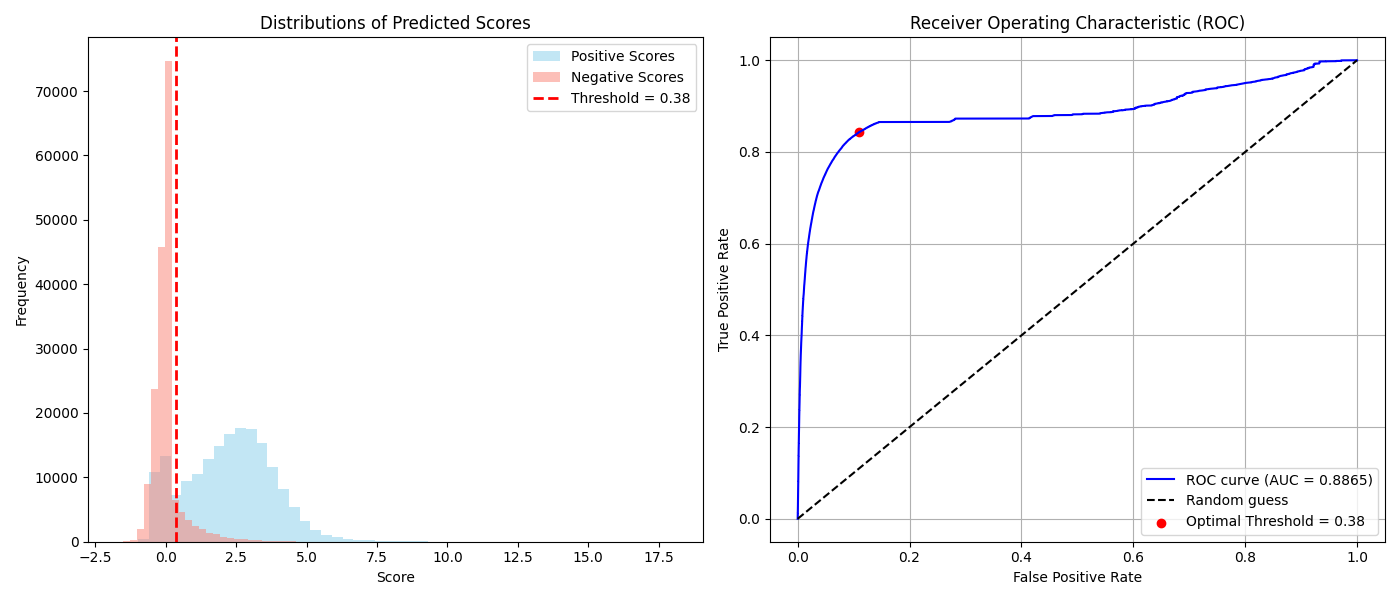
\includegraphics[width=\textwidth]{img/resultados/gnn/partes/caso1_degree/curva_roc/roc_curve_GCN_DotProduct_degree.png}
%        \caption{GCN + Dot Product}
%        \label{fig:conf_matrix_gcn_dp}
%    \end{subfigure}
%    \hfill
%    \begin{subfigure}[b]{0.45\textwidth}
%        \centering
%        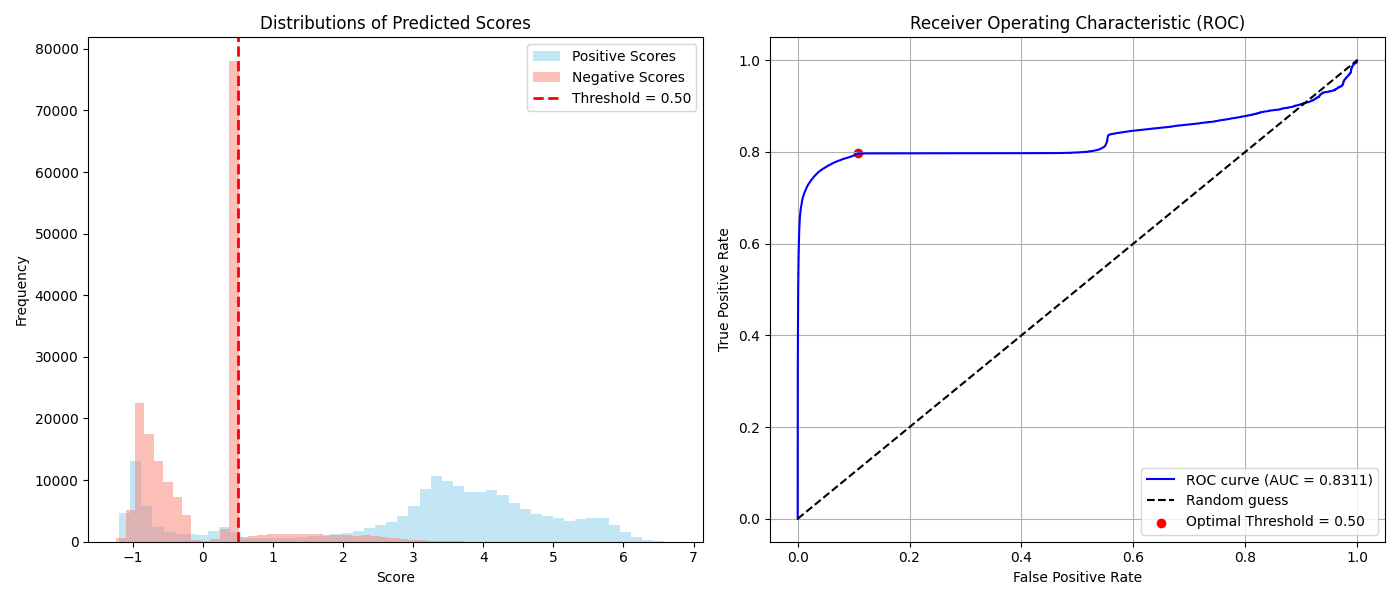
\includegraphics[width=\textwidth]{img/resultados/gnn/partes/caso1_degree/curva_roc/roc_curve_GraphSAGE_DotProduct_degree.png}
%        \caption{GraphSAGE + Dot Product}
%        \label{fig:conf_matrix_sage_dp}
%    \end{subfigure}
%    \vspace{0.5cm}

    % Segunda fila
%    \begin{subfigure}[b]{0.45\textwidth}
%        \centering
%        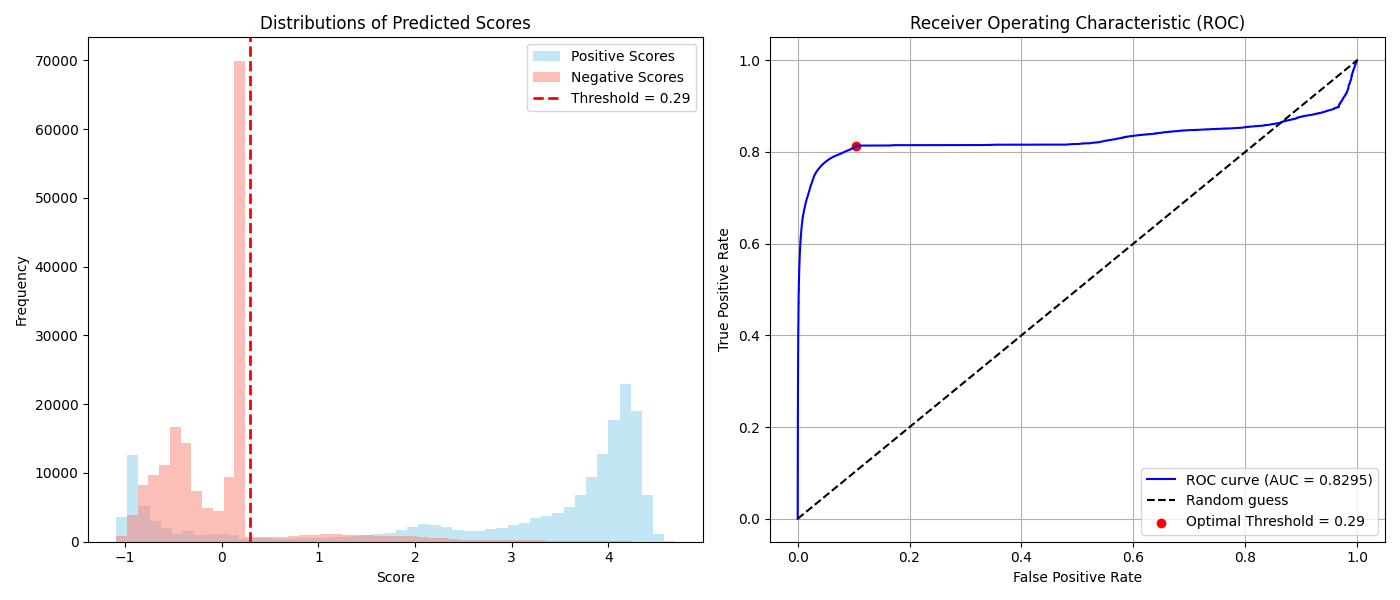
\includegraphics[width=\textwidth]{img/resultados/gnn/partes/caso1_degree/curva_roc/roc_curve_GAT_DotProduct_degree.png}
%        \caption{GAT + Dot Product}
%        \label{fig:conf_matrix_gat_dp}
%    \end{subfigure}
%    \hfill
%    \begin{subfigure}[b]{0.45\textwidth}
%        \centering
%        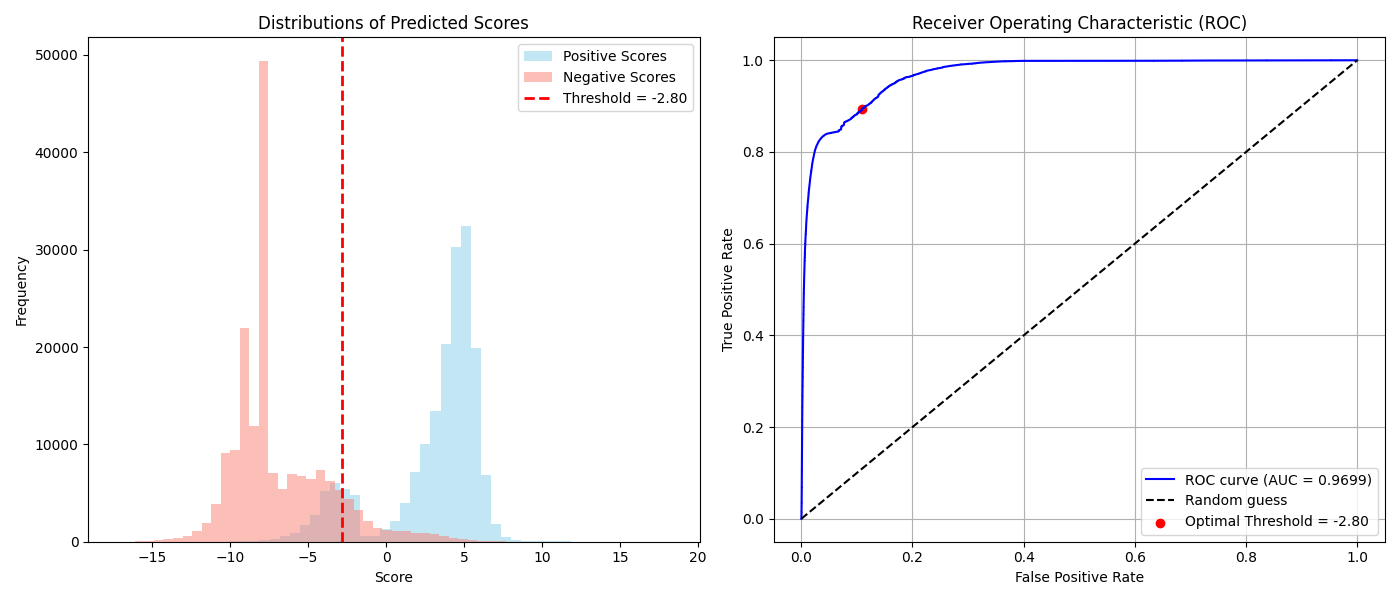
\includegraphics[width=\textwidth]{img/resultados/gnn/partes/caso1_degree/curva_roc/roc_curve_GCN_MLP_degree.png}
%        \caption{GCN + MLP}
%        \label{fig:conf_matrix_gcn_mlp}
%    \end{subfigure}

%    \vspace{0.5cm}

    % Tercera fila
%    \begin{subfigure}[b]{0.45\textwidth}
%        \centering
%        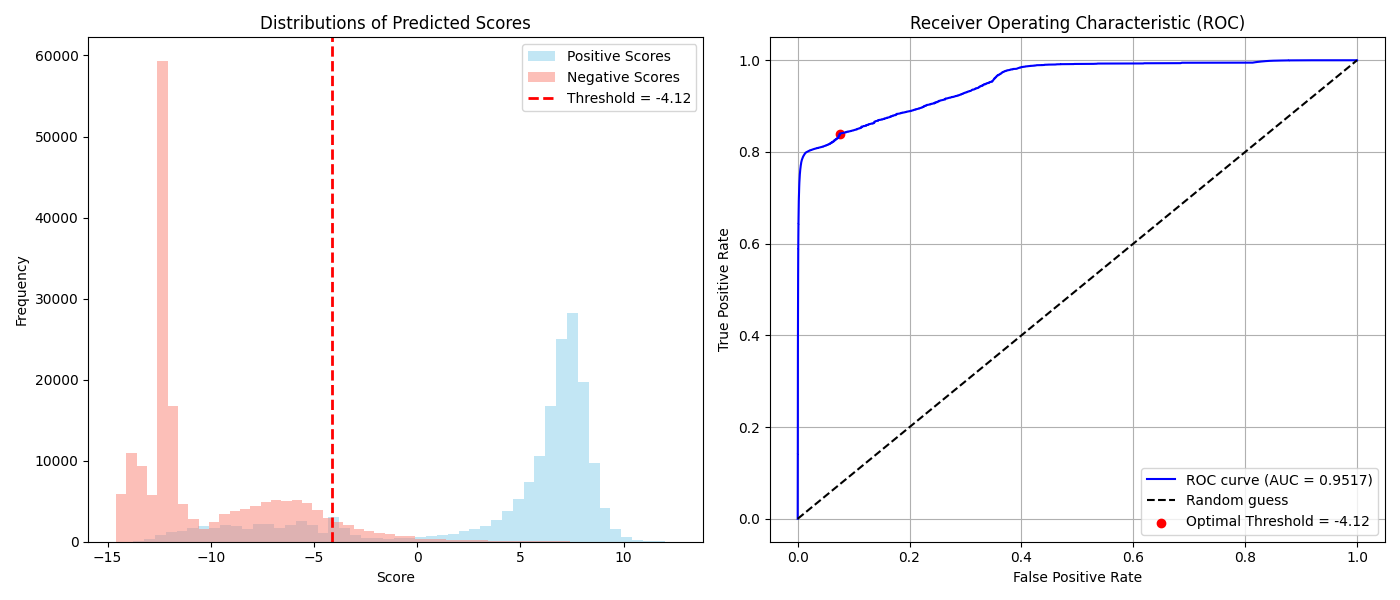
\includegraphics[width=\textwidth]{img/resultados/gnn/partes/caso1_degree/curva_roc/roc_curve_GraphSAGE_MLP_degree.png}
%        \caption{GraphSAGE + MLP}
%        \label{fig:conf_matrix_sage_mlp}
%    \end{subfigure}
%    \hfill
%    \begin{subfigure}[b]{0.45\textwidth}
%        \centering
%        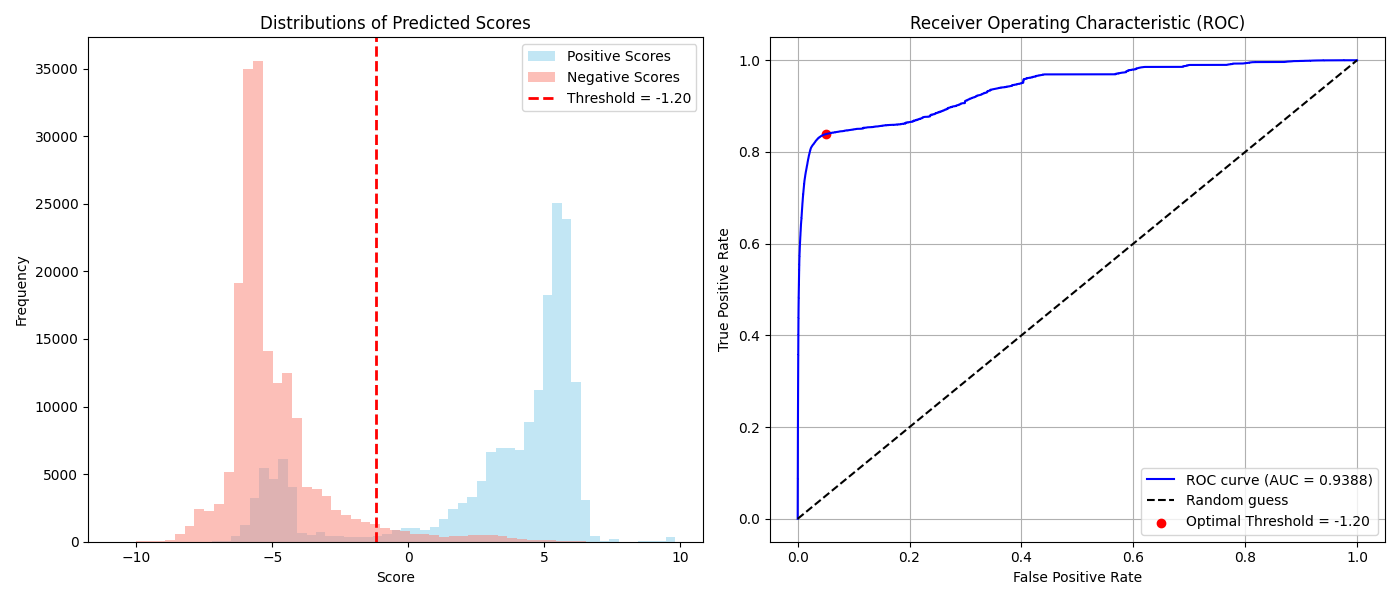
\includegraphics[width=\textwidth]{img/resultados/gnn/partes/caso1_degree/curva_roc/roc_curve_GAT_MLP_degree.png}
%        \caption{GAT + MLP}
%        \label{fig:conf_matrix_gat_mlp}
%    \end{subfigure}
%    \caption{Curvas ROC y distribución de resultados con el mejor umbral.}
%    \label{fig:comparacion_roc_auc_caso1_anexo}
%\end{figure}

%\subsubsubsection{Resultados Matriz de Confusión} \label{sec:mc_degree_full}
%\begin{figure}[H]
%    \centering
%    % Primera fila ////////////////////////////////////////////
%    \begin{subfigure}[b]{0.24\textwidth}
%        \centering
%        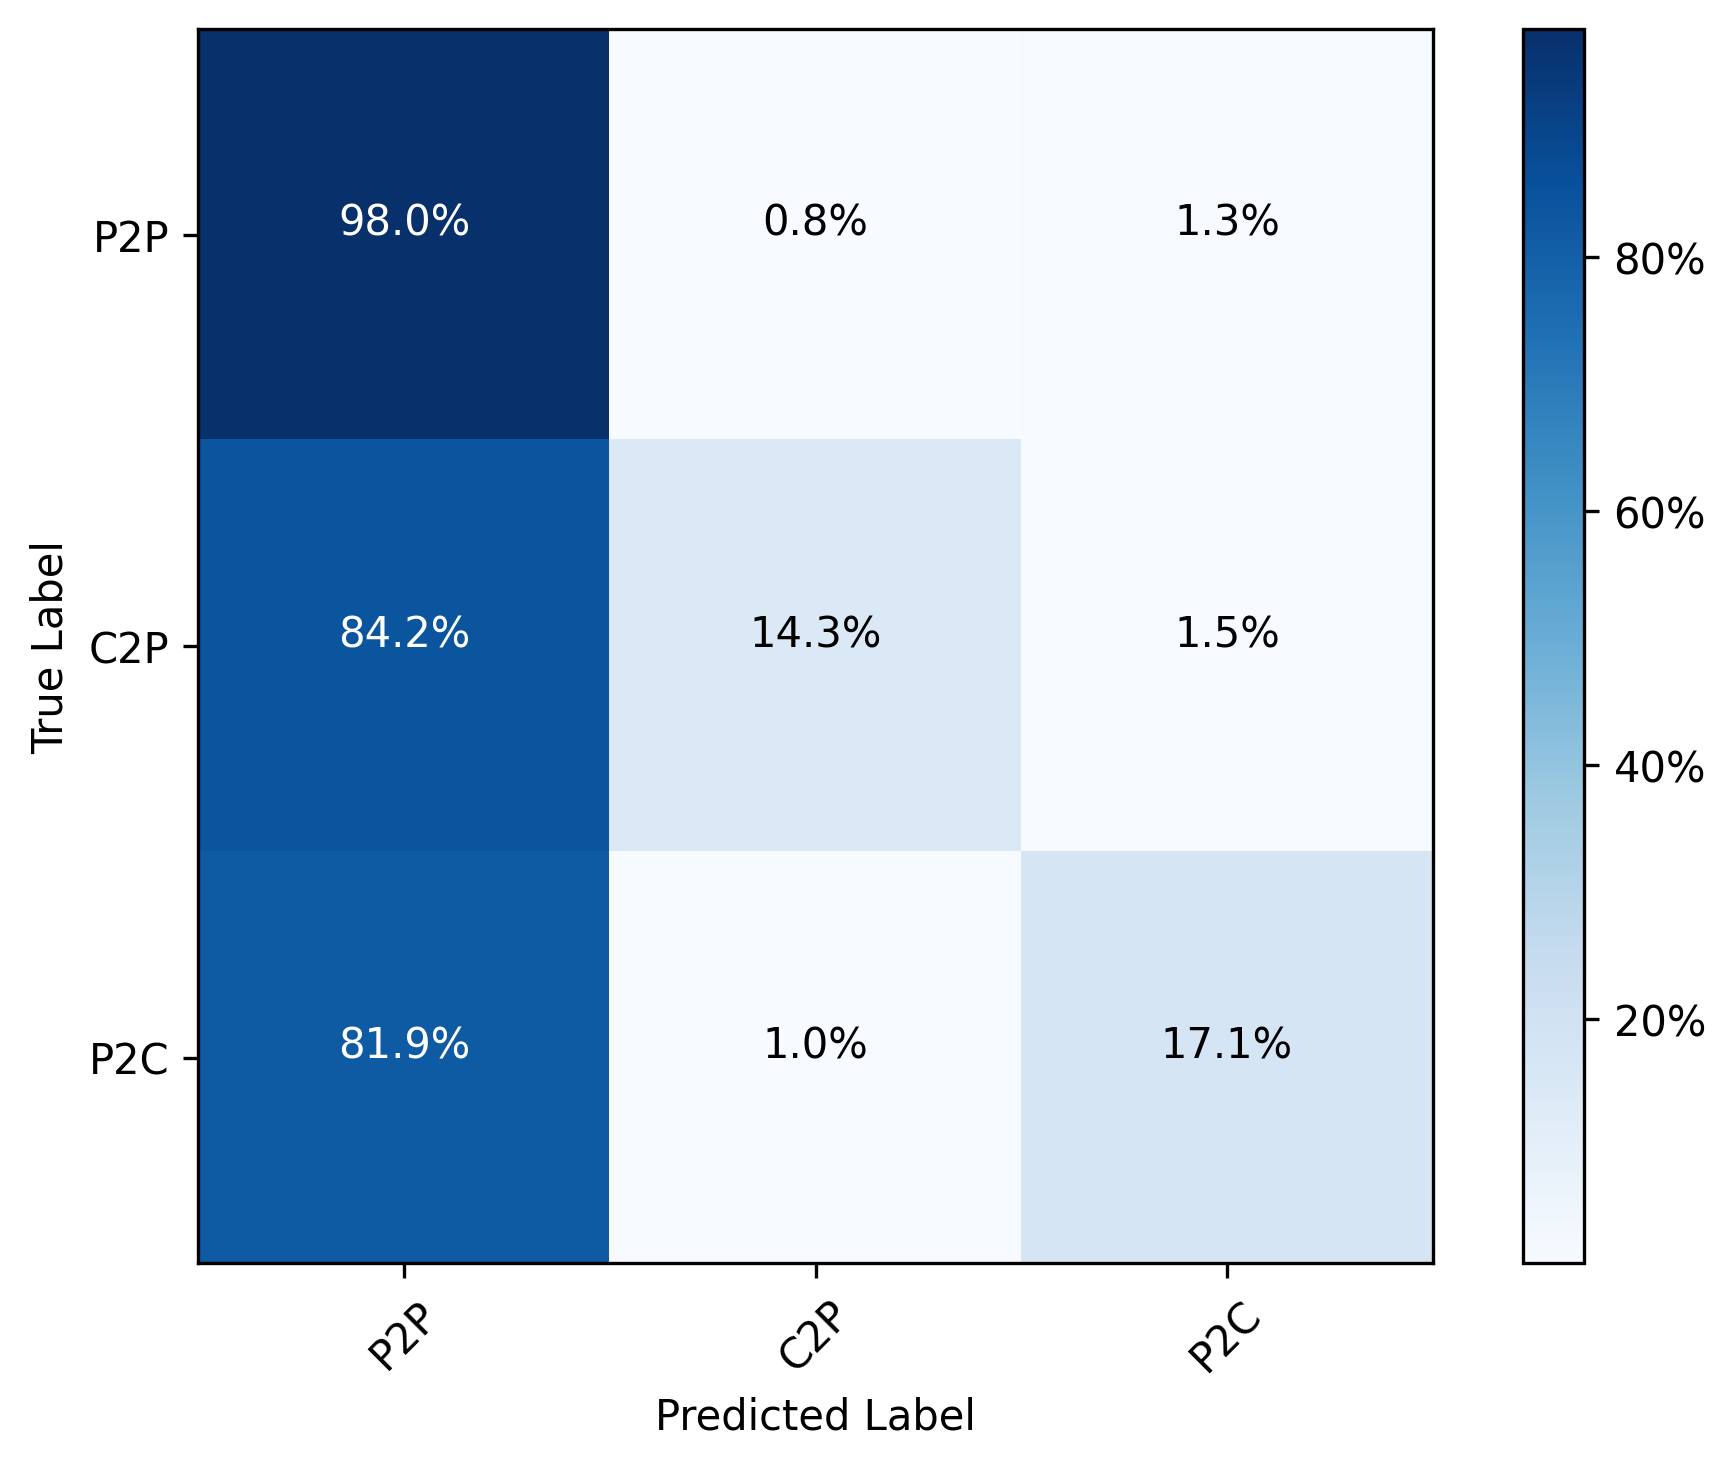
\includegraphics[width=\textwidth]{img/resultados/gnn/partes/caso1_degree/full/Confusion matrix_normalized_febrero_embeddings_ribs_DotProduct_GCN_grado_attr_febrero_with_no_batches_with_no_class_weight}
%        \caption{GCN·DP\\ 
%        NoBatch-NoW}
%        \label{fig:conf_matrix_gcn_dp}
%    \end{subfigure}
%    \hfill
%    \begin{subfigure}[b]{0.24\textwidth}
%        \centering
%        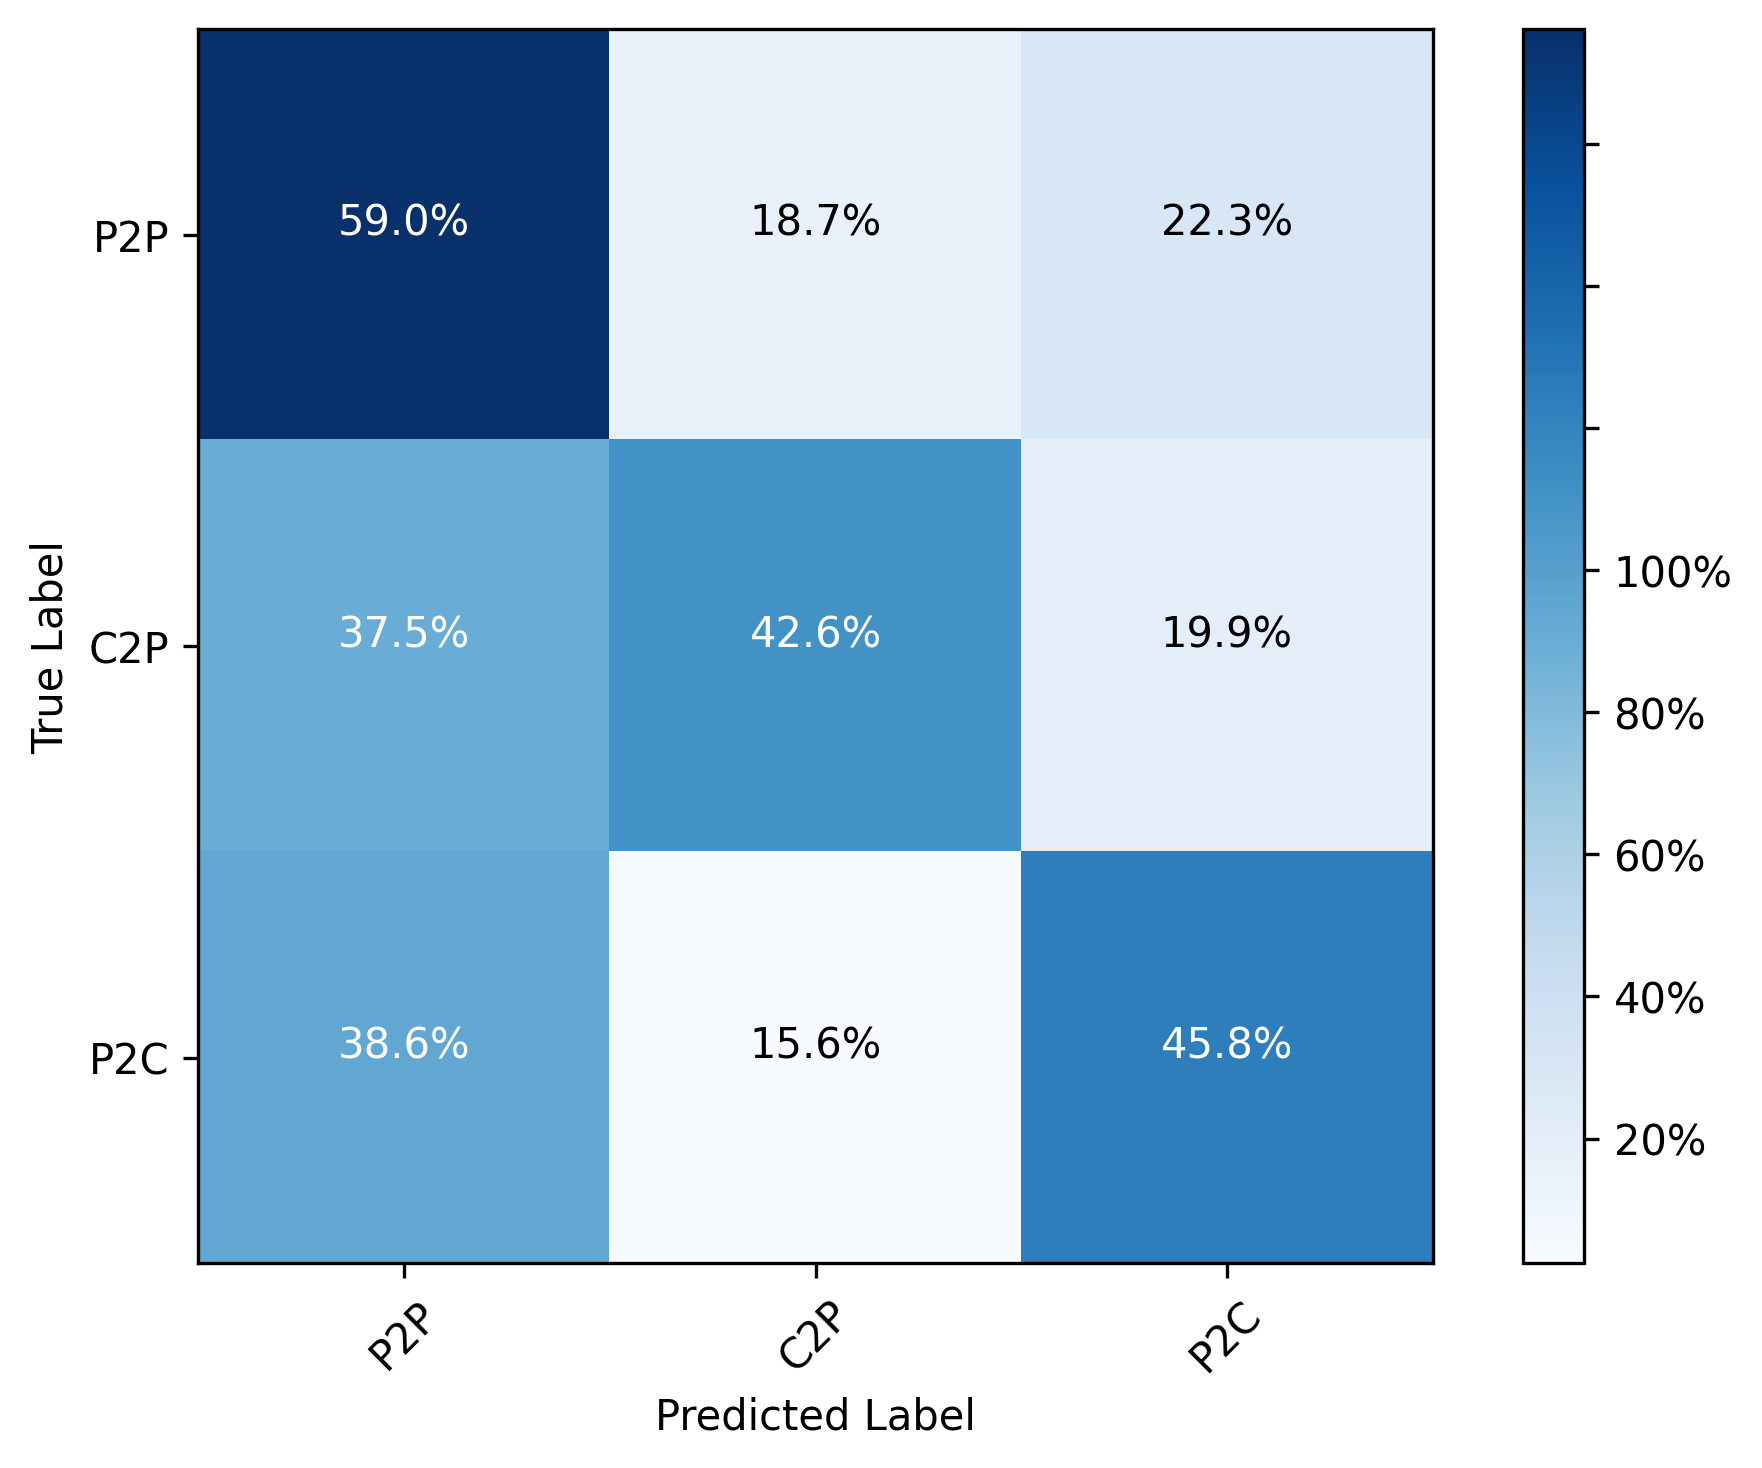
\includegraphics[width=\textwidth]{img/resultados/gnn/partes/caso1_degree/full/Confusion matrix_normalized_febrero_embeddings_ribs_DotProduct_GCN_grado_attr_febrero_with_no_batches_with_class_weight}
%        \caption{GCN·DP – NoBatch-W }
%        \label{fig:conf_matrix_sage_dp}
%    \end{subfigure}
%    \hfill
%    \begin{subfigure}[b]{0.24\textwidth}
%        \centering
%        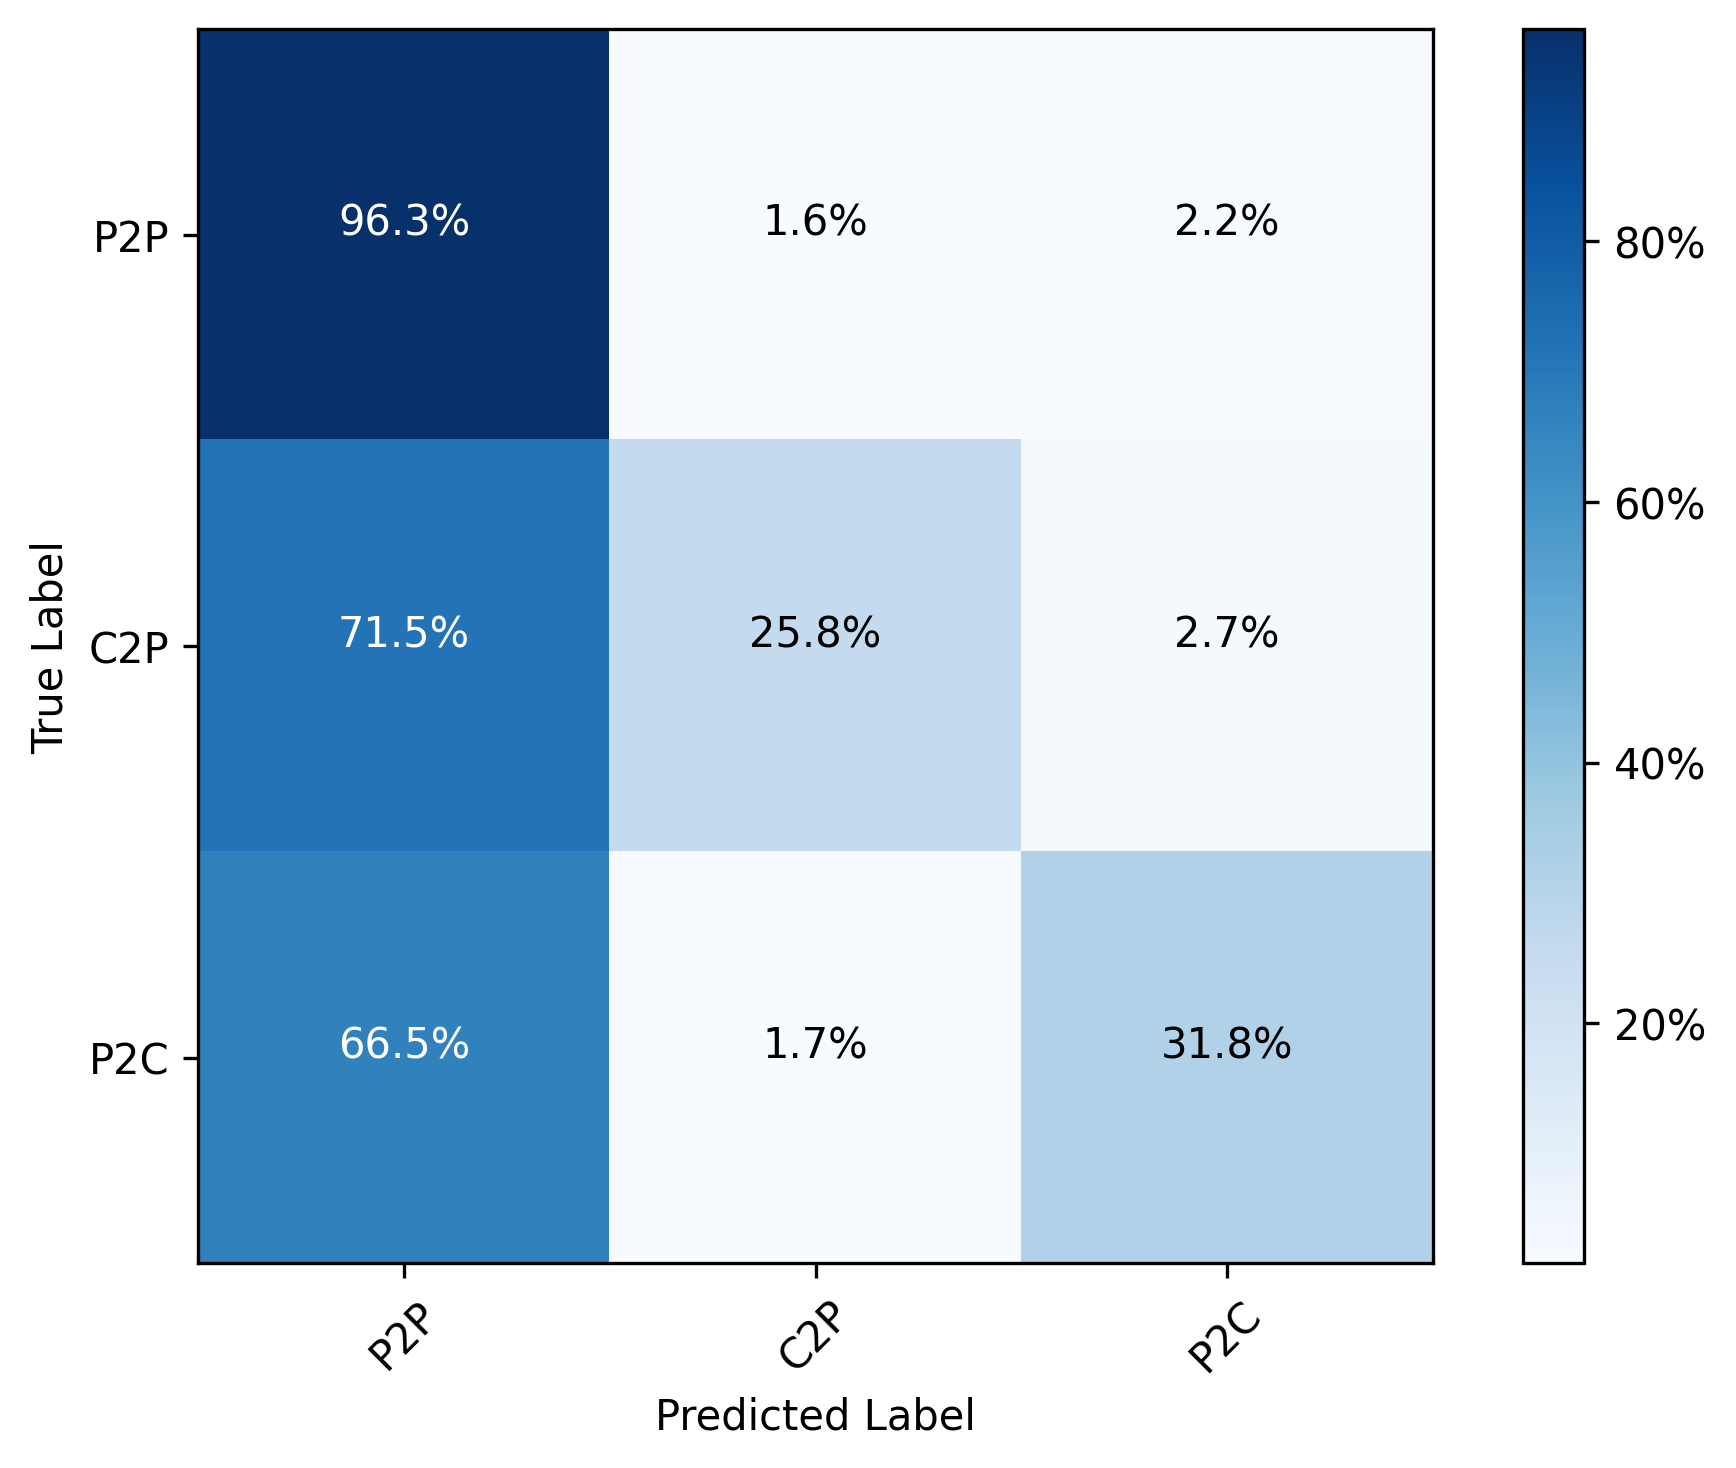
\includegraphics[width=\textwidth]{img/resultados/gnn/partes/caso1_degree/full/Confusion matrix_normalized_febrero_embeddings_ribs_DotProduct_GCN_grado_attr_febrero_with_batches_with_no_class_weight}
%        \caption{GCN·DP – Batch-NoW }
%        \label{fig:conf_matrix_gat_dp}
%    \end{subfigure}
%    \hfill
%    \begin{subfigure}[b]{0.24\textwidth}
%        \centering
%        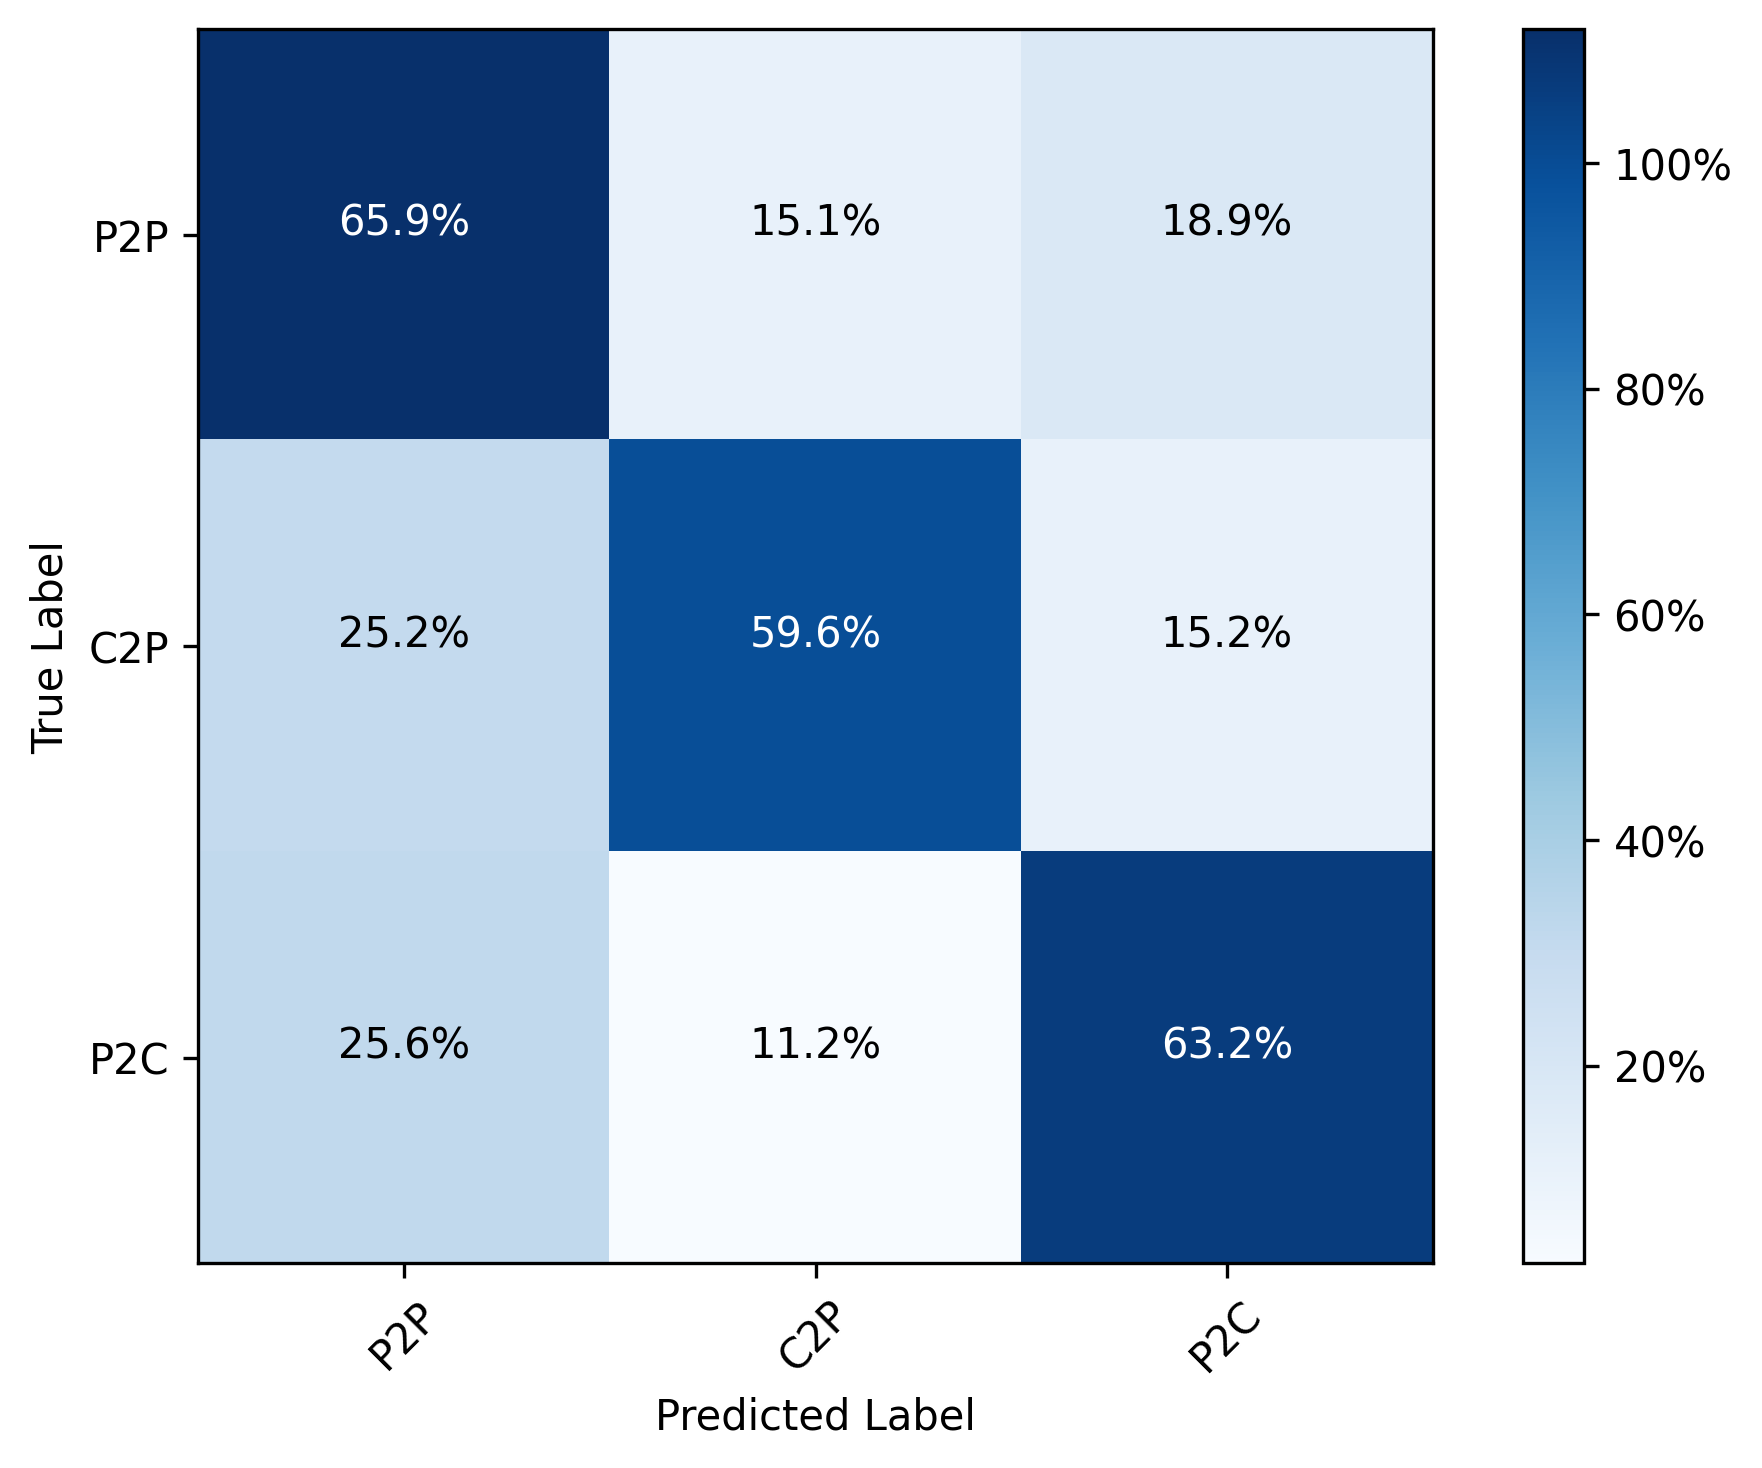
\includegraphics[width=\textwidth]{img/resultados/gnn/partes/caso1_degree/full/Confusion matrix_normalized_febrero_embeddings_ribs_DotProduct_GCN_grado_attr_febrero_with_batches_with_class_weight}
%        \caption{GCN·DP – Batch-W }
%        \label{fig:conf_matrix_gat_dp}
%    \end{subfigure}
%
%\end{figure}
%\begin{figure}[H]
%    \centering
%    % Segunda fila ////////////////////////////////////////
%    \begin{subfigure}[b]{0.24\textwidth}
%        \centering
%        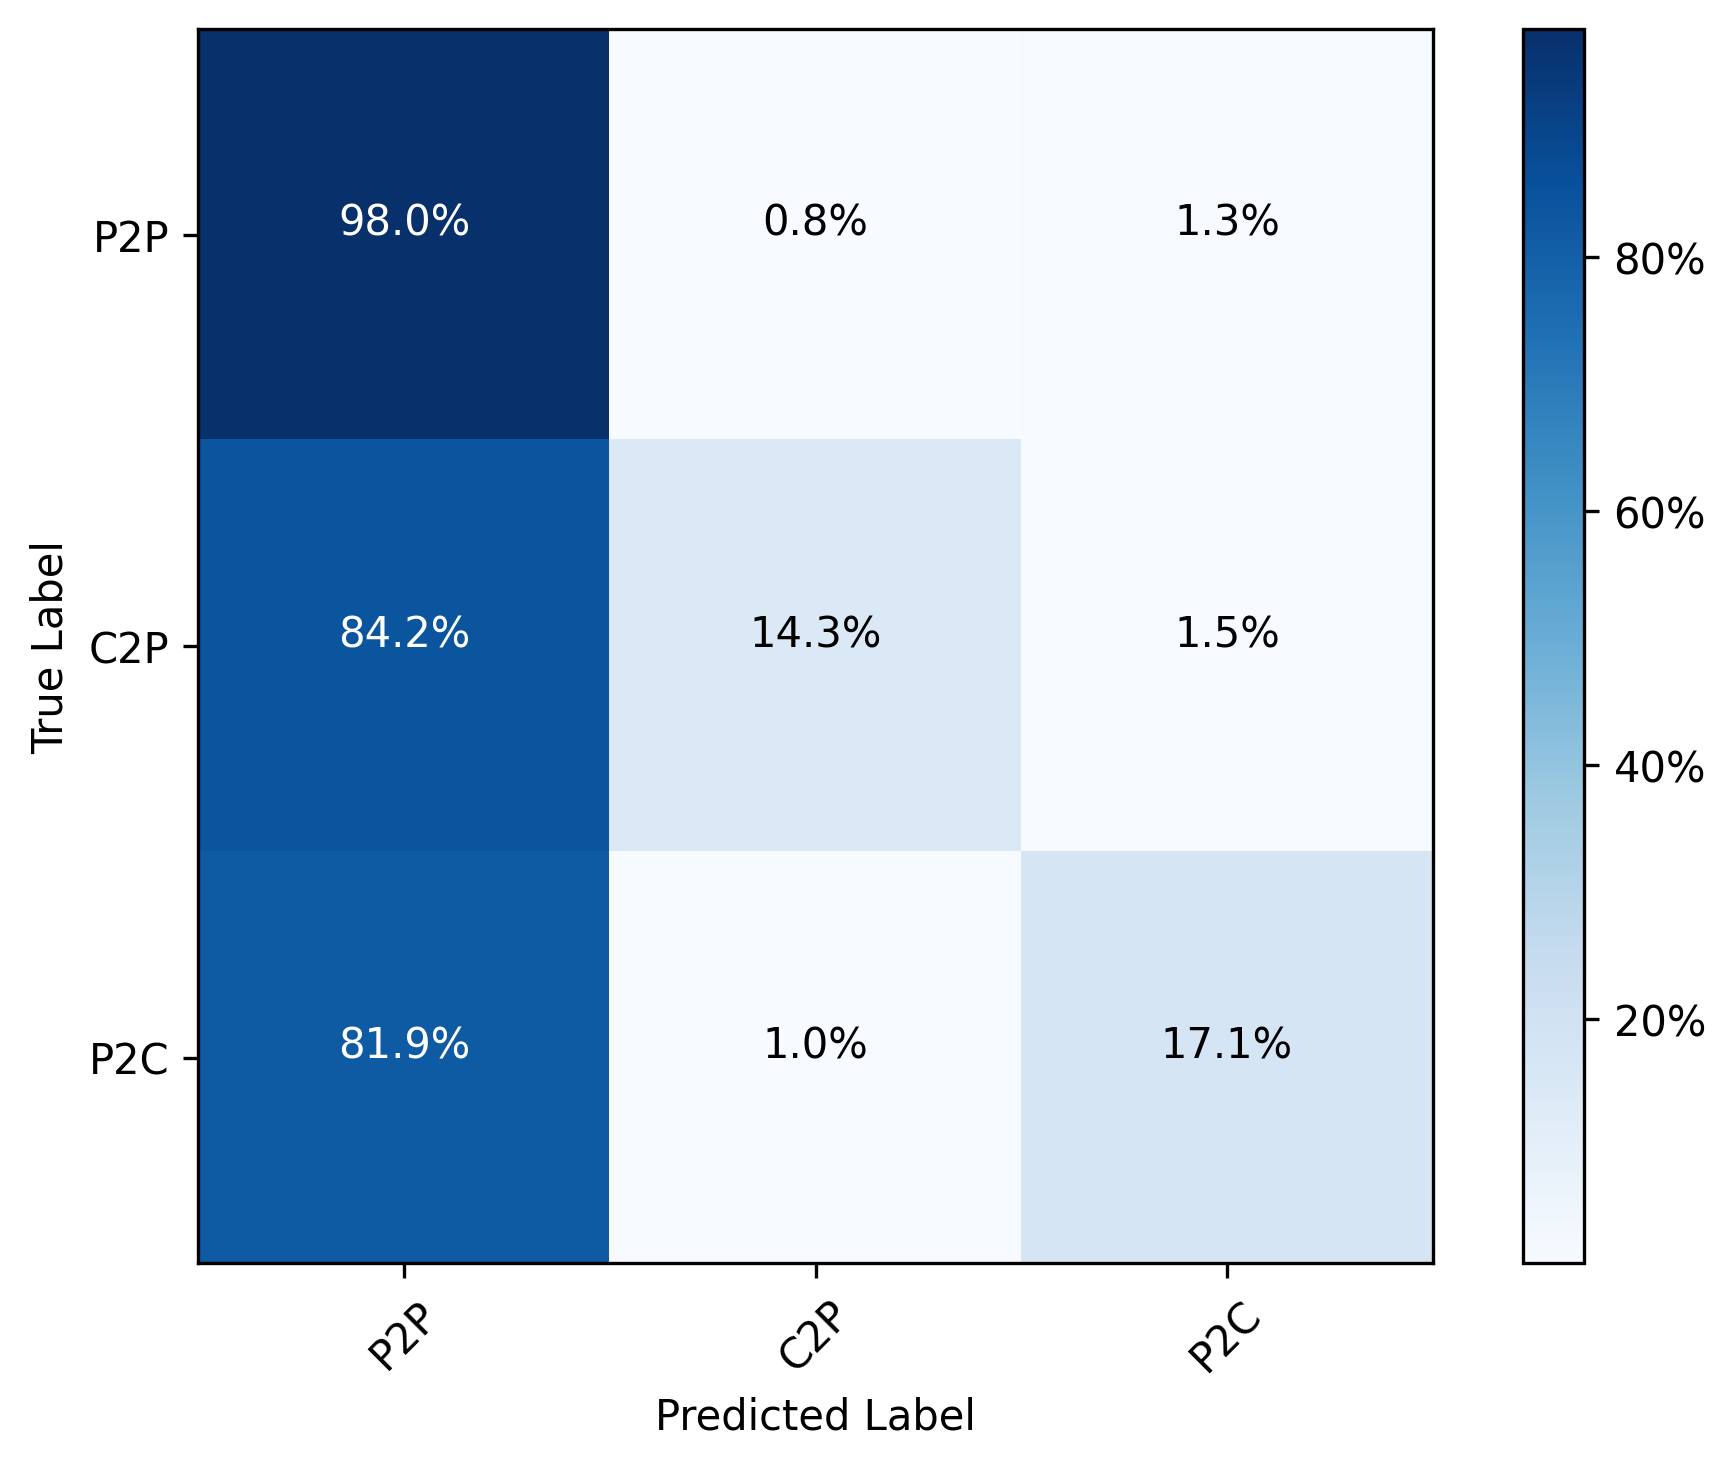
\includegraphics[width=\textwidth]{img/resultados/gnn/partes/caso1_degree/full/Confusion matrix_normalized_febrero_embeddings_ribs_DotProduct_GCN_grado_attr_febrero_with_no_batches_with_no_class_weight}
%        \caption{GCN·DP - NoBatch-NoW }
%        \label{fig:conf_matrix_gcn_dp}
%    \end{subfigure}
%    \hfill
%    \begin{subfigure}[b]{0.24\textwidth}
%        \centering
%        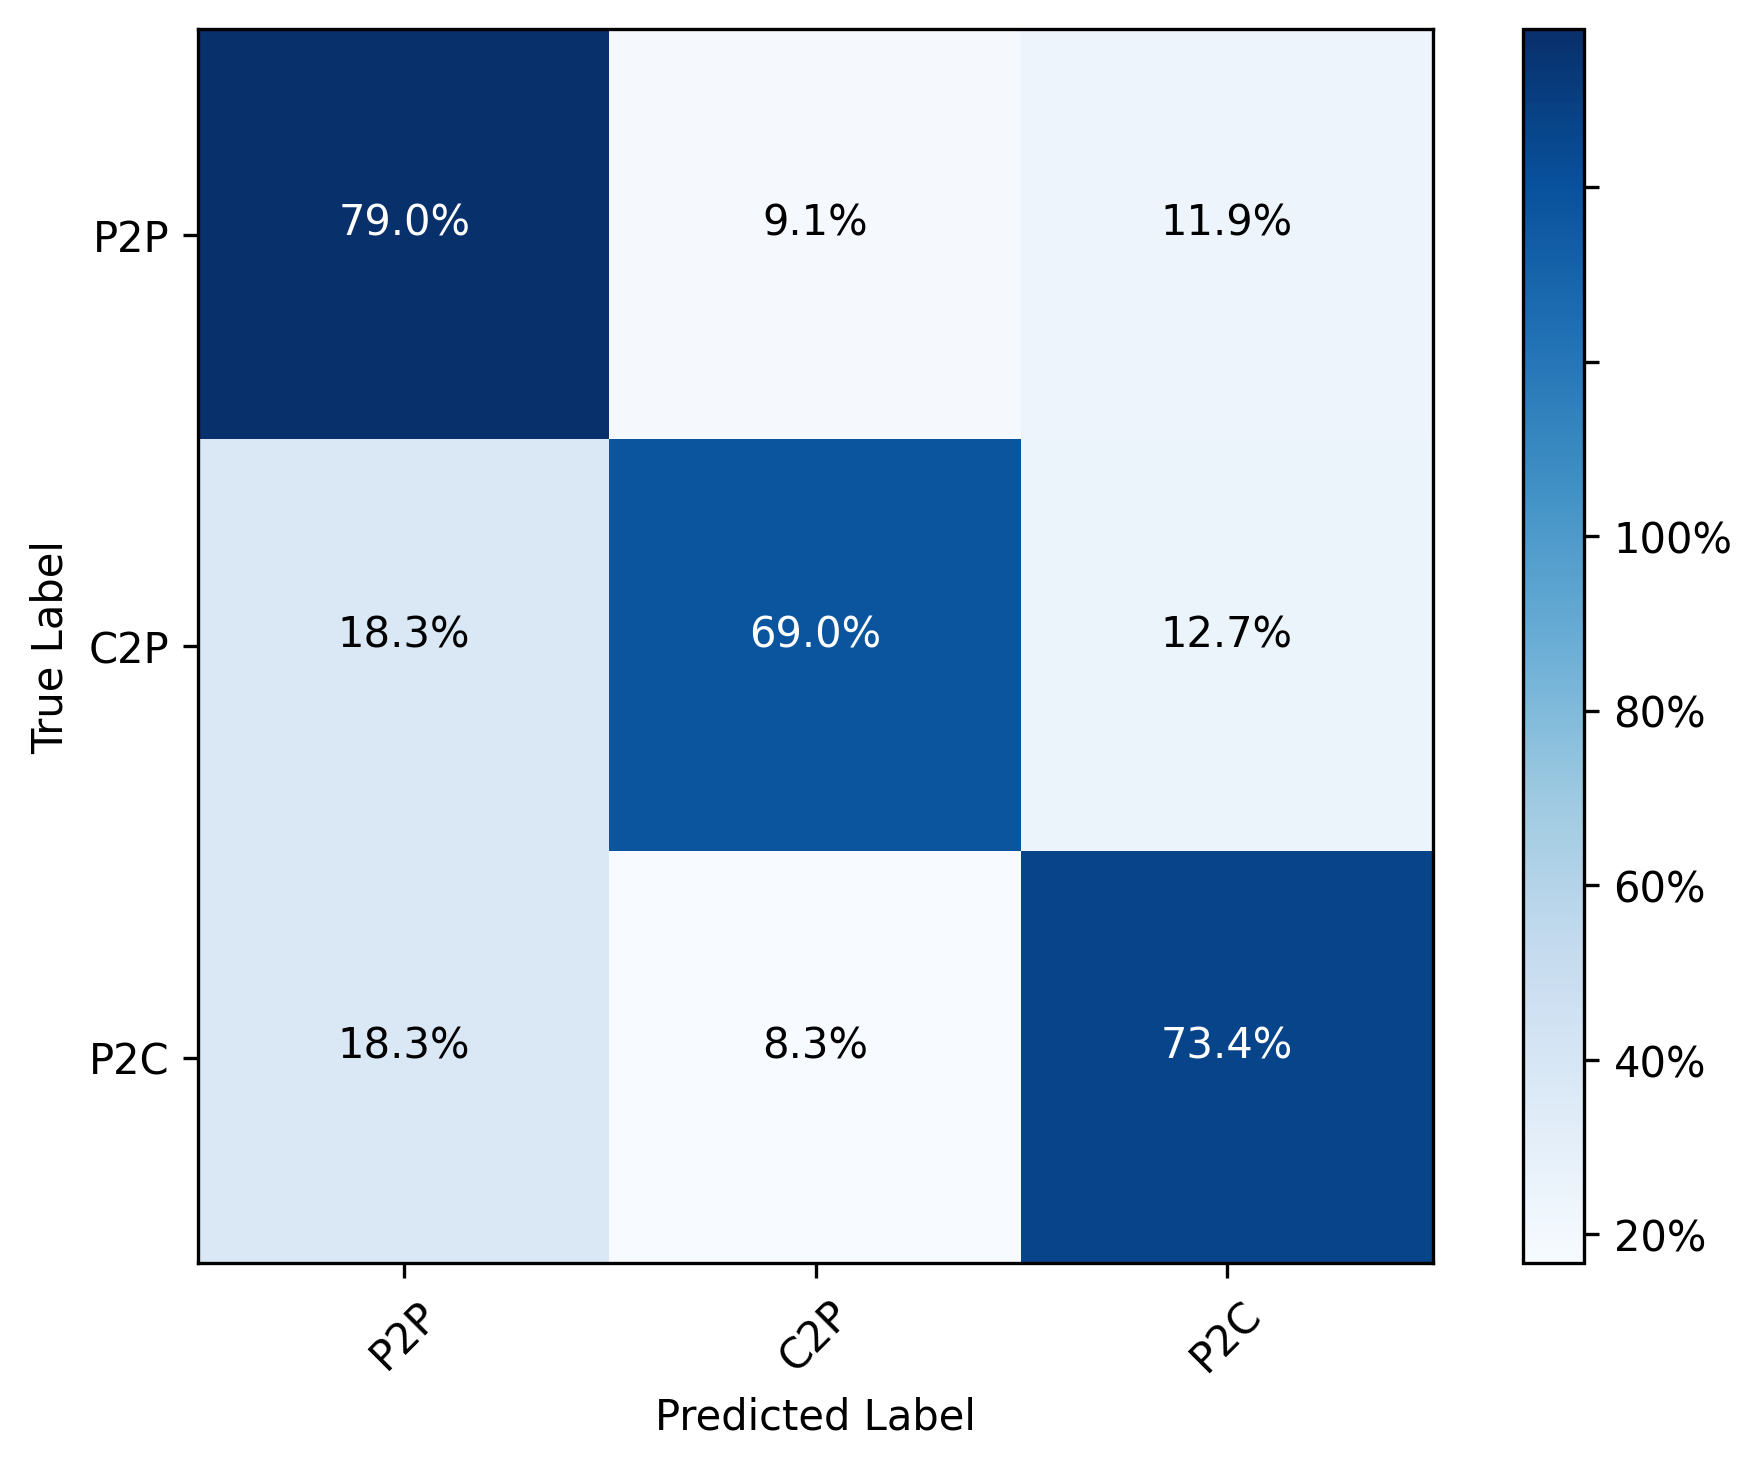
\includegraphics[width=\textwidth]{img/resultados/gnn/partes/caso1_degree/full/Confusion matrix_normalized_febrero_embeddings_ribs_DotProduct_GraphSAGE_grado_attr_febrero_with_no_batches_with_class_weight}
%        \caption{GraphSAGE·DP - NoBatch-W }
%        \label{fig:conf_matrix_sage_dp}
%    \end{subfigure}
%    \hfill
%    \begin{subfigure}[b]{0.24\textwidth}
%        \centering
%        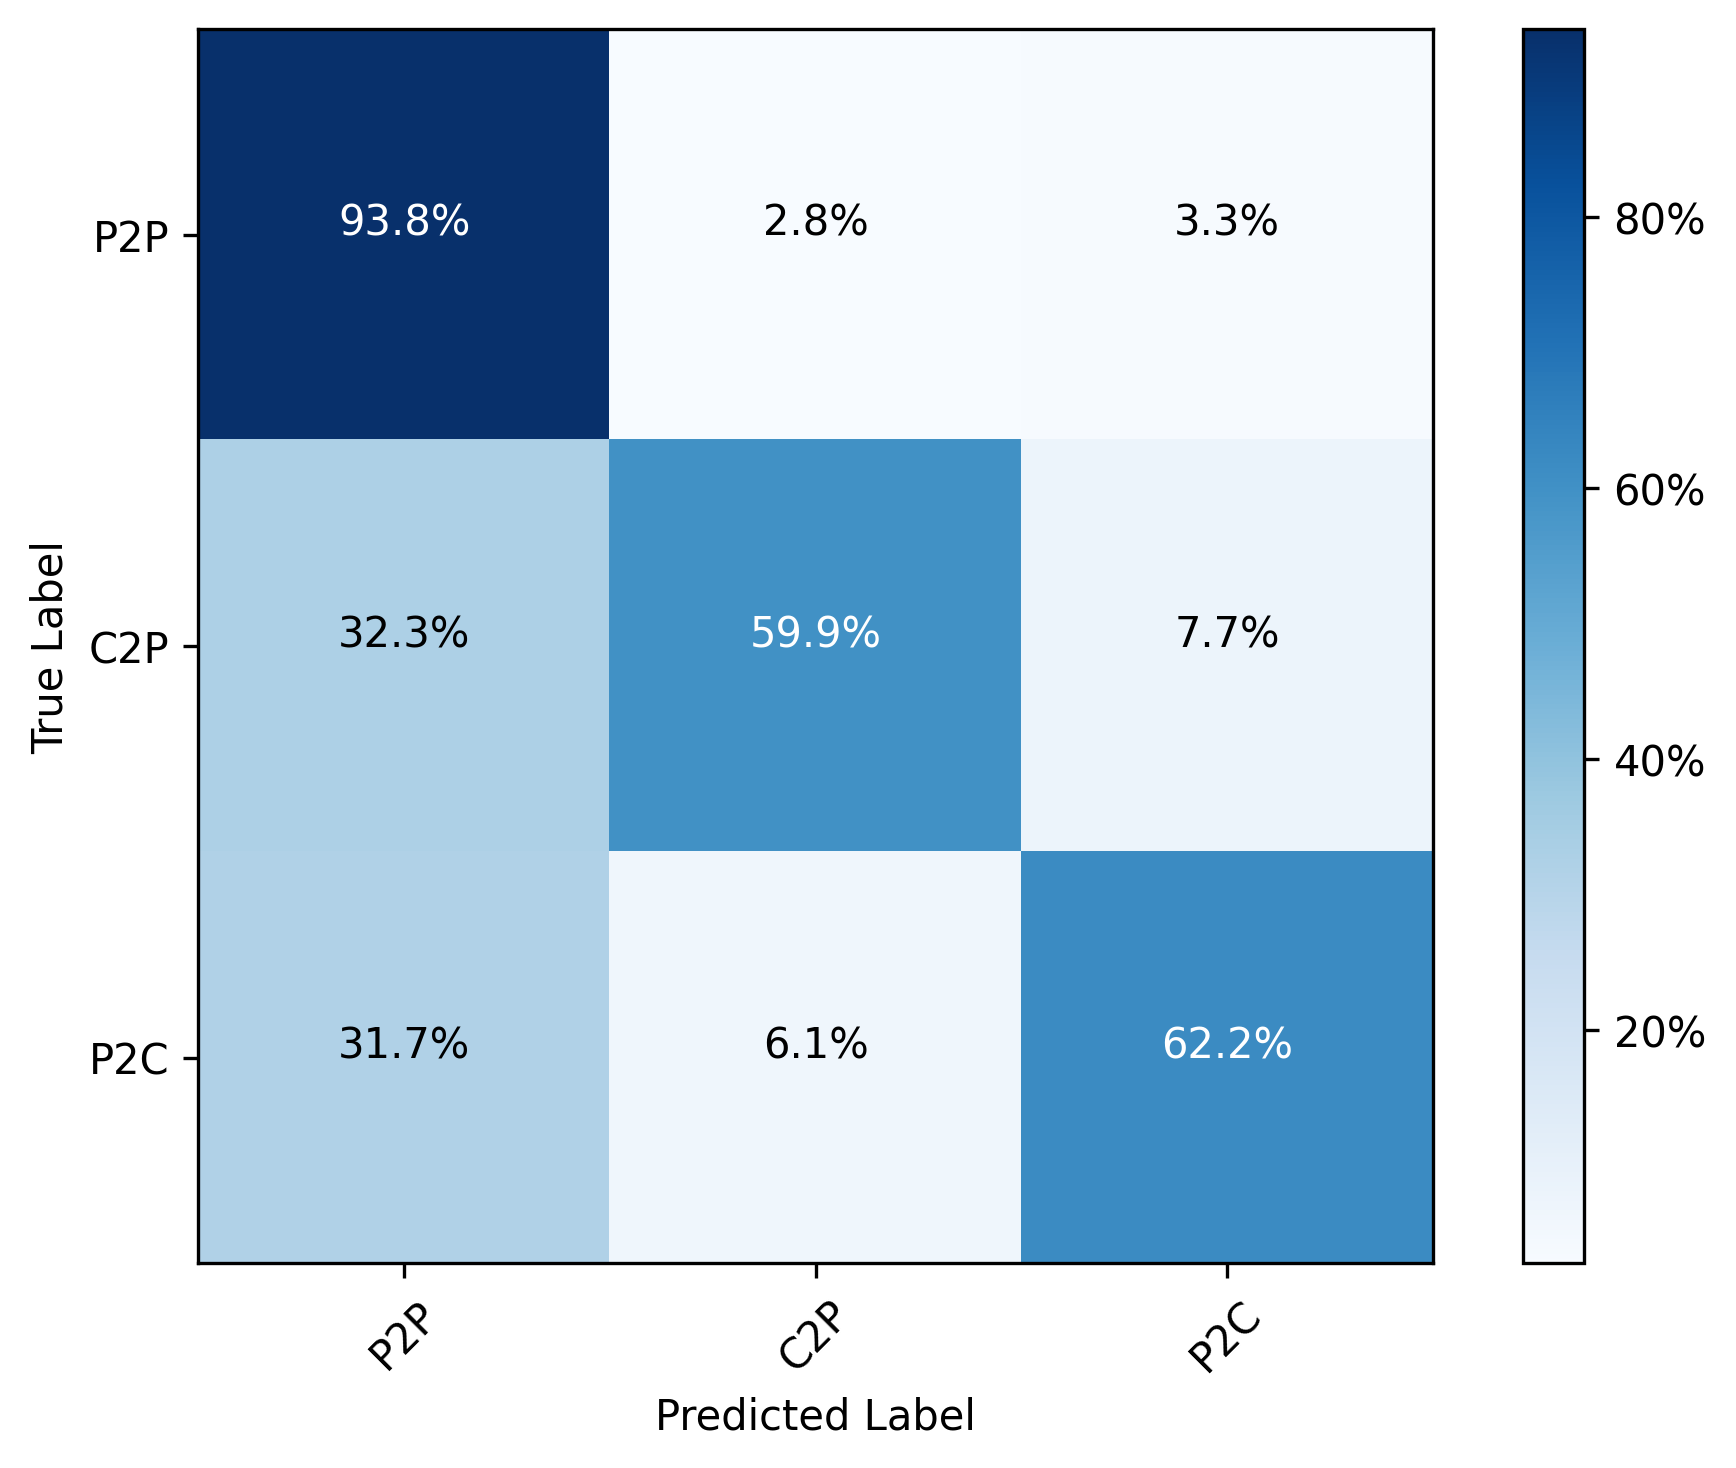
\includegraphics[width=\textwidth]{img/resultados/gnn/partes/caso1_degree/full/Confusion matrix_normalized_febrero_embeddings_ribs_DotProduct_GraphSAGE_grado_attr_febrero_with_batches_with_no_class_weight}
%        \caption{GCN·DP - Batch-NoW }
%        \label{fig:conf_matrix_gat_dp}
%    \end{subfigure}
%    \hfill
%    \begin{subfigure}[b]{0.24\textwidth}
%        \centering
%        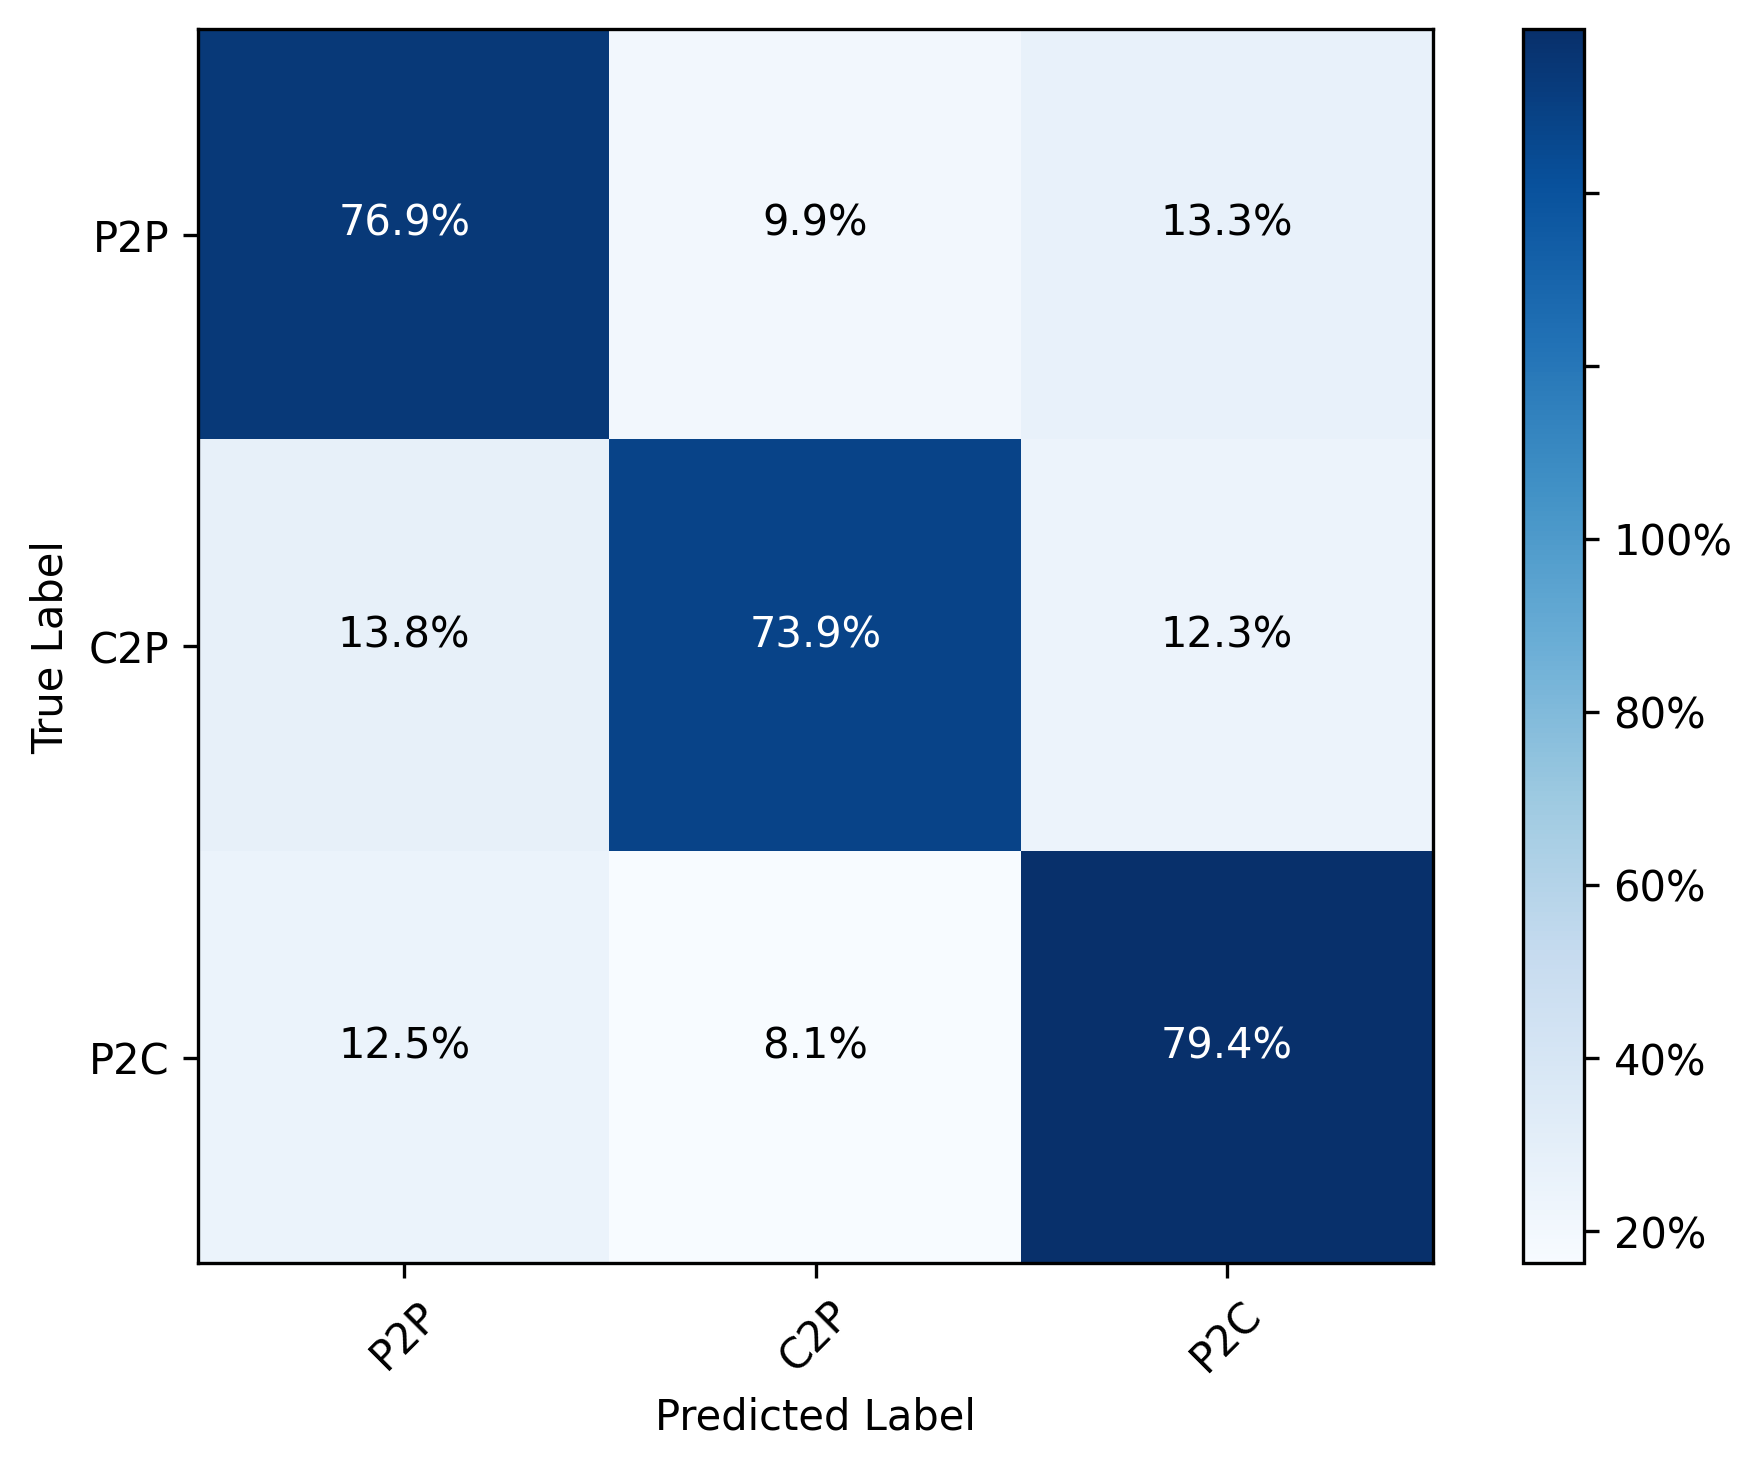
\includegraphics[width=\textwidth]{img/resultados/gnn/partes/caso1_degree/full/Confusion matrix_normalized_febrero_embeddings_ribs_DotProduct_GraphSAGE_grado_attr_febrero_with_batches_with_class_weight}
%        \caption{GCN·DP - Batch-W }
%        \label{fig:conf_matrix_gat_dp}
%    \end{subfigure}
%
%
%
    %\caption{}
%    \label{fig:muchas_mc_enfoqueporpartes}
%\end{figure}
%
%\begin{figure}[H]
%    \centering
%    \vspace{0.5cm}
%    % Tercera fila ///////////////////////////////////////////////
%    \begin{subfigure}[b]{0.24\textwidth}
%        \centering
%        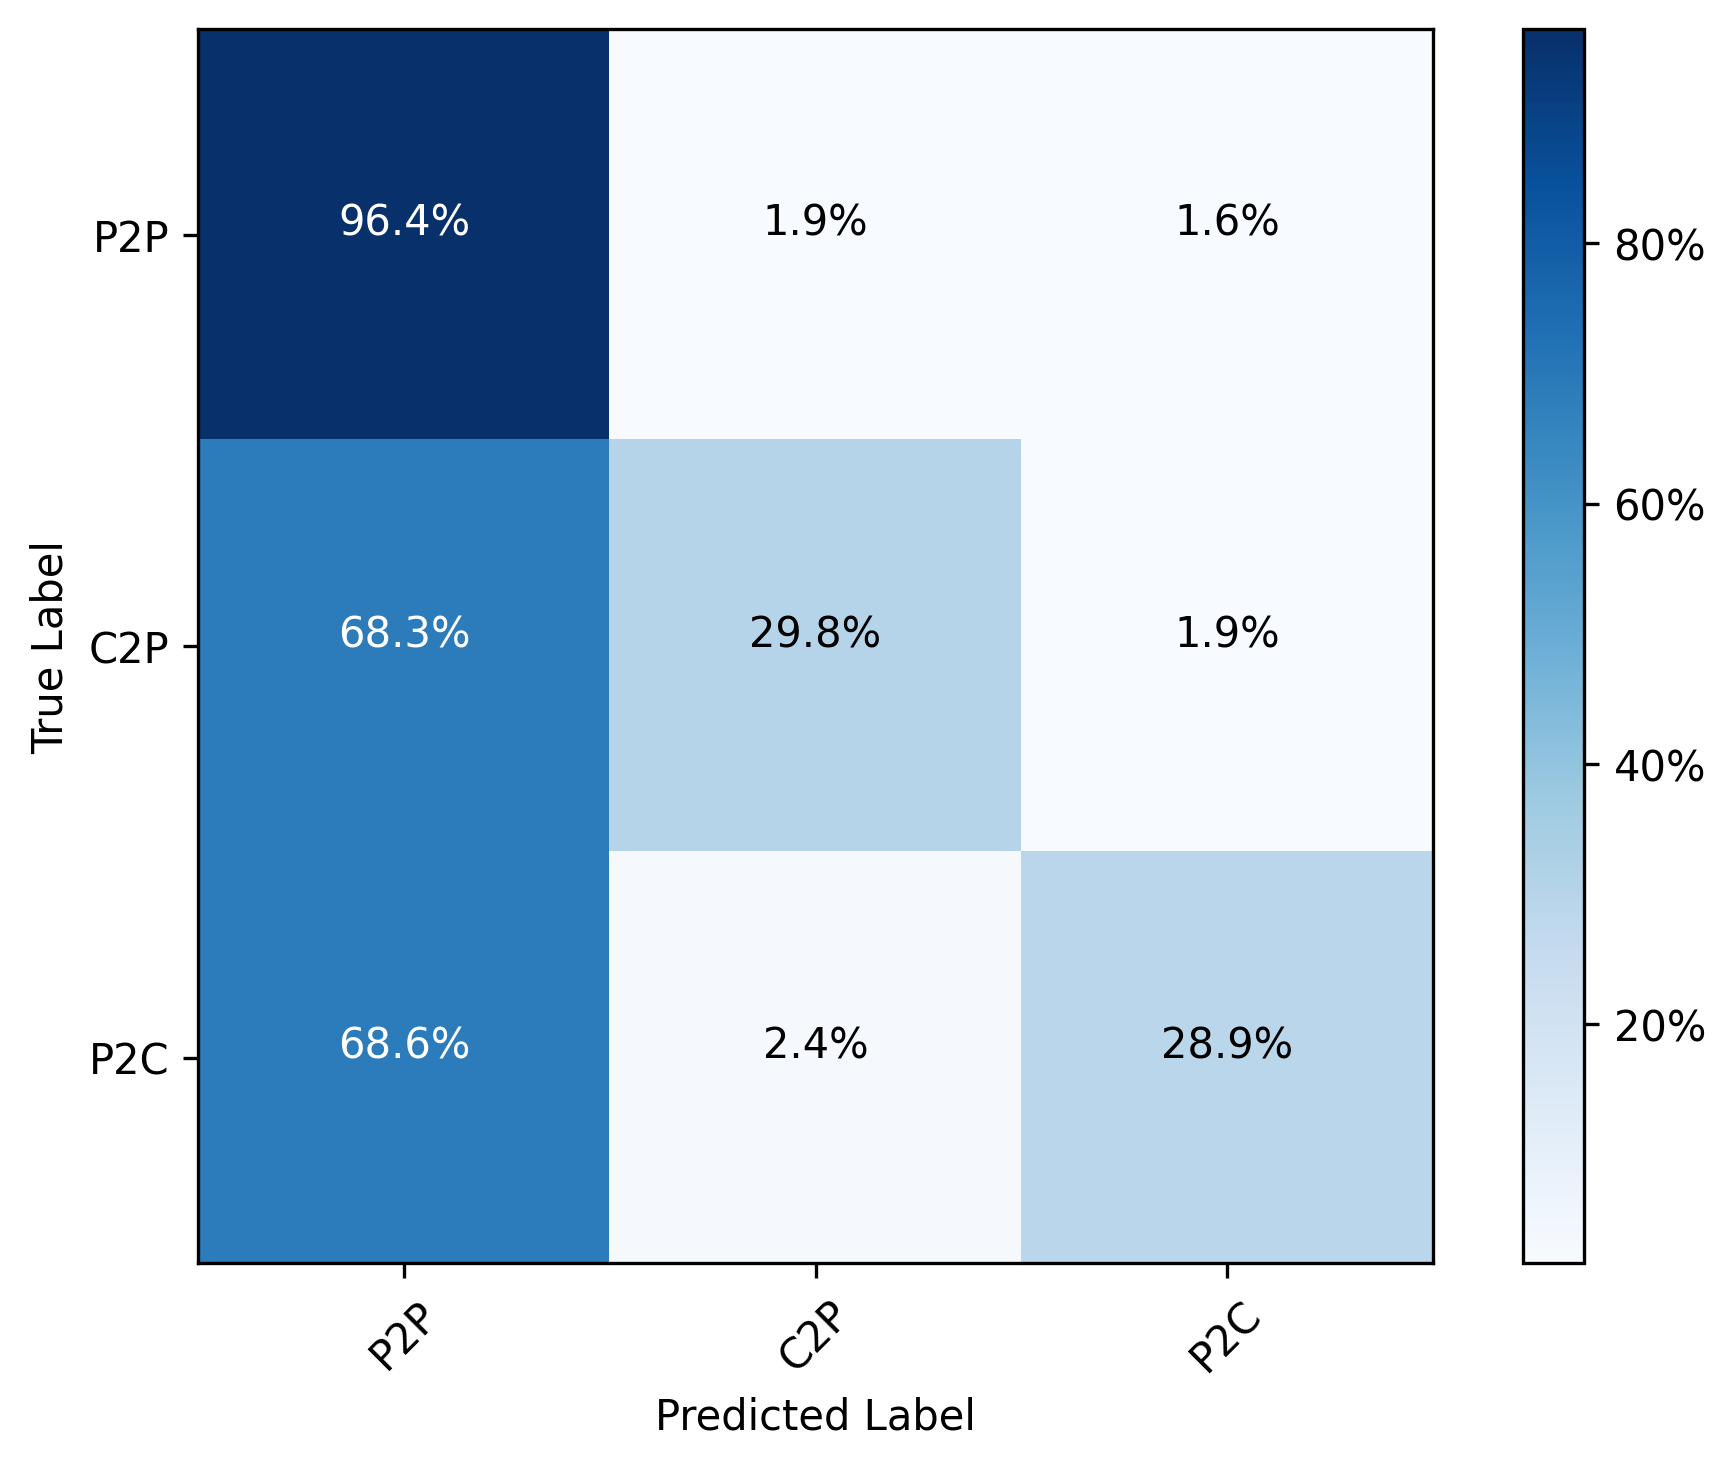
\includegraphics[width=\textwidth]{img/resultados/gnn/partes/caso1_degree/full/Confusion matrix_normalized_febrero_embeddings_ribs_DotProduct_GAT_grado_attr_febrero_with_no_batches_with_no_class_weight}
%        \caption{GAT·DP - NoBatch-NoW }
%        \label{fig:conf_matrix_gcn_dp}
%    \end{subfigure}
%    \hfill
%    \begin{subfigure}[b]{0.24\textwidth}
%        \centering
%        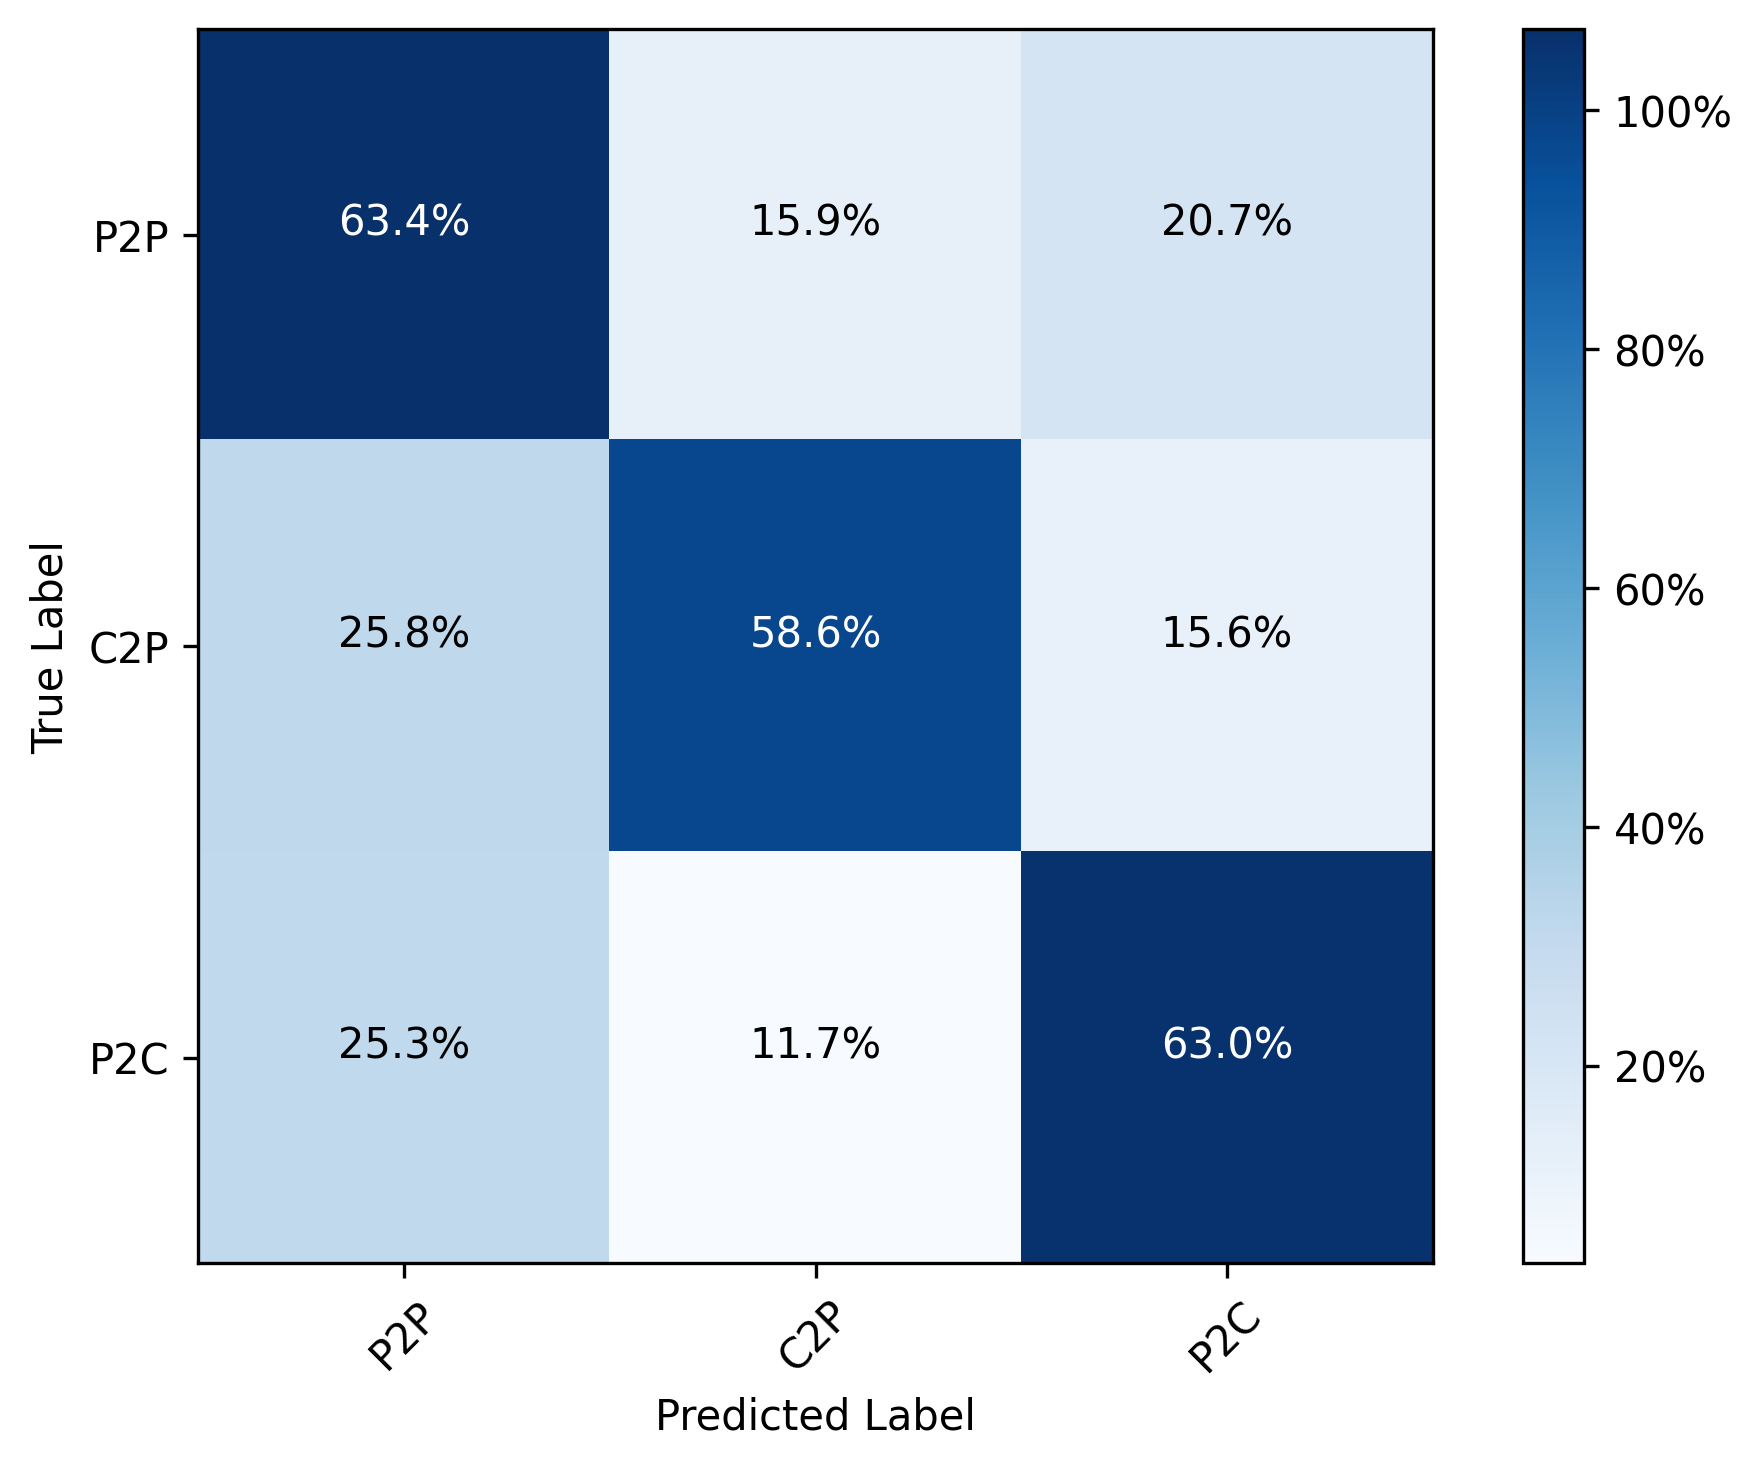
\includegraphics[width=\textwidth]{img/resultados/gnn/partes/caso1_degree/full/Confusion matrix_normalized_febrero_embeddings_ribs_DotProduct_GAT_grado_attr_febrero_with_no_batches_with_class_weight}
%        \caption{GAT·DP - NoBatch-W}
%        \label{fig:conf_matrix_sage_dp}
%    \end{subfigure}
%    \hfill
%    \begin{subfigure}[b]{0.24\textwidth}
%        \centering
%        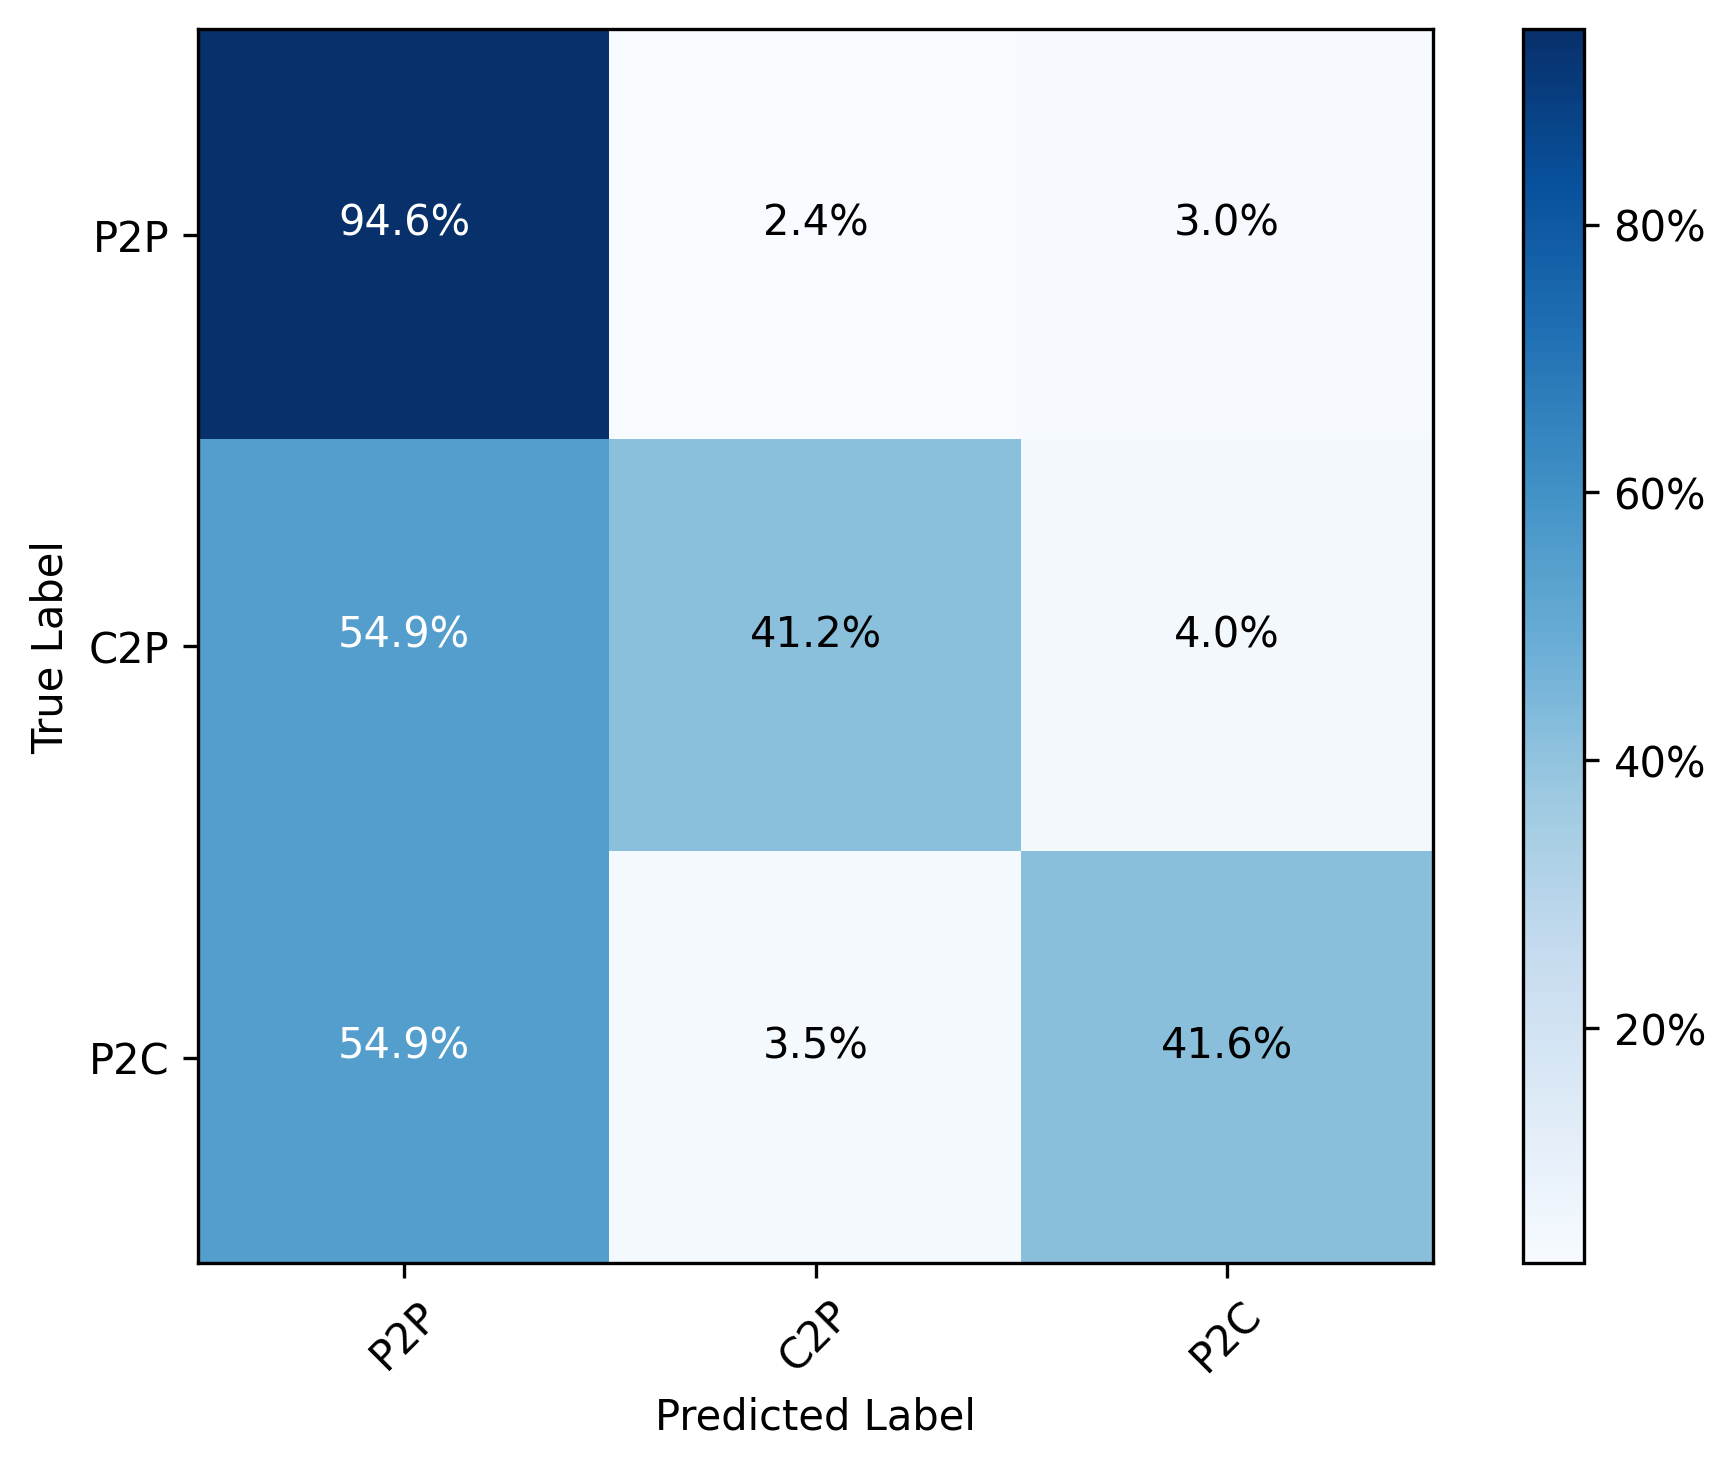
\includegraphics[width=\textwidth]{img/resultados/gnn/partes/caso1_degree/full/Confusion matrix_normalized_febrero_embeddings_ribs_DotProduct_GAT_grado_attr_febrero_with_batches_with_no_class_weight}
%        \caption{GAT·DP - Batch-NoW }
%        \label{fig:conf_matrix_gat_dp}
%    \end{subfigure}
%    \hfill
%    \begin{subfigure}[b]{0.24\textwidth}
%        \centering
%        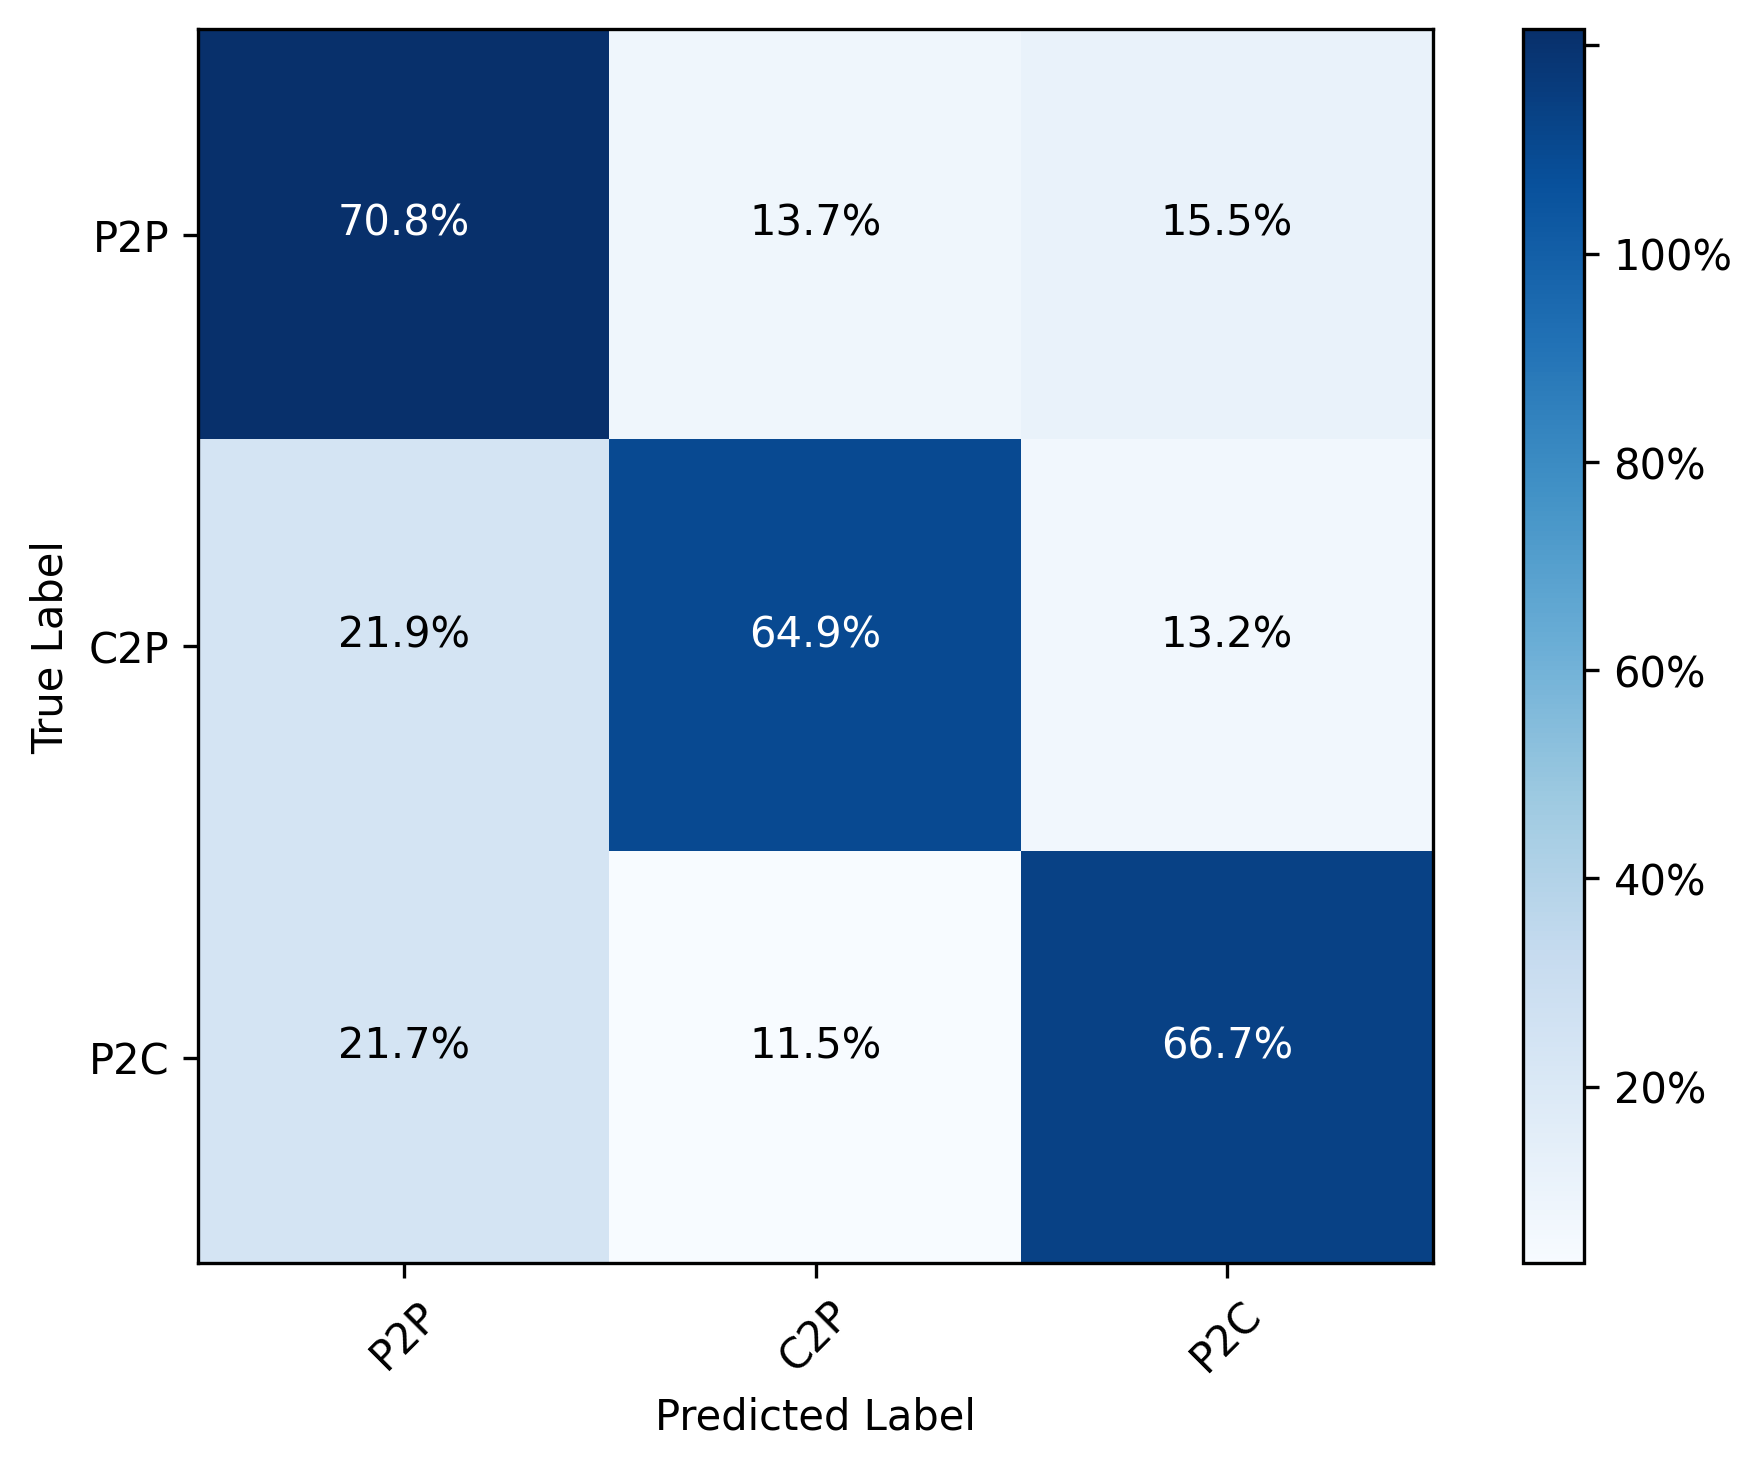
\includegraphics[width=\textwidth]{img/resultados/gnn/partes/caso1_degree/full/Confusion matrix_normalized_febrero_embeddings_ribs_DotProduct_GAT_grado_attr_febrero_with_batches_with_class_weight}
%        \caption{GAT·DP - Batch-W }
%        \label{fig:conf_matrix_gat_dp}
%    \end{subfigure}
%
%    %\label{fig:...}
%\end{figure}
%
%\begin{figure}[H]
%    \centering
%% Cuarta fila ///////////////////////////////////////////////////
%    \begin{subfigure}[b]{0.24\textwidth}
%        \centering
%        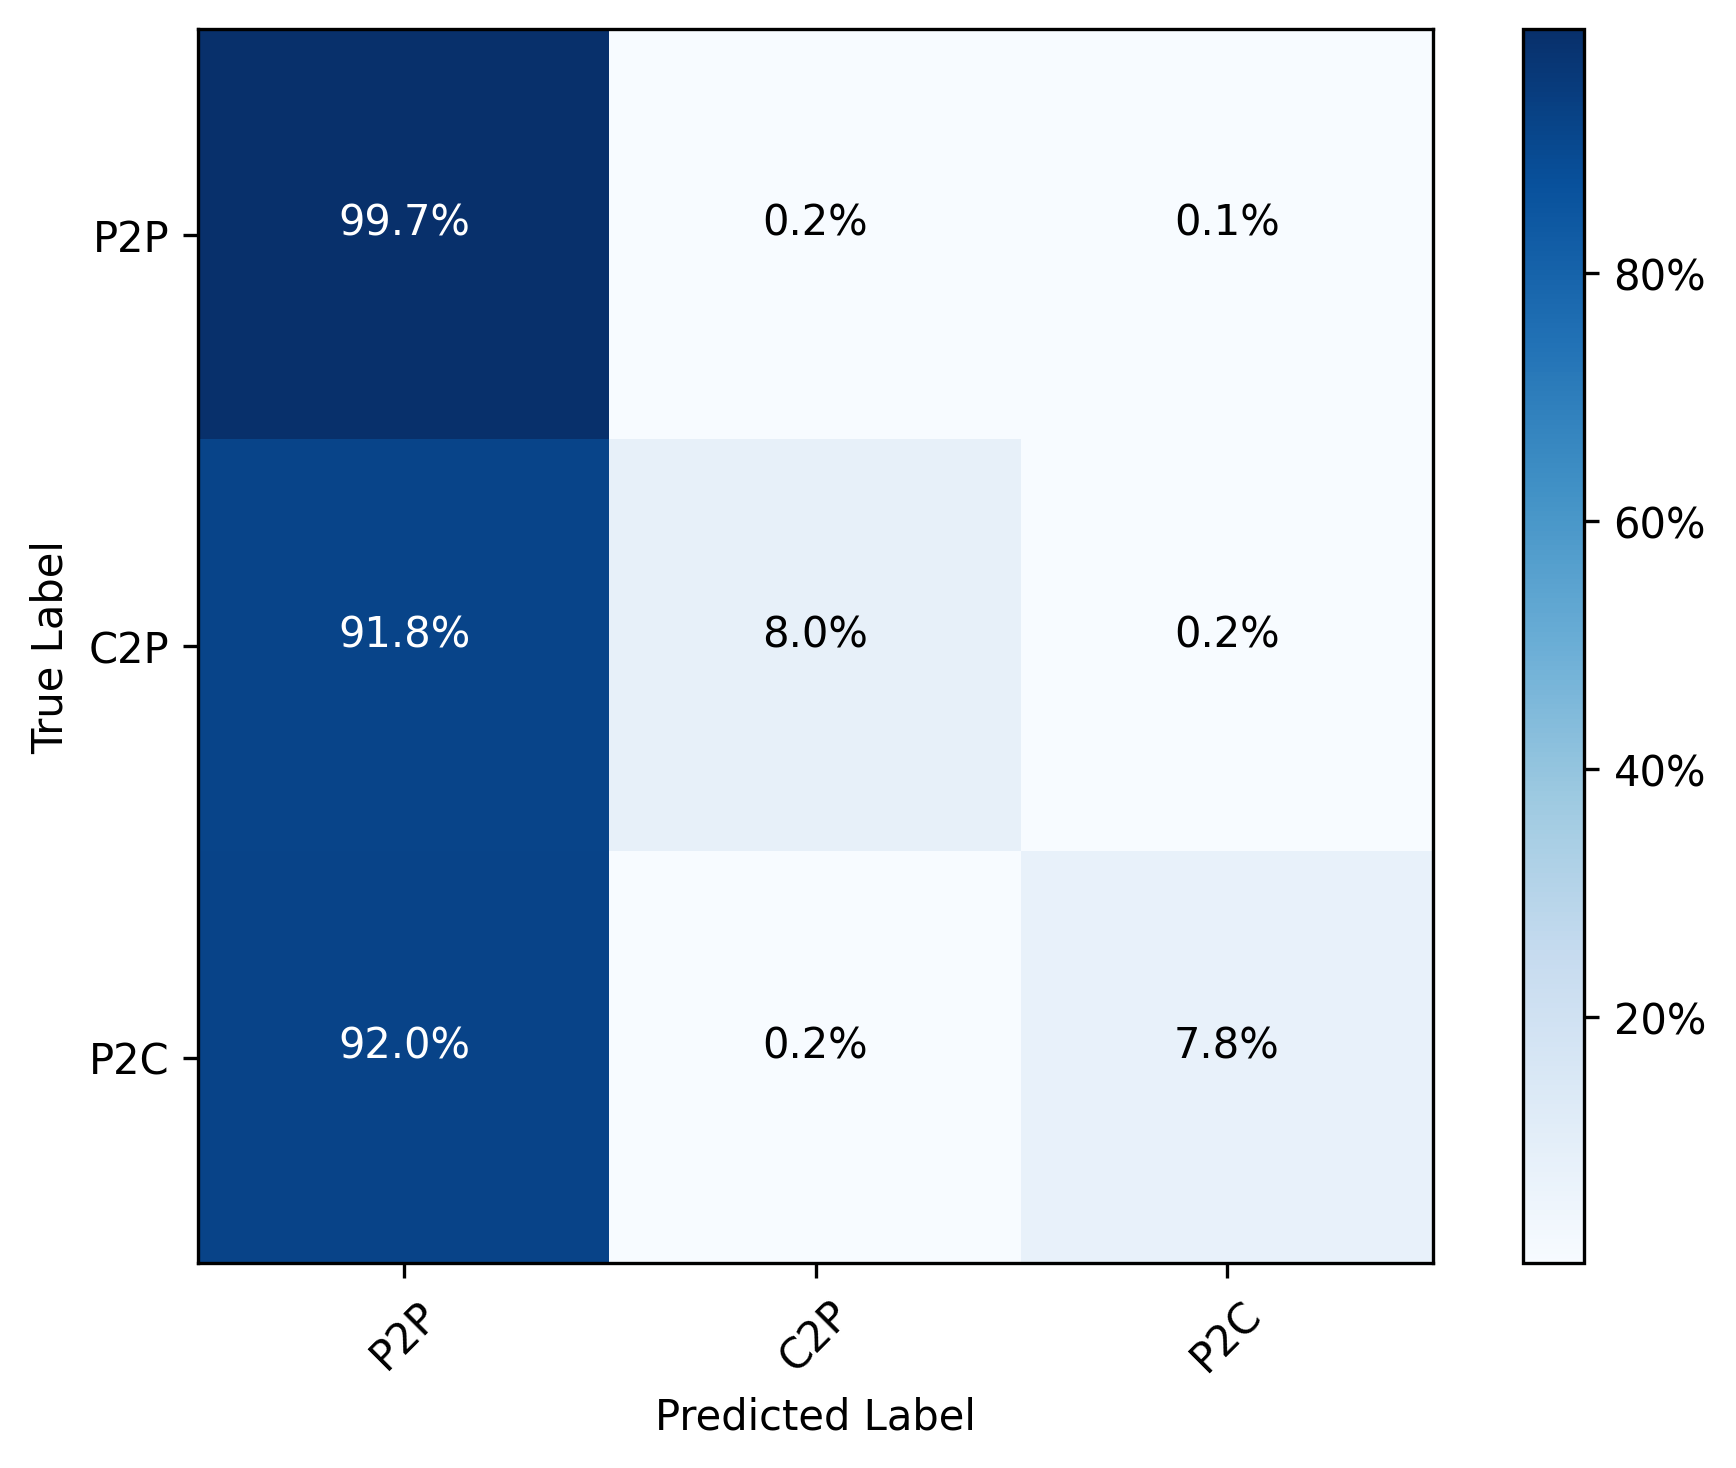
\includegraphics[width=\textwidth]{img/resultados/gnn/partes/caso1_degree/full/Confusion matrix_normalized_febrero_embeddings_ribs_MLP_GCN_grado_attr_febrero_with_no_batches_with_no_class_weight}
%        \caption{GCN·MLP - NoBatch-NoW }
%        \label{fig:conf_matrix_gcn_dp}
%    \end{subfigure}
%    \hfill
%    \begin{subfigure}[b]{0.24\textwidth}
%        \centering
%        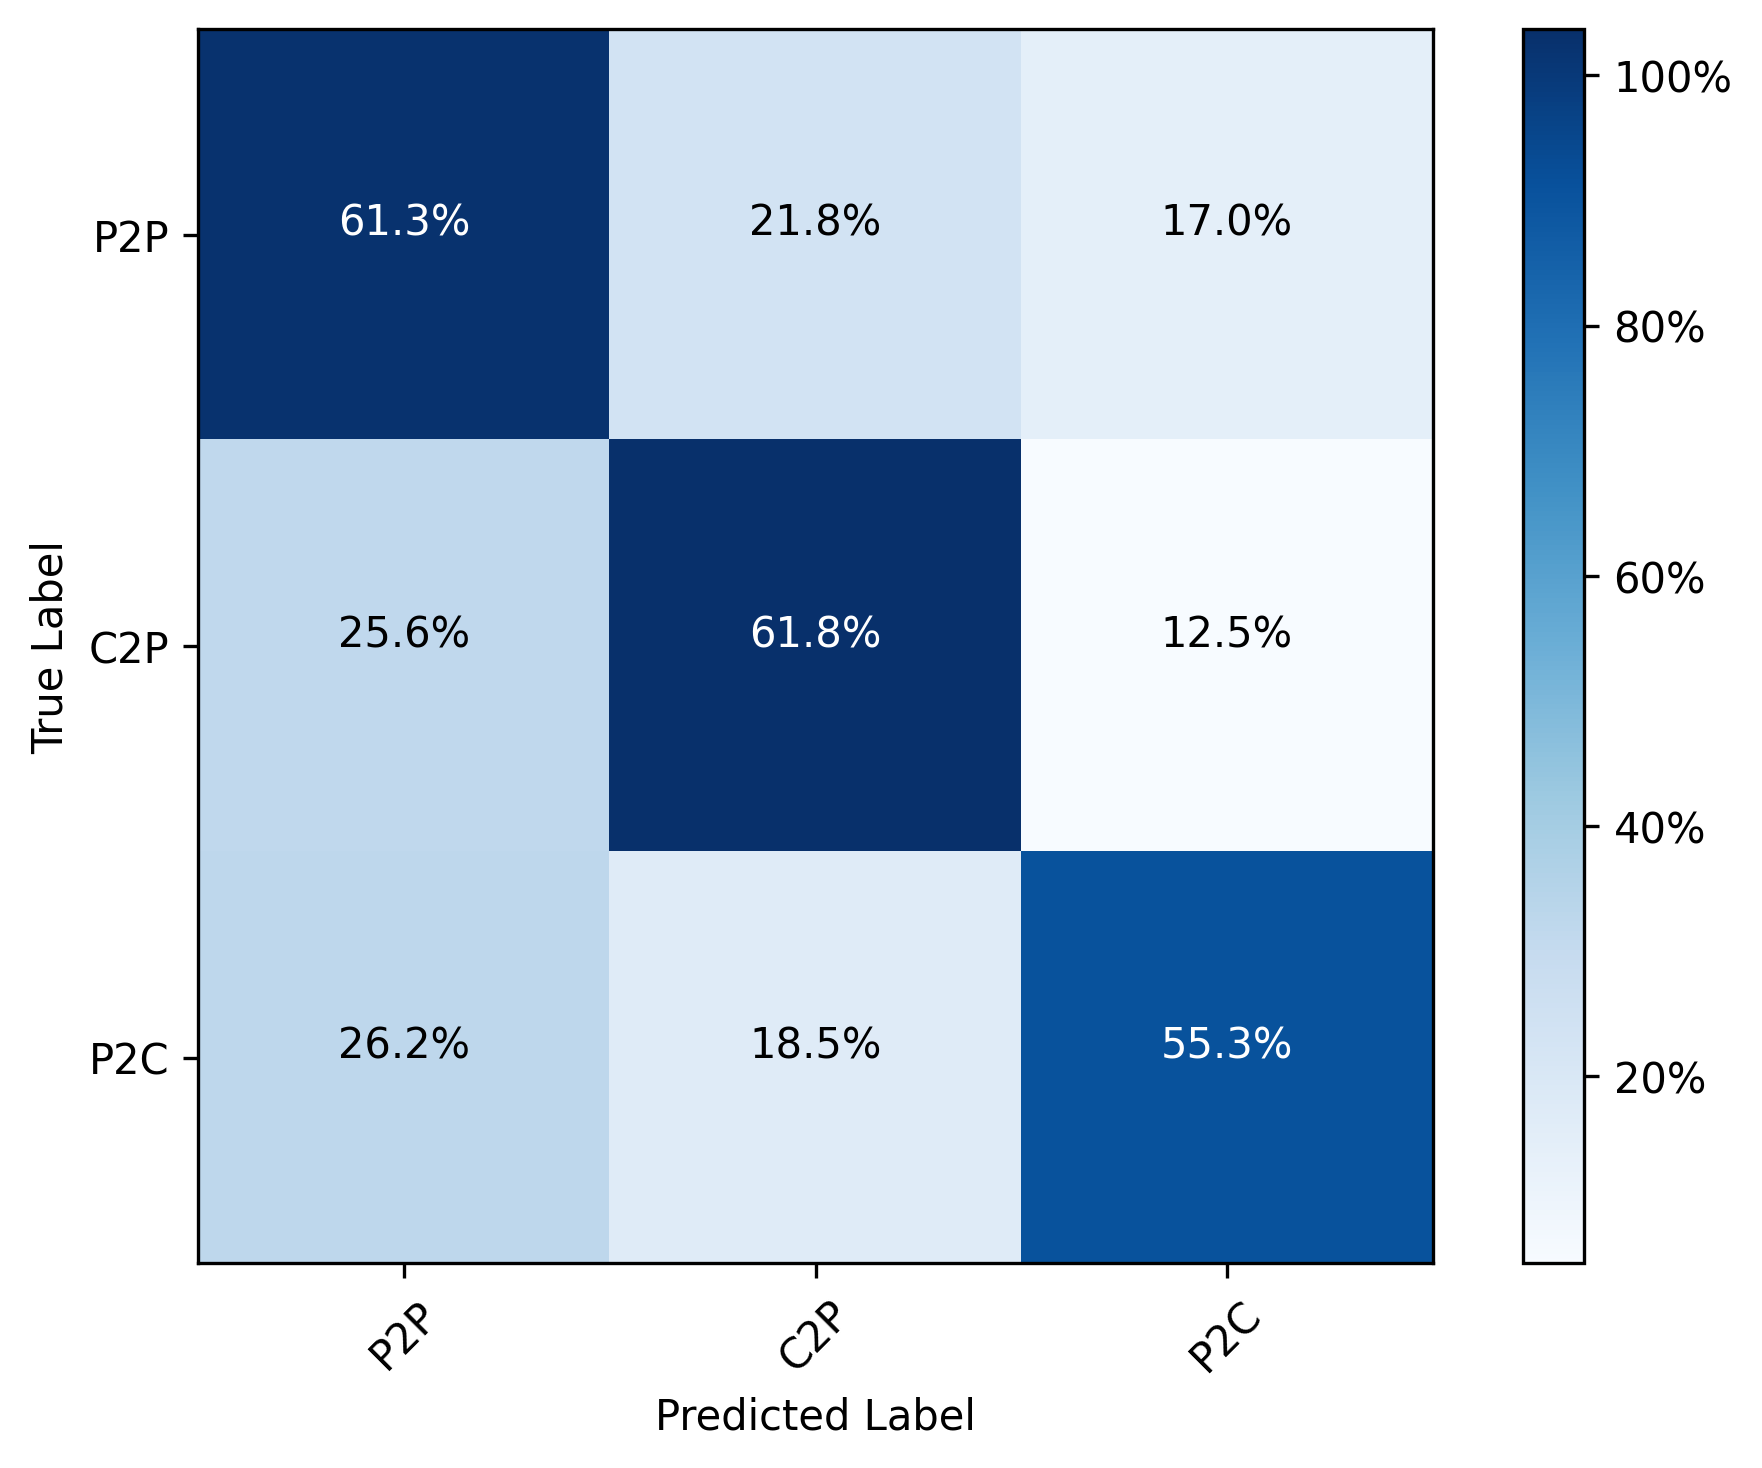
\includegraphics[width=\textwidth]{img/resultados/gnn/partes/caso1_degree/full/Confusion matrix_normalized_febrero_embeddings_ribs_MLP_GCN_grado_attr_febrero_with_no_batches_with_class_weight}
%        \caption{GCN·MLP - NoBatch-W}
%        \label{fig:conf_matrix_sage_dp}
%    \end{subfigure}
%    \hfill
%    \begin{subfigure}[b]{0.24\textwidth}
%        \centering
%        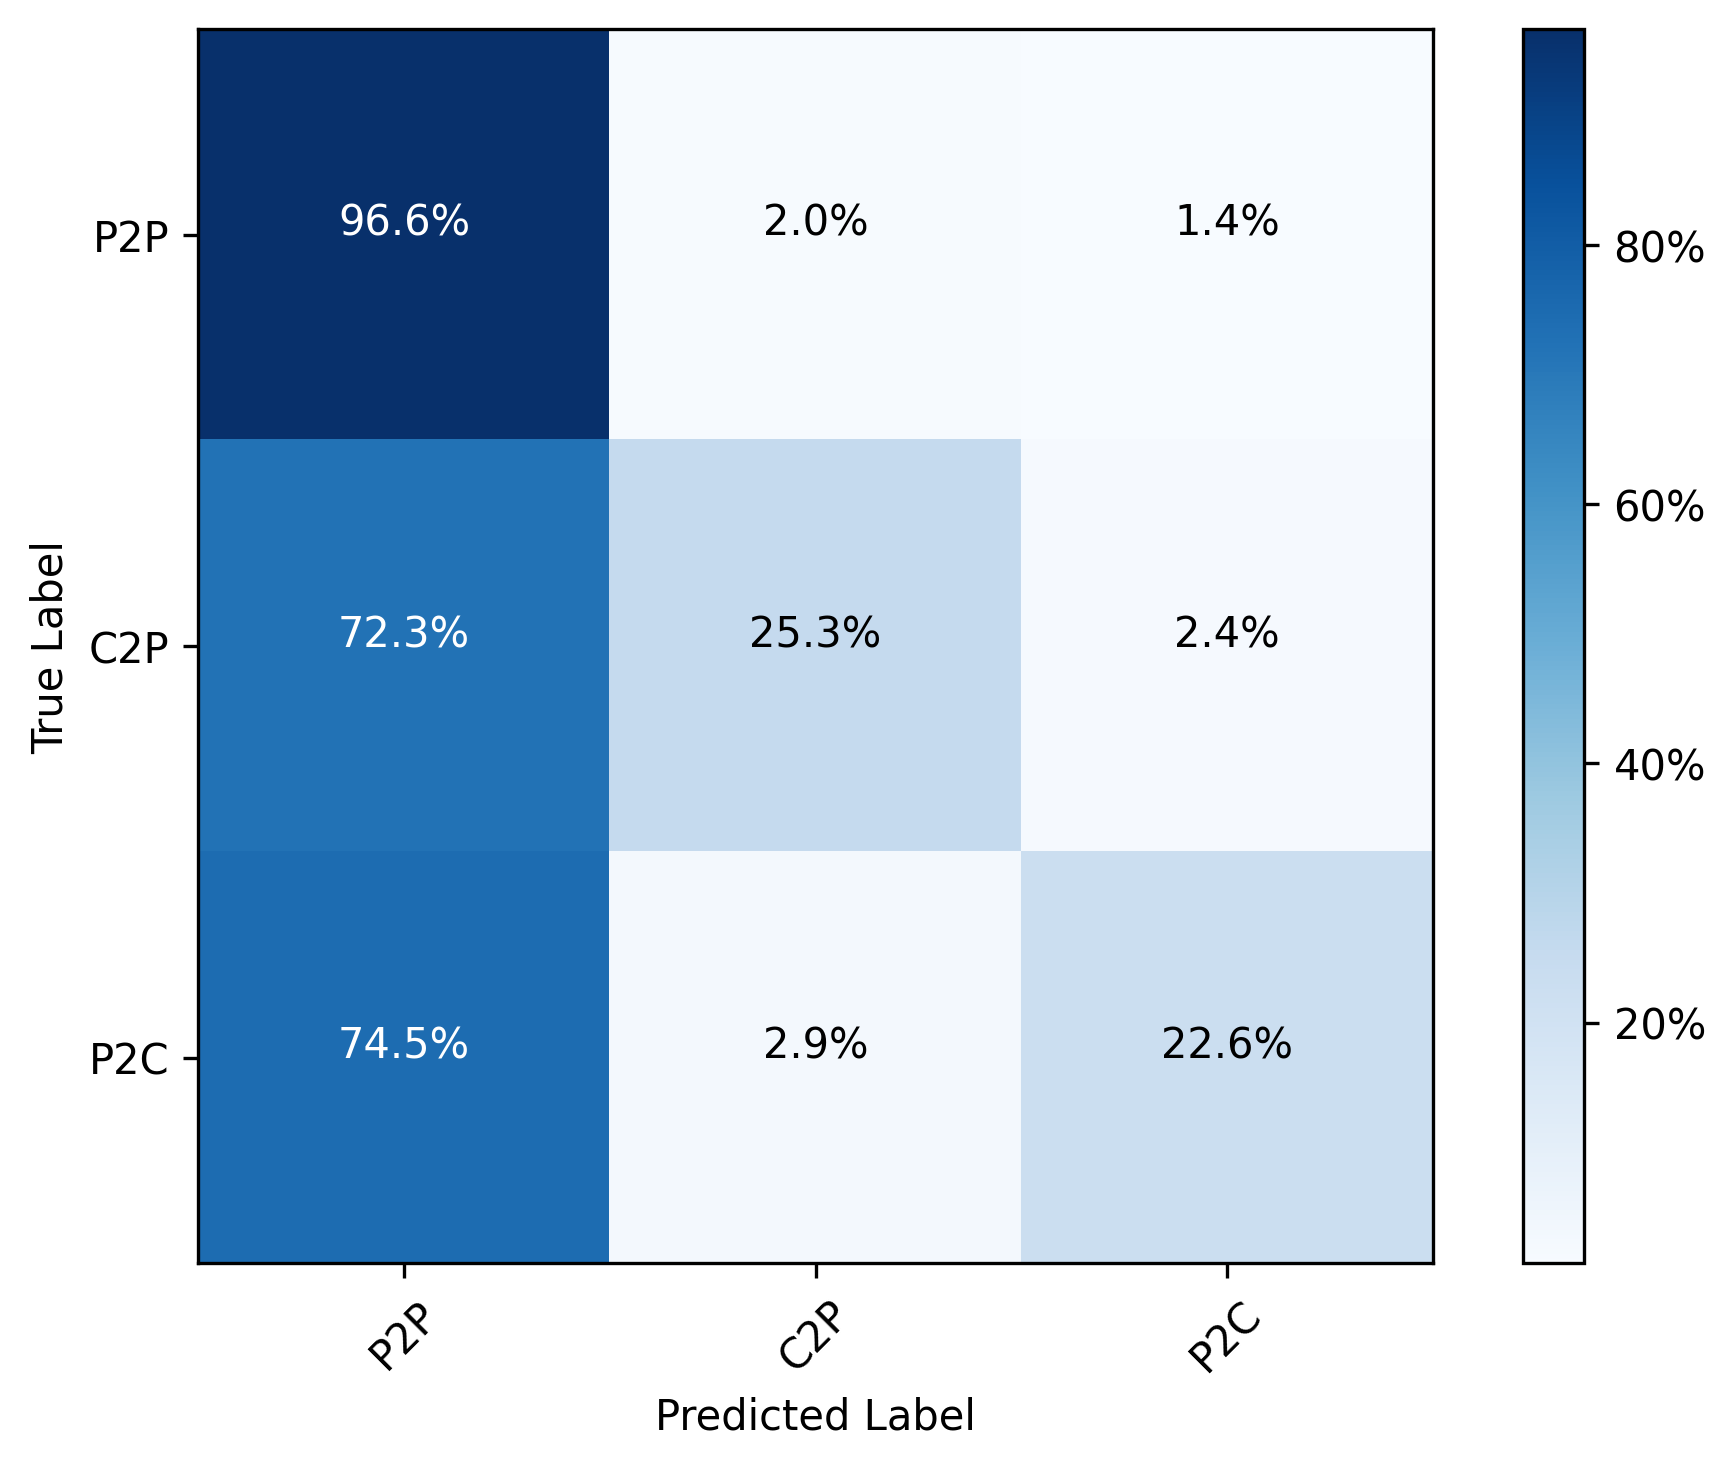
\includegraphics[width=\textwidth]{img/resultados/gnn/partes/caso1_degree/full/Confusion matrix_normalized_febrero_embeddings_ribs_MLP_GCN_grado_attr_febrero_with_batches_with_no_class_weight}
%        \caption{GCN·MLP - Batch-NoW }
%        \label{fig:conf_matrix_gat_dp}
%    \end{subfigure}
%    \hfill
%    \begin{subfigure}[b]{0.24\textwidth}
%        \centering
%        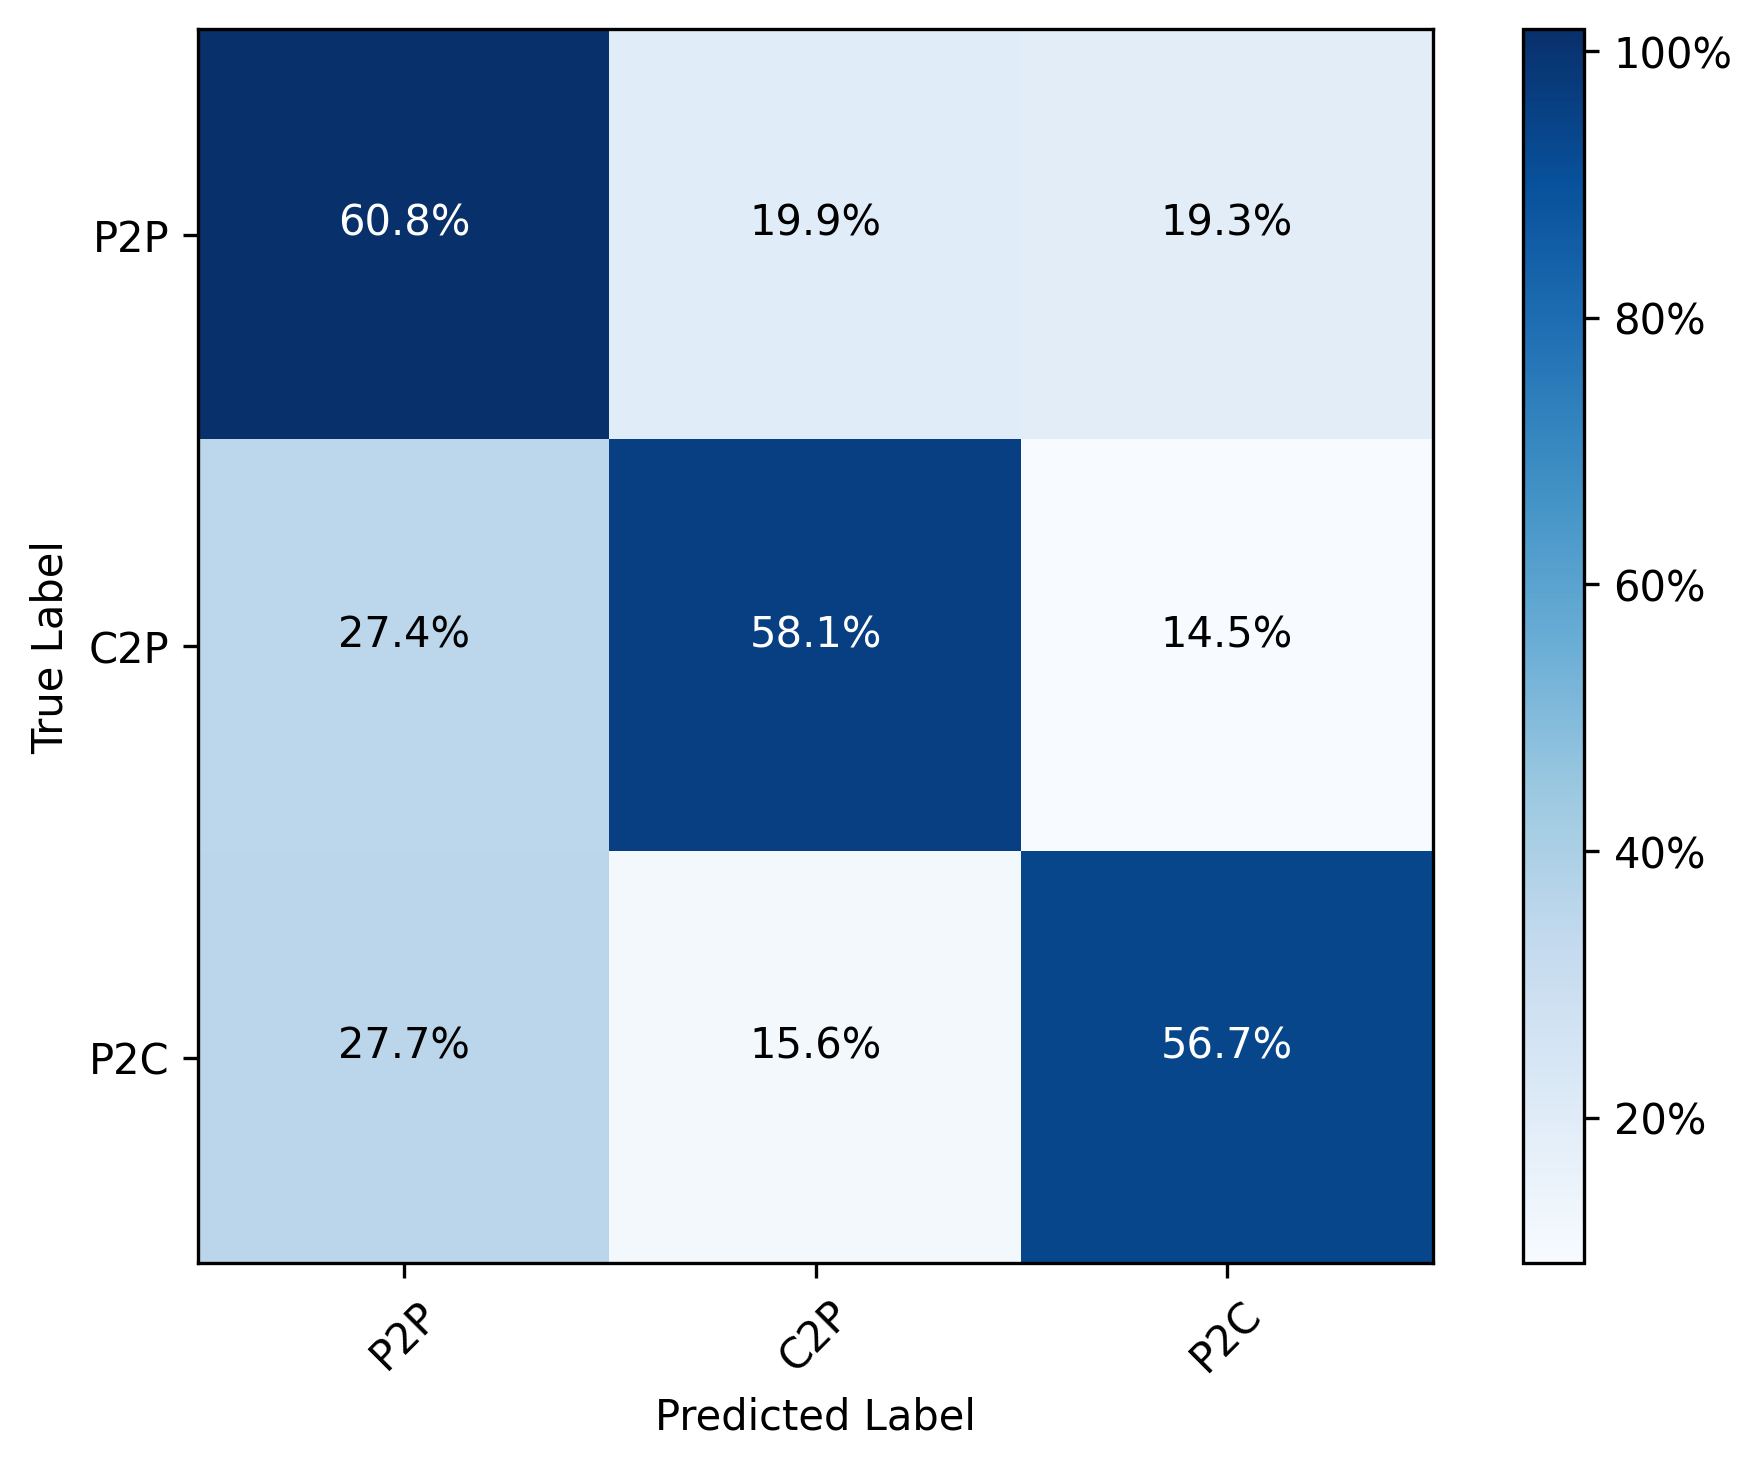
\includegraphics[width=\textwidth]{img/resultados/gnn/partes/caso1_degree/full/Confusion matrix_normalized_febrero_embeddings_ribs_MLP_GCN_grado_attr_febrero_with_batches_with_class_weight}
%        \caption{GCN·MLP - Batch-W  }
%        \label{fig:conf_matrix_gat_dp}
%    \end{subfigure}
    %\caption{}   
%\end{figure}
%\begin{figure}[H]
%    \centering
%    %QUINTA FILA: GraphSAGE MLP//////////////////////////////
%        \begin{subfigure}[b]{0.24\textwidth}
%        \centering
%        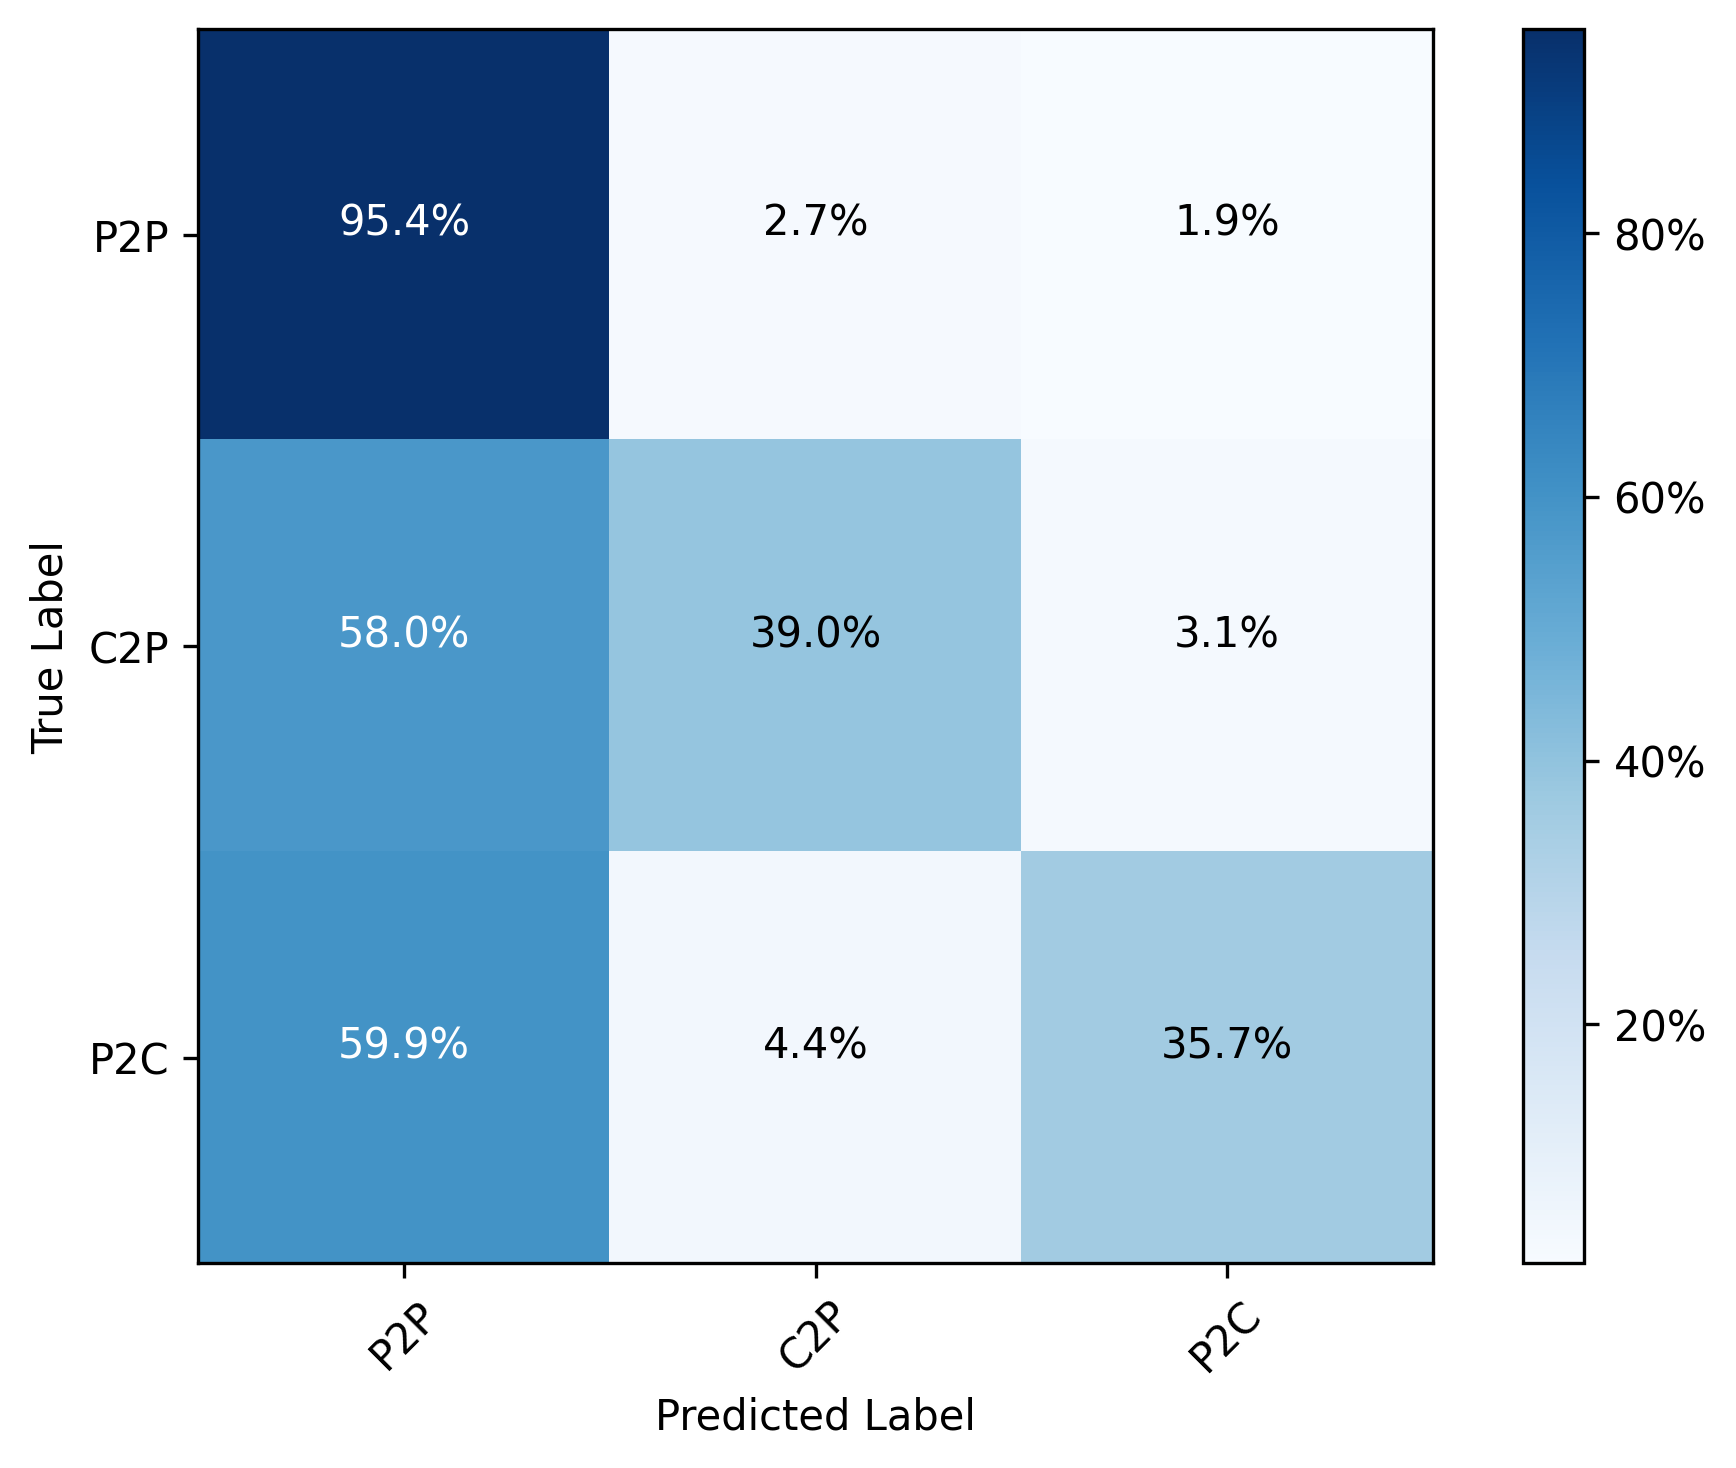
\includegraphics[width=\textwidth]{img/resultados/gnn/partes/caso1_degree/full/Confusion matrix_normalized_febrero_embeddings_ribs_MLP_GraphSAGE_grado_attr_febrero_with_no_batches_with_no_class_weight}
%        \caption{GraphSAGE·MLP - NoBatch-NoW}
%        \label{fig:conf_matrix_gcn_dp}
%    \end{subfigure}
%    \hfill
%    \begin{subfigure}[b]{0.24\textwidth}
%        \centering
%        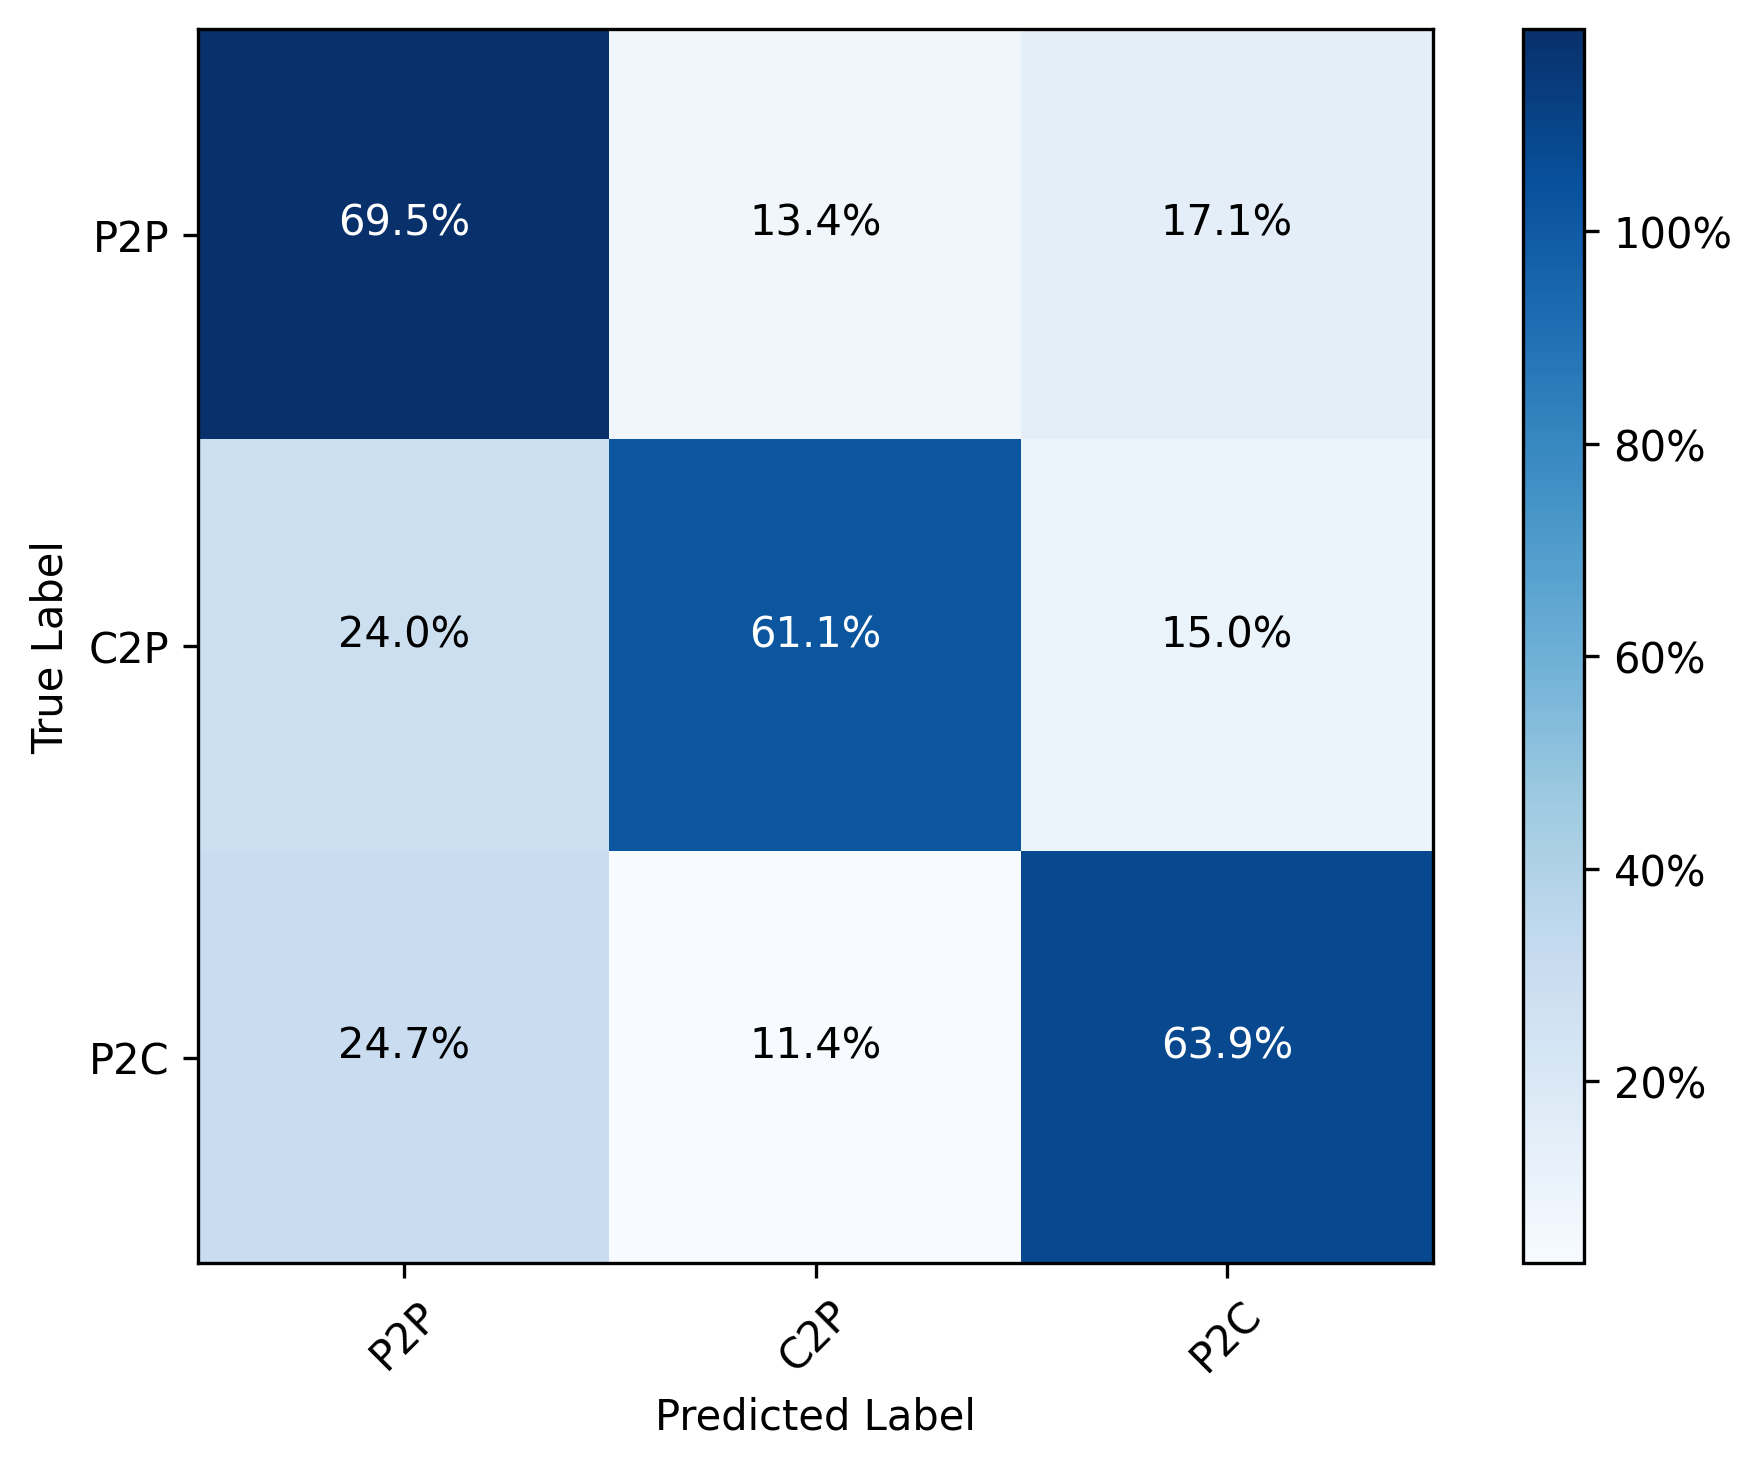
\includegraphics[width=\textwidth]{img/resultados/gnn/partes/caso1_degree/full/Confusion matrix_normalized_febrero_embeddings_ribs_MLP_GraphSAGE_grado_attr_febrero_with_no_batches_with_class_weight}
%        \caption{GraphSAGE·MLP - NoBatch-W}
%        \label{fig:conf_matrix_sage_dp}
%    \end{subfigure}
%    \hfill
%    \begin{subfigure}[b]{0.24\textwidth}
%        \centering
%        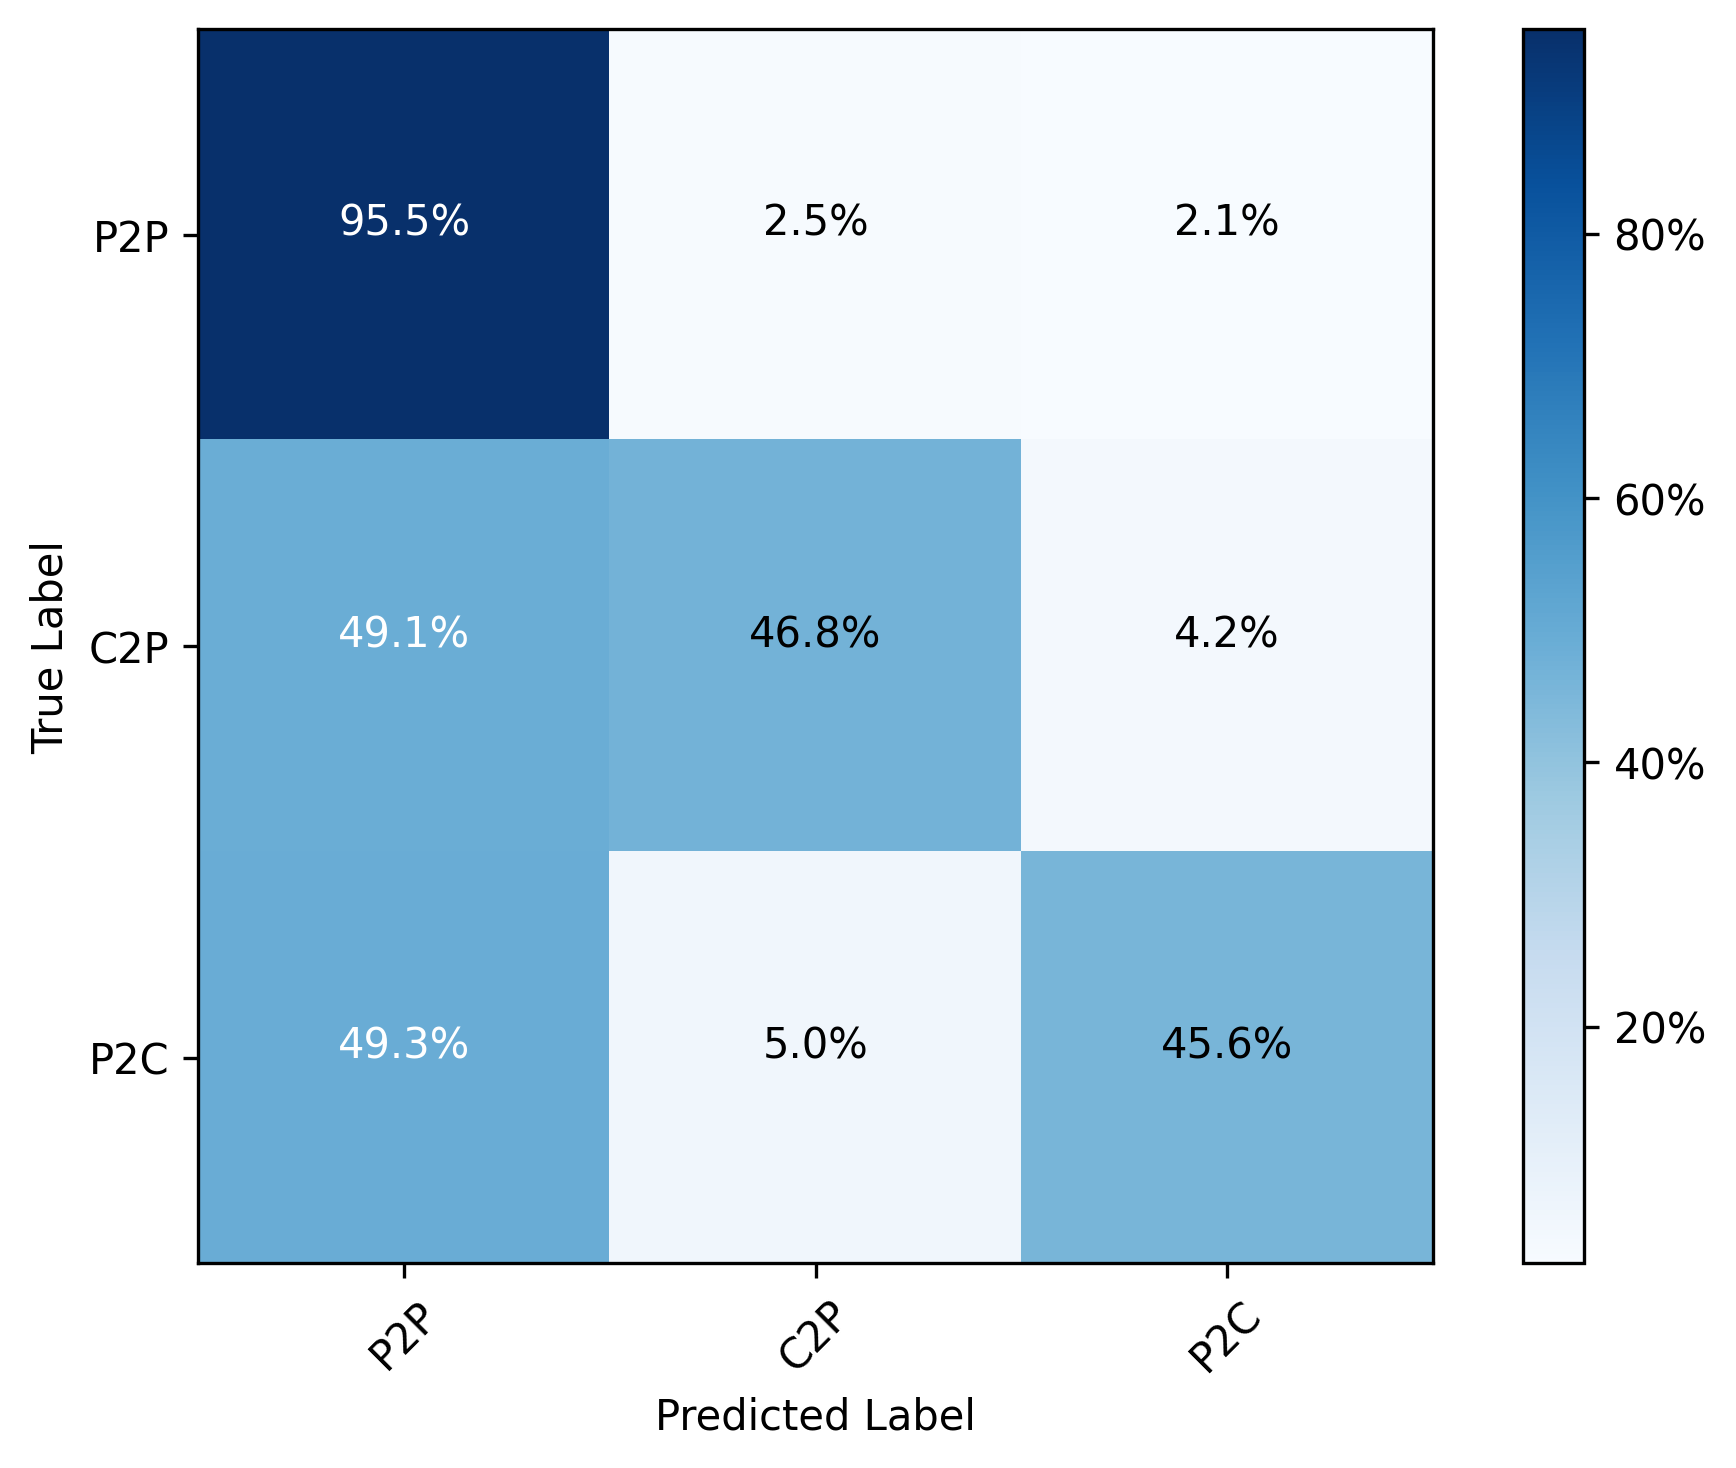
\includegraphics[width=\textwidth]{img/resultados/gnn/partes/caso1_degree/full/Confusion matrix_normalized_febrero_embeddings_ribs_MLP_GraphSAGE_grado_attr_febrero_with_batches_with_no_class_weight}
%        \caption{GraphSAGE·MLP - Batch-NoW }
%        \label{fig:conf_matrix_gat_dp}
%    \end{subfigure}
%    \hfill
%    \begin{subfigure}[b]{0.24\textwidth}
%        \centering
%        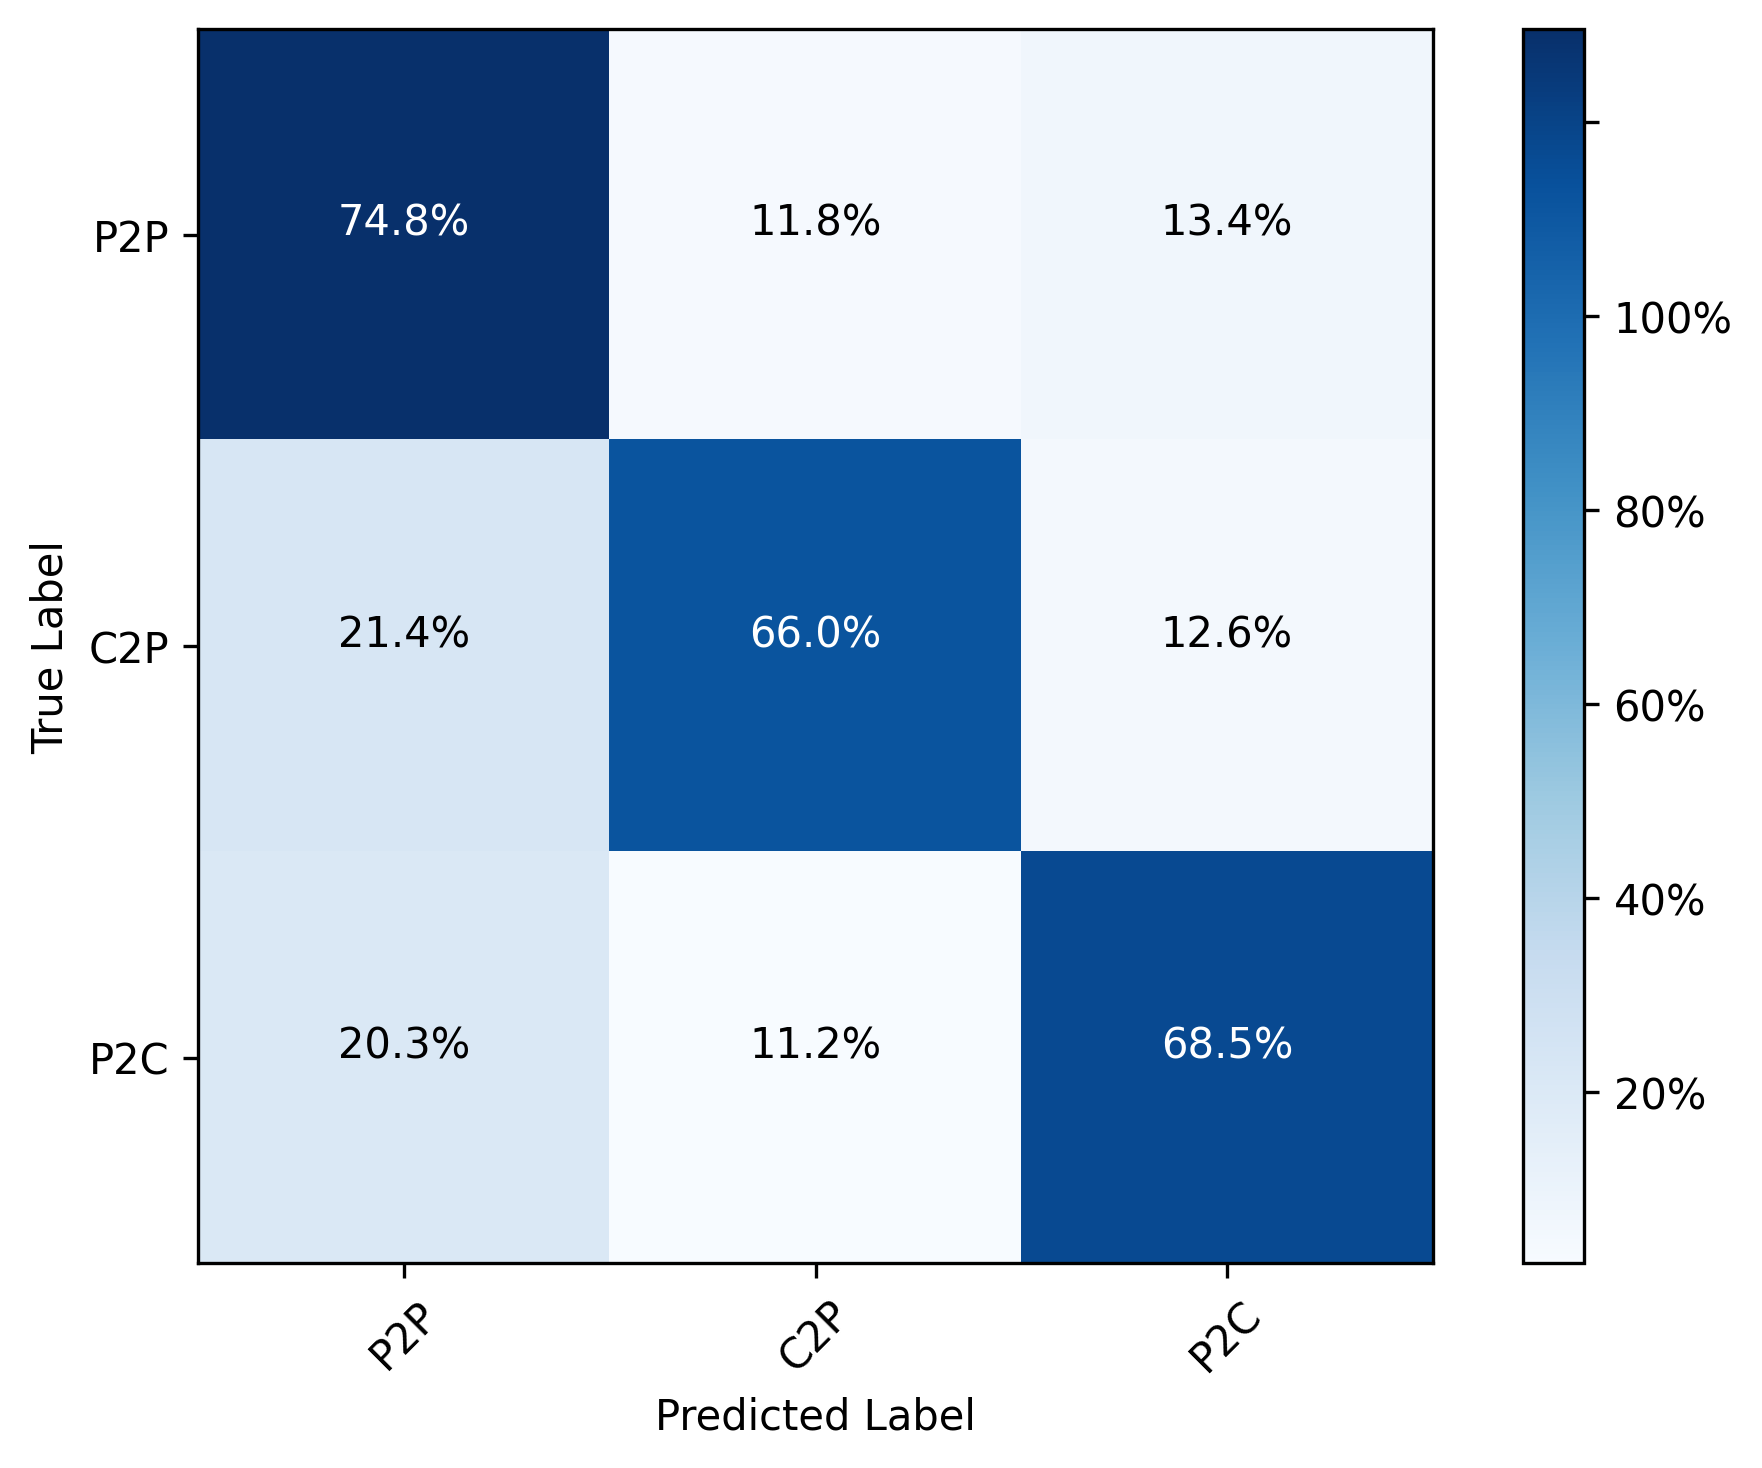
\includegraphics[width=\textwidth]{img/resultados/gnn/partes/caso1_degree/full/Confusion matrix_normalized_febrero_embeddings_ribs_MLP_GraphSAGE_grado_attr_febrero_with_batches_with_class_weight}
%        \caption{GraphSAGE·MLP -> Batch-W }
%        \label{fig:conf_matrix_gat_dp}
%    \end{subfigure}

    %\caption{}
    %\label{fig:...}
%\end{figure}


%\begin{figure}[H]
%    \centering
%    %Sexta Fila: GAT MLP -----------------------------------
%        \begin{subfigure}[b]{0.24\textwidth}
%        \centering
%        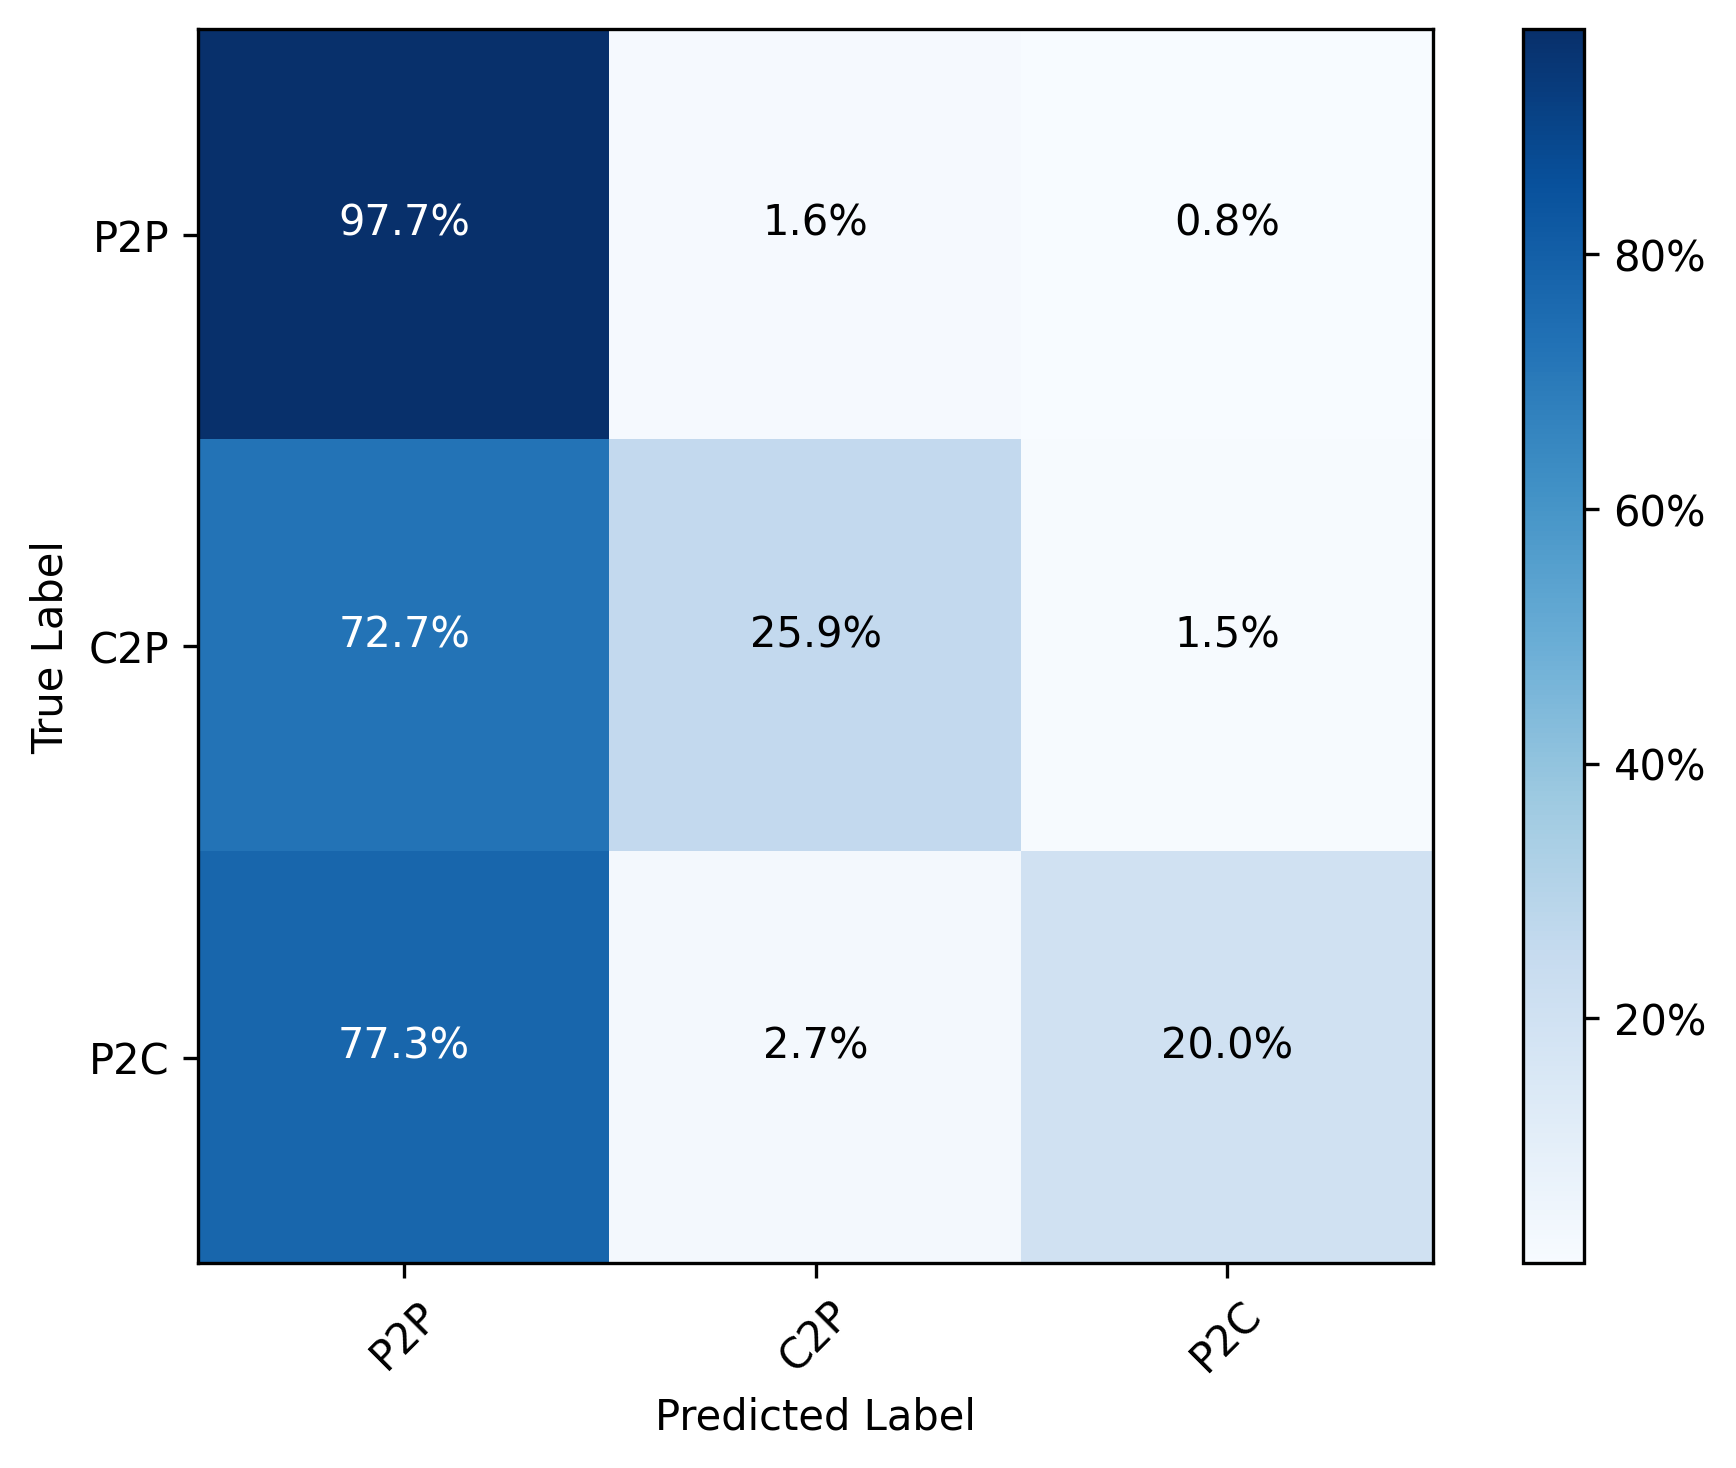
\includegraphics[width=\textwidth]{img/resultados/gnn/partes/caso1_degree/full/Confusion matrix_normalized_febrero_embeddings_ribs_MLP_GAT_grado_attr_febrero_with_no_batches_with_no_class_weight}
%        \caption{GAT·MLP - NoBatch-NoW }
%        \label{fig:conf_matrix_gcn_dp}
%    \end{subfigure}
%    \hfill
%    \begin{subfigure}[b]{0.24\textwidth}
%        \centering
%        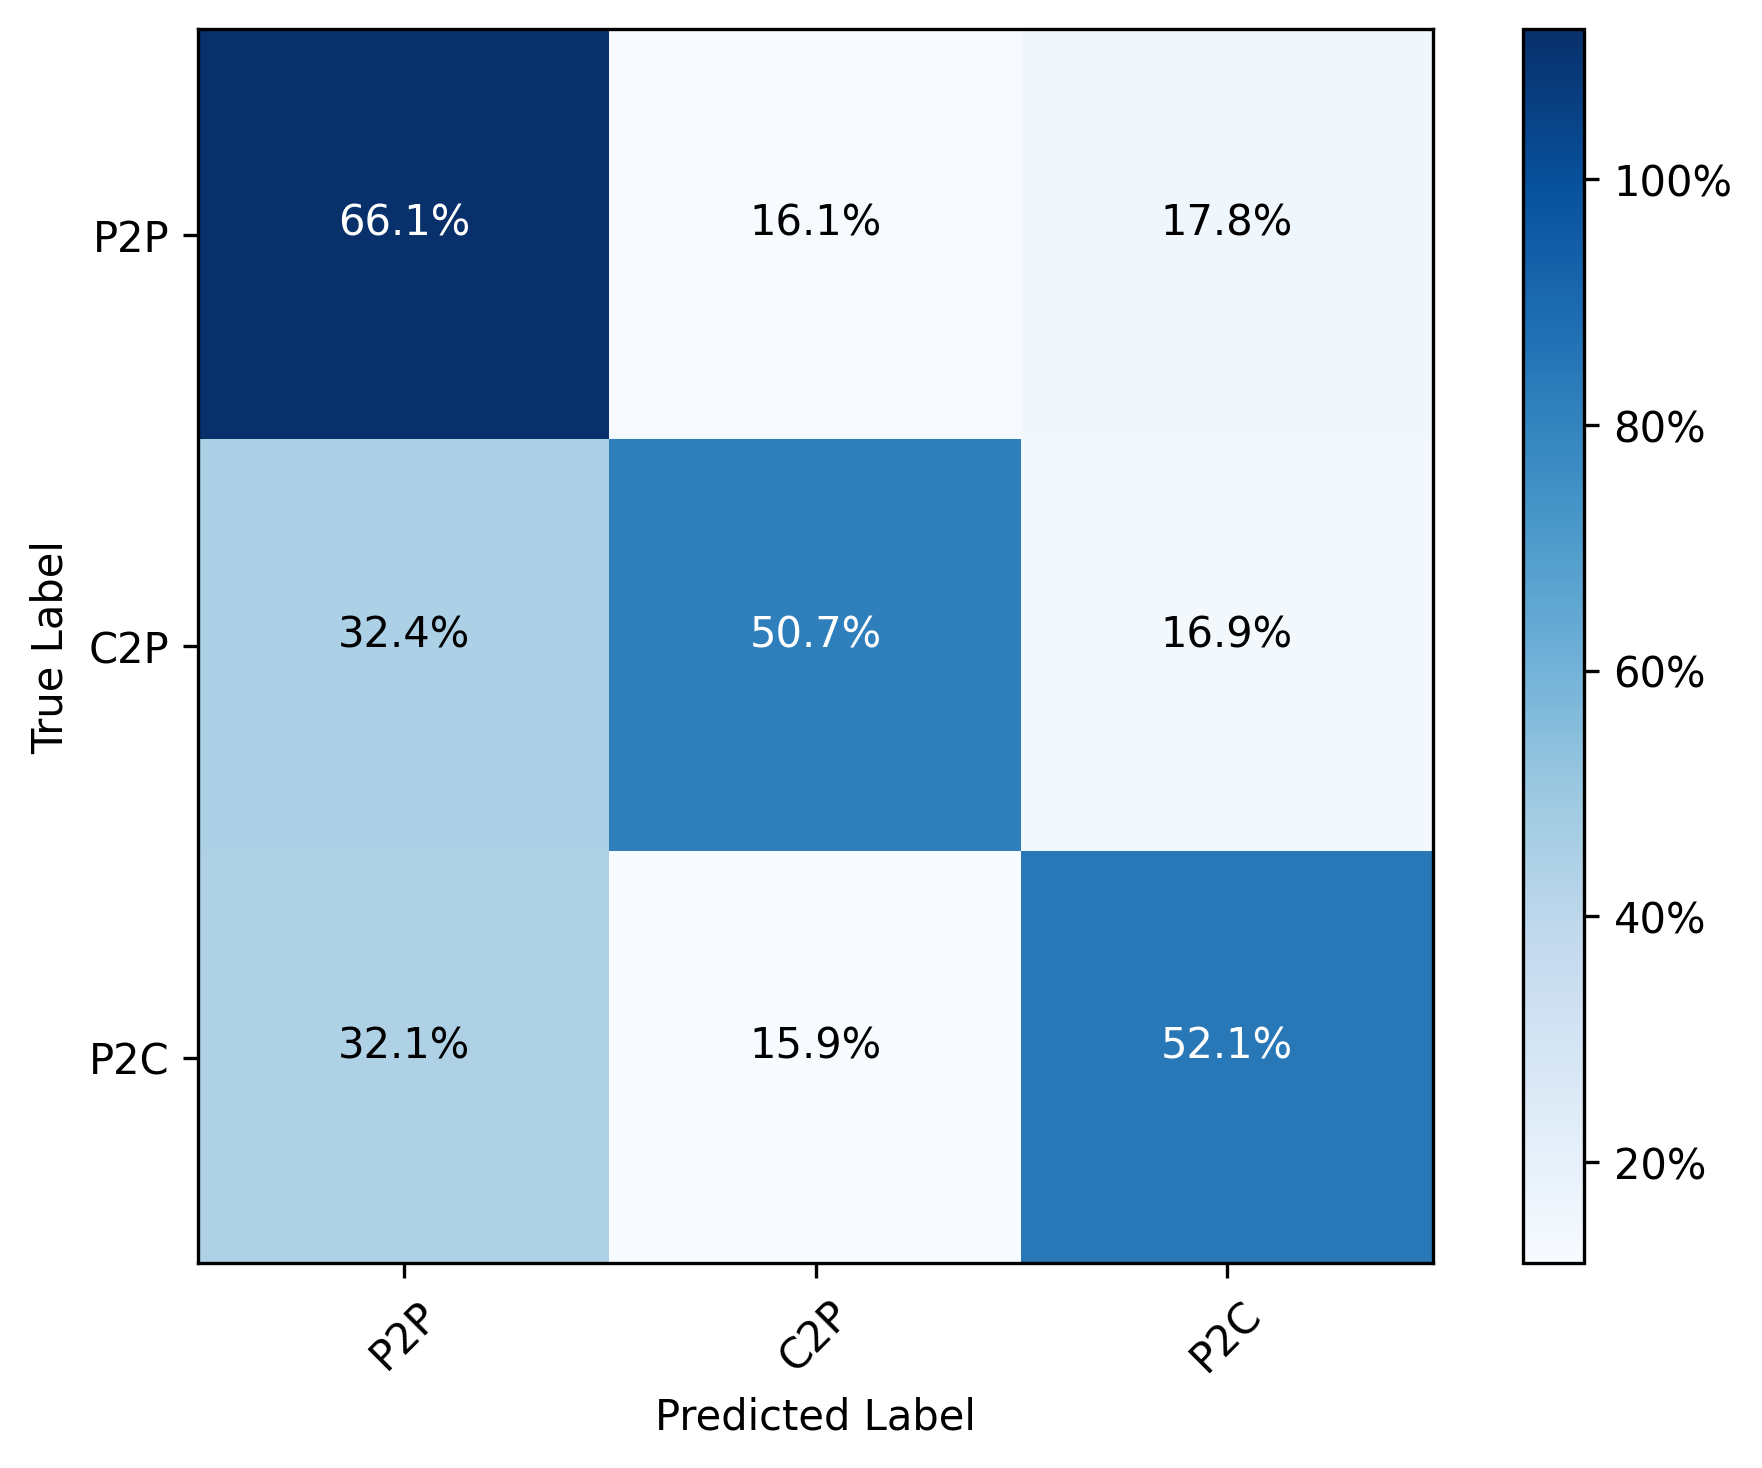
\includegraphics[width=\textwidth]{img/resultados/gnn/partes/caso1_degree/full/Confusion matrix_normalized_febrero_embeddings_ribs_MLP_GAT_grado_attr_febrero_with_no_batches_with_class_weight}
%        \caption{GAT·MLP - NoBatch-W}
%        \label{fig:conf_matrix_sage_dp}
%    \end{subfigure}
%    \hfill
%    \begin{subfigure}[b]{0.24\textwidth}
%        \centering
%        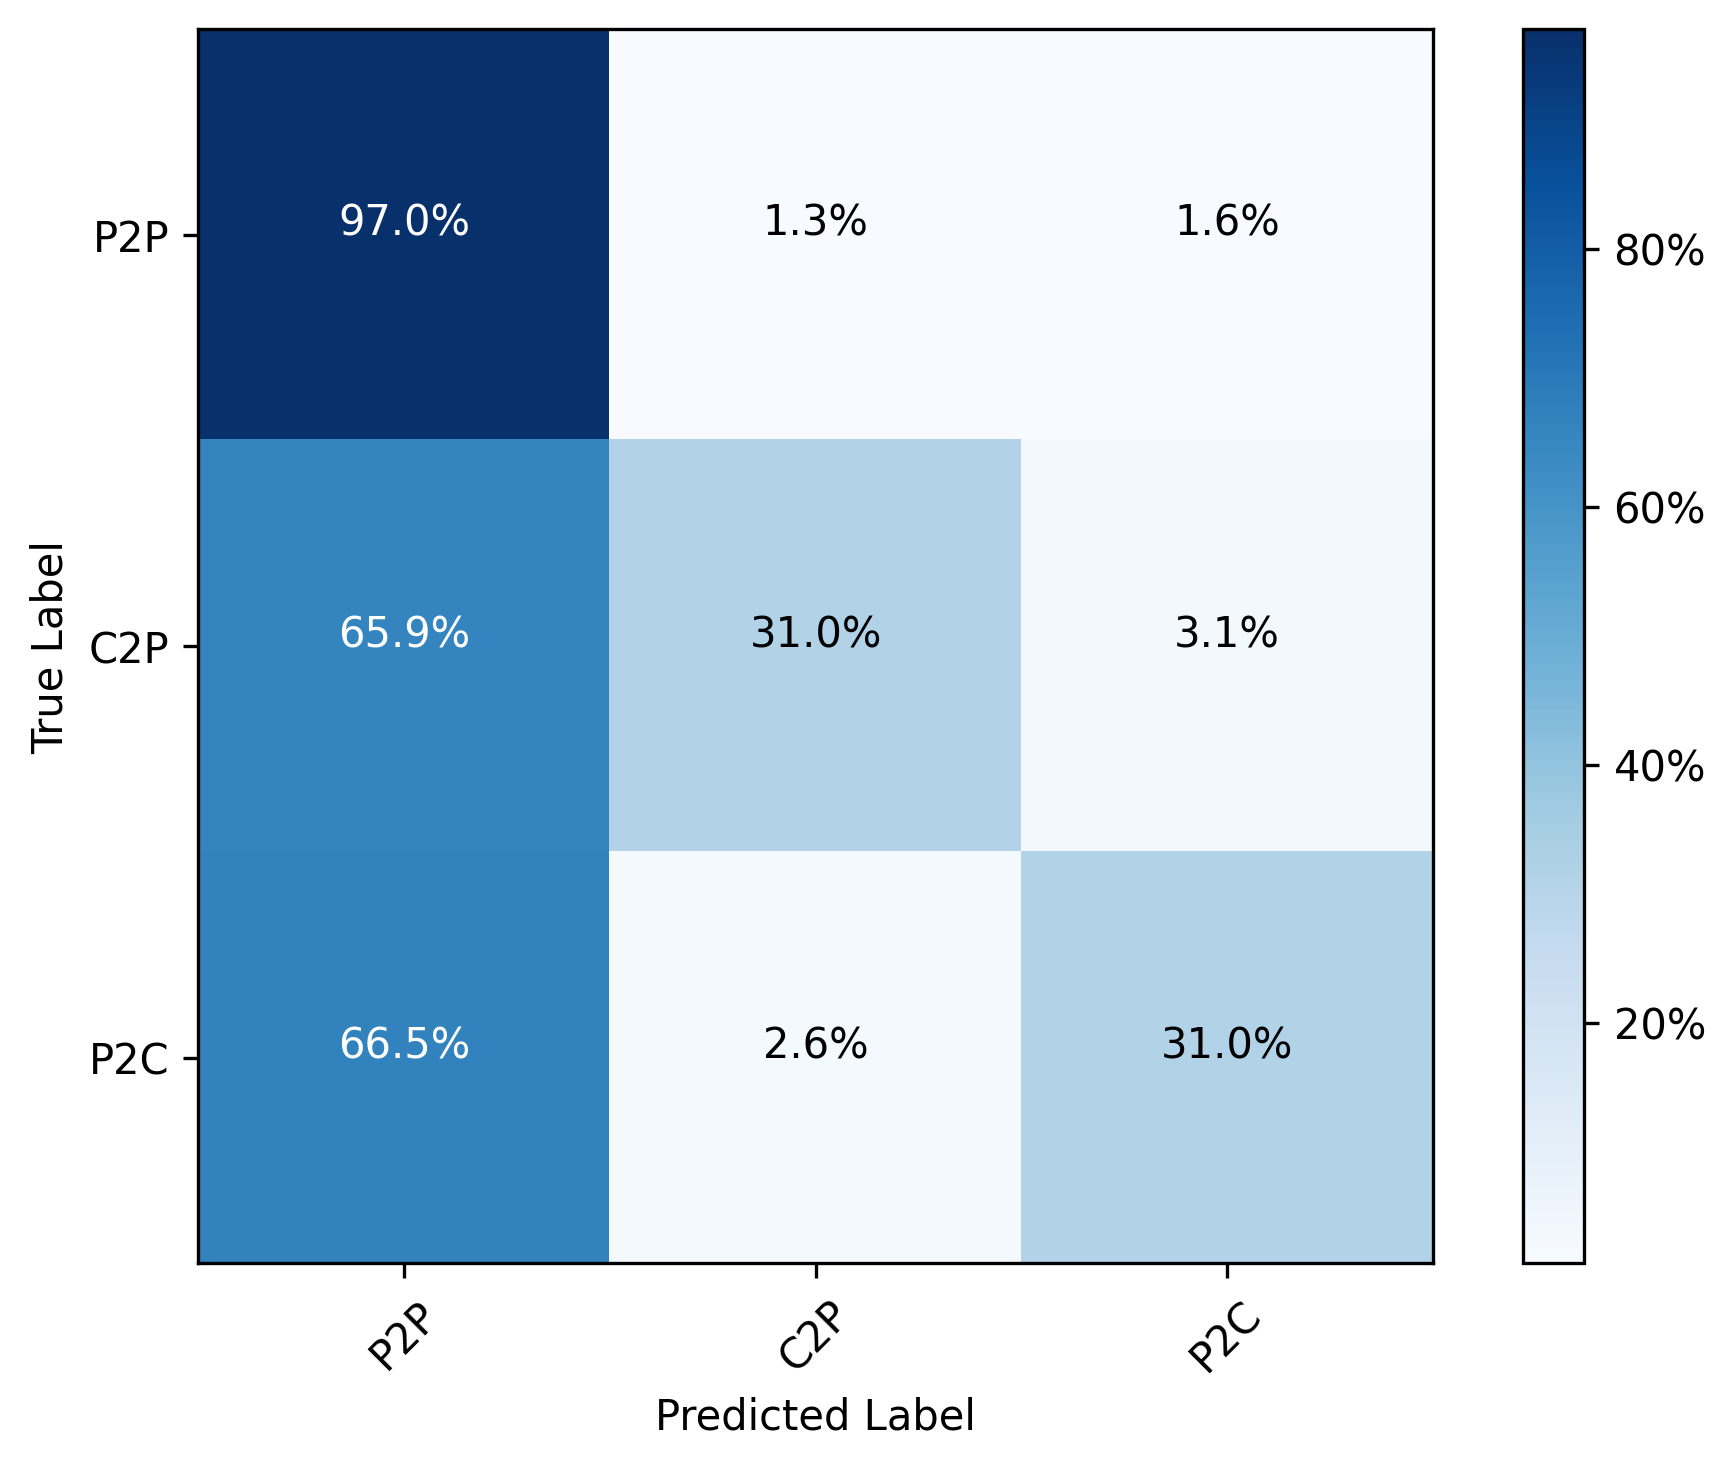
\includegraphics[width=\textwidth]{img/resultados/gnn/partes/caso1_degree/full/Confusion matrix_normalized_febrero_embeddings_ribs_MLP_GAT_grado_attr_febrero_with_batches_with_no_class_weight}
%        \caption{GAT·MLP - Batch-NoW }
%        \label{fig:conf_matrix_gat_dp}
%    \end{subfigure}
%    \hfill
%    \begin{subfigure}[b]{0.24\textwidth}
%        \centering
%        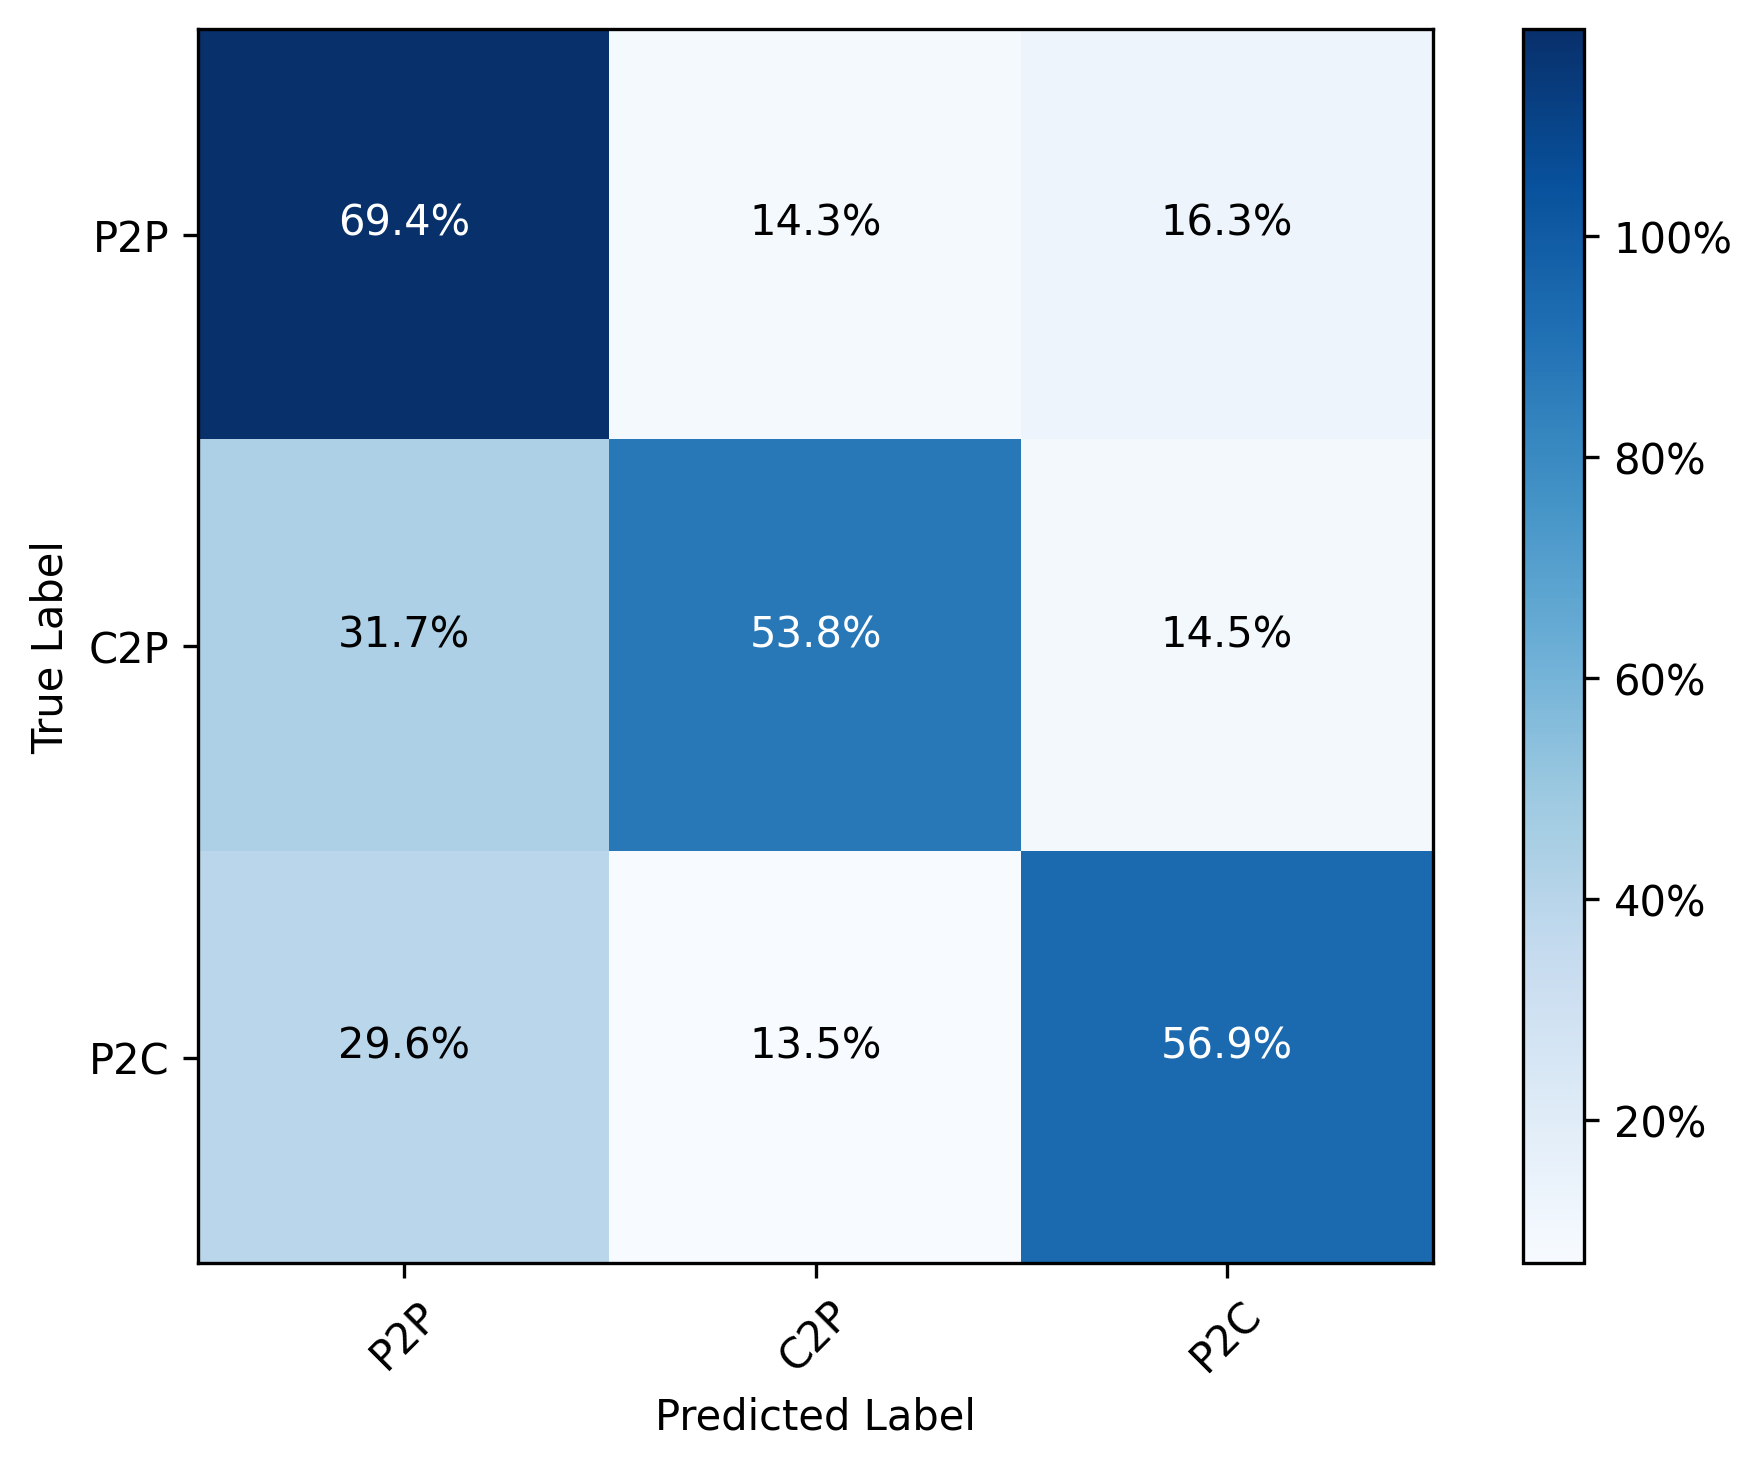
\includegraphics[width=\textwidth]{img/resultados/gnn/partes/caso1_degree/full/Confusion matrix_normalized_febrero_embeddings_ribs_MLP_GAT_grado_attr_febrero_with_batches_with_class_weight}
%        \caption{GAT·MLP - Batch-W }
%        \label{fig:conf_matrix_gat_dp}
%    \end{subfigure}
    
 %   \caption{Matrices de confusión normalizadas para las 24 combinaciones evaluadas: tres codificadores (GCN, GraphSAGE, GAT) × dos decodificadores (Dot Product, MLP) × cuatro configuraciones de entrenamiento.  
%Las configuraciones se identifican como \textbf{NoBatch-NoW} (sin mini-batching ni pesos de clase), \textbf{NoBatch-W} (sin mini-batching con pesos de clase), \textbf{Batch-NoW} (con mini-batching sin pesos de clase) y \textbf{Batch-W} (con mini-batching y pesos de clase).}
%    \label{fig:anex:matrices_confusion_experimentos_gnns_decoder}
%\end{figure}


%////////////////////////////////////////////////////////////////
%\subsubsection{Caso 2: Atributos obtenidos desde PeeringDB con predicción de enlaces} \label{sec:anexo_por_partes_caso_2}



















%\subsubsubsection{Análisis con restricción de 1.000.000 AS\_PATHS}




%Resultados obtenidos al generar los embeddings a partir de 1.000.000 de rutas AS\_PATH. Tabla \ref{tab:accuracy_gnn_1millon_caso2} presenta los valores de AUC y accuracy obtenidos por cada combinación de encoder y decoder. Figura \ref{fig:partes_caso_2_comparacion_roc_auc_anexo_1millon} complementa esta información mostrando las curvas ROC y la distribución de los casos positivos y negativos. Finalmente Figura~\ref{fig:matrices_confusion_partes_caso2_1millon} presenta matrices de confusión para los diferentes arquitecturas que se utilizo para crear las representaciones vectoriales de los Sistemas Autónomos.\\


%\begin{figure}[H]
%    \centering
    % Primera fila
%    \begin{subfigure}[b]{0.45\textwidth}
%        \centering
%        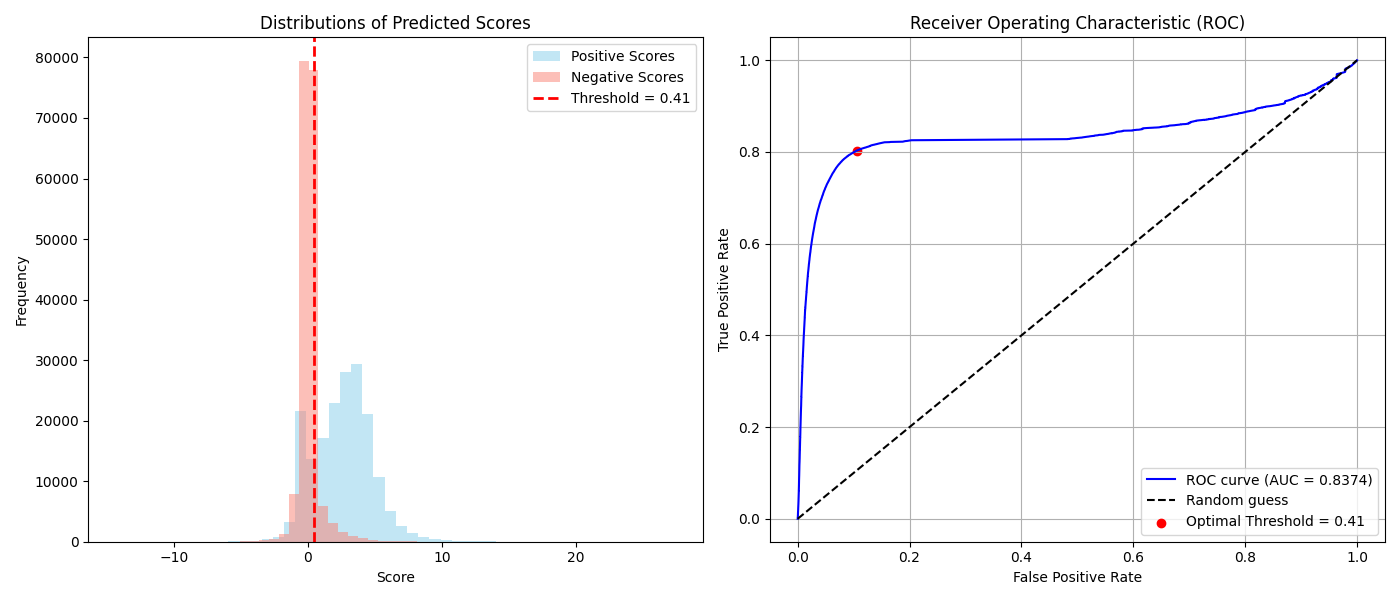
\includegraphics[width=\textwidth]{img/resultados/gnn/partes/caso2_mis_attr/anexo/curva_roc/mis_attr/roc_curve_GCN_DotProduct.png}
%        \caption{GCN + Dot Product}
%        \label{fig:conf_matrix_gcn_dp}
%    \end{subfigure}
%    \hfill
%    \begin{subfigure}[b]{0.45\textwidth}
%        \centering
%        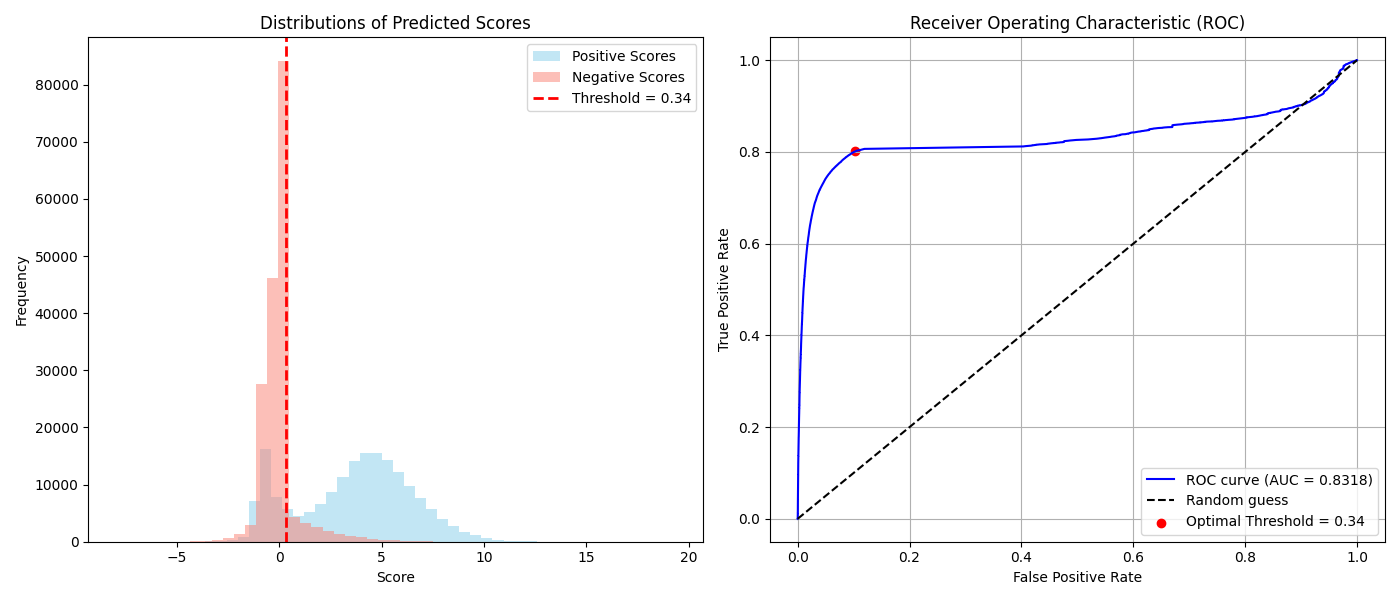
\includegraphics[width=\textwidth]{img/resultados/gnn/partes/caso2_mis_attr/anexo/curva_roc/mis_attr/roc_curve_GraphSAGE_DotProduct.png}
%        \caption{GraphSAGE + Dot Product}
%        \label{fig:conf_matrix_sage_dp}
%    \end{subfigure}

%    \vspace{0.5cm}

    % Segunda fila
%    \begin{subfigure}[b]{0.45\textwidth}
%        \centering
%        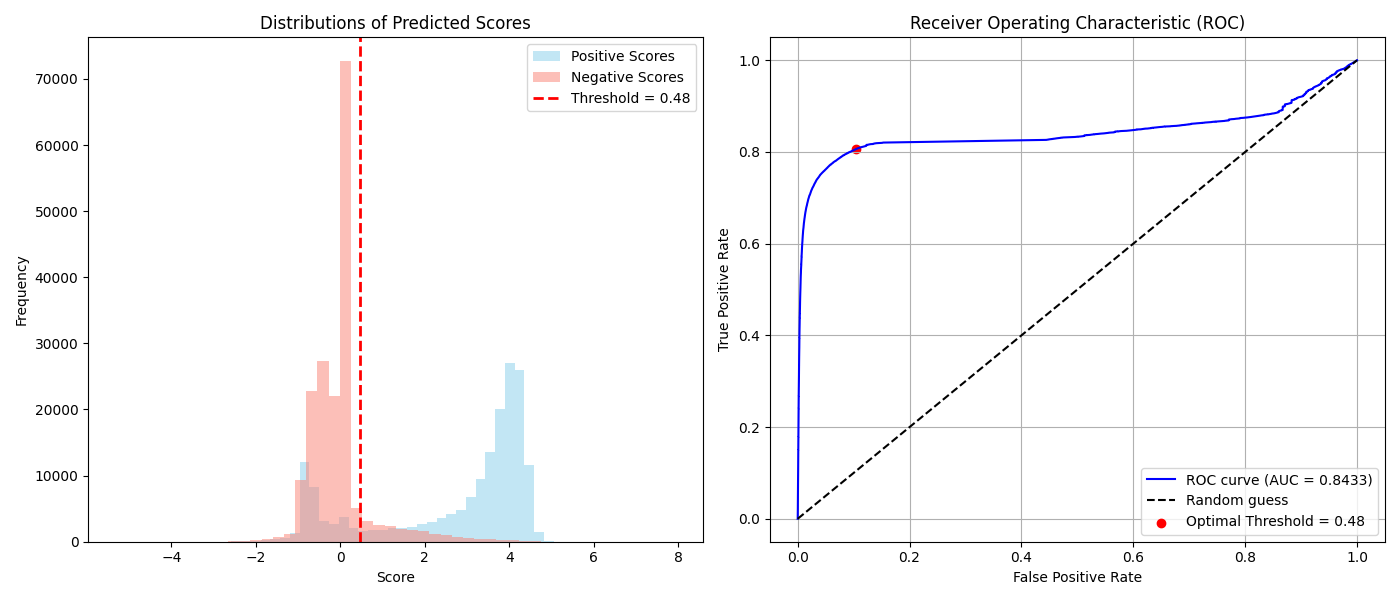
\includegraphics[width=\textwidth]{img/resultados/gnn/partes/caso2_mis_attr/anexo/curva_roc/mis_attr/roc_curve_GAT_DotProduct.png}
%        \caption{GAT + Dot Product}
%        \label{fig:conf_matrix_gat_dp}
%    \end{subfigure}
%    \hfill
%    \begin{subfigure}[b]{0.45\textwidth}
%        \centering
%        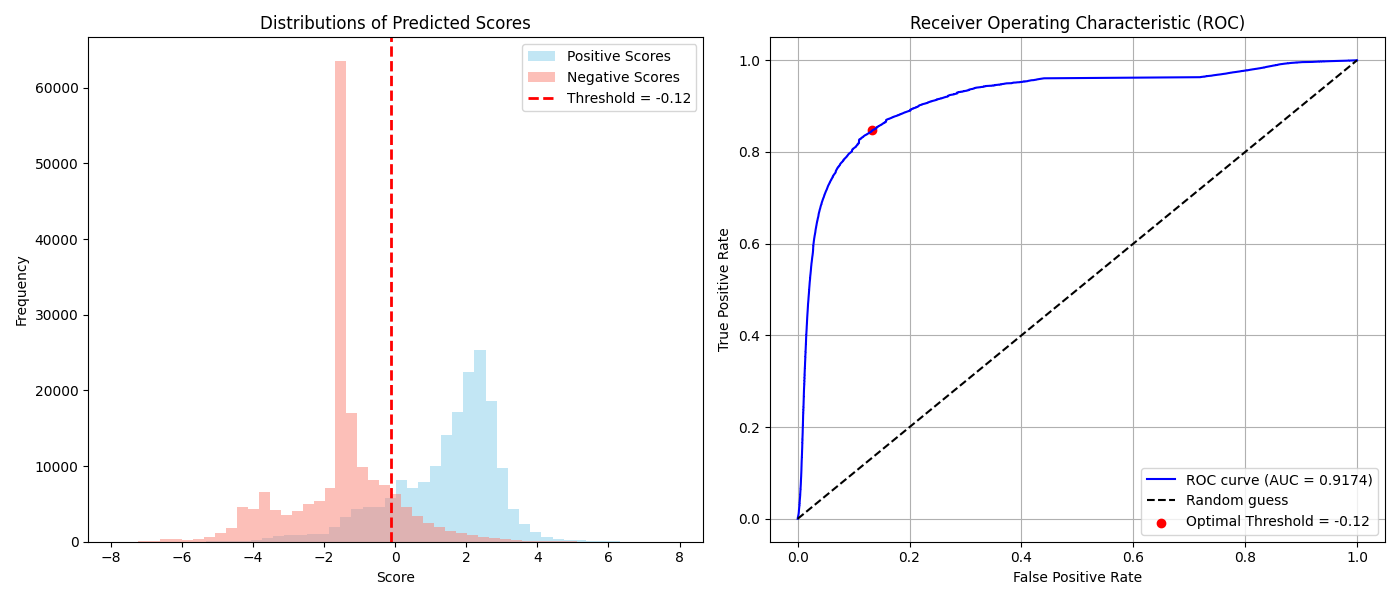
\includegraphics[width=\textwidth]{img/resultados/gnn/partes/caso2_mis_attr/anexo/curva_roc/mis_attr/roc_curve_GCN_MLP.png}
%        \caption{GCN + MLP}
%        \label{fig:conf_matrix_gcn_mlp}
%    \end{subfigure}

%    \vspace{0.5cm}

    % Tercera fila
%    \begin{subfigure}[b]{0.45\textwidth}
%        \centering
%        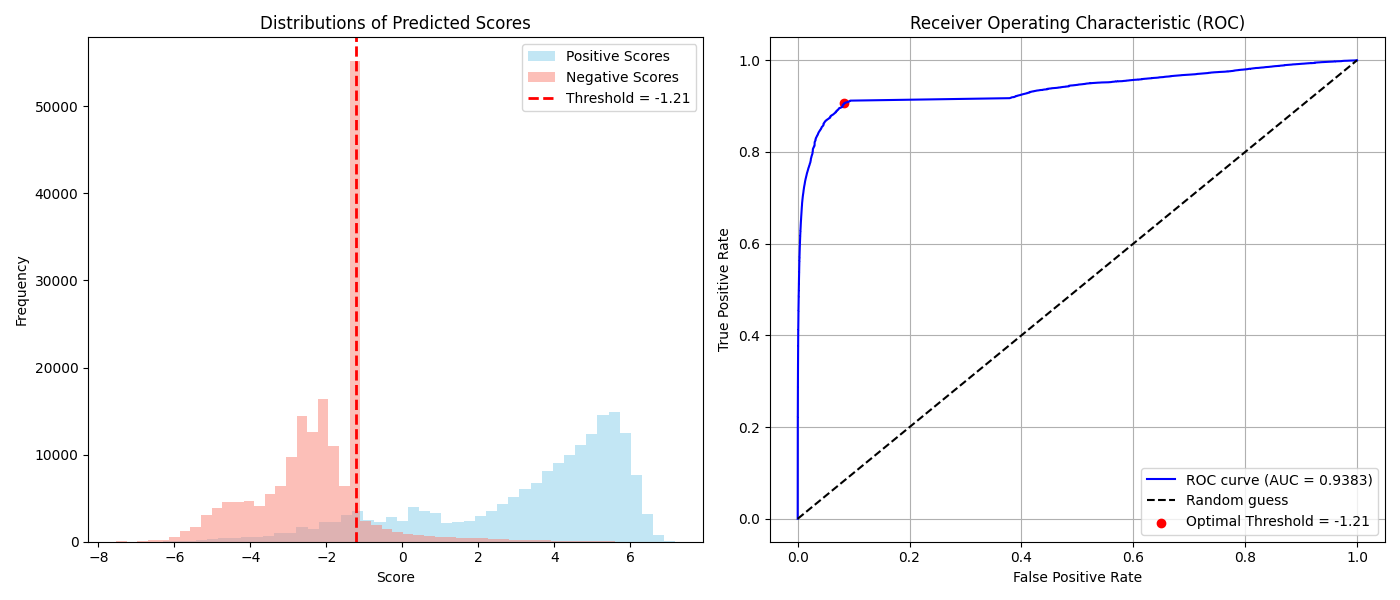
\includegraphics[width=\textwidth]{img/resultados/gnn/partes/caso2_mis_attr/anexo/curva_roc/mis_attr/roc_curve_GraphSAGE_MLP.png}
%        \caption{GraphSAGE + MLP}
%        \label{fig:conf_matrix_sage_mlp}
%    \end{subfigure}
%    \hfill
%    \begin{subfigure}[b]{0.45\textwidth}
%        \centering
%        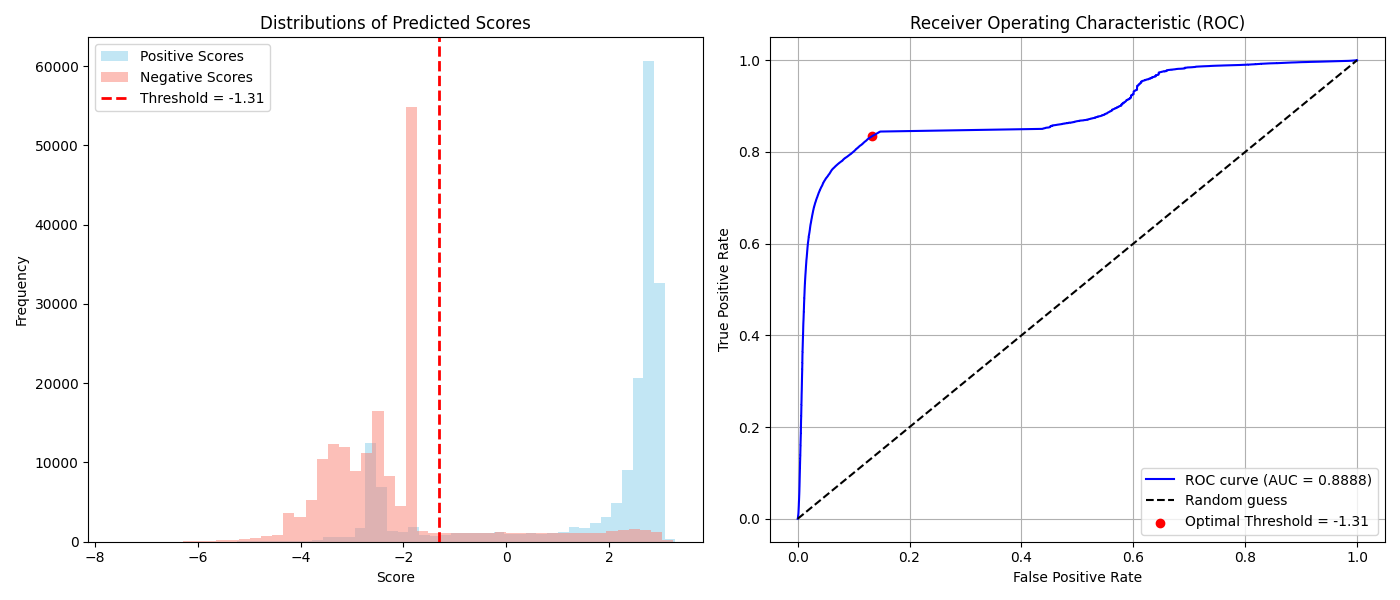
\includegraphics[width=\textwidth]{img/resultados/gnn/partes/caso2_mis_attr/anexo/curva_roc/mis_attr/roc_curve_GAT_MLP.png}
%        \caption{GAT + MLP}
%        \label{fig:conf_matrix_gat_mlp}
%    \end{subfigure}
%    \caption{Curvas ROC y distribución de resultados con el mejor umbral.}
% \label{fig:partes_caso_2_comparacion_roc_auc_anexo_1millon}
%\end{figure}

%\begin{table}[ht]
%    \centering
%    \begin{tabular}{lccccc}
%    \hline
%    \textbf{Método} & \textbf{AUC} & \textbf{Accuracy inferencia }  \\
%    \hline
%    GCN + producto punto &  0.865 & 70.15\% \\
%    GraphSAGE + producto punto & 0.811 &  67.81\% \\
%    GAT + producto punto & 0.826 & 70.32\% \\
%    GCN + MLP  & 0.963 & 70.78\% \\
%    GraphSAGE + MLP  & 0.869 & 69.74\% \\
%    GAT + MLP &  856 & 69.20\% \\
%    \hline
%    \end{tabular}
%    \label{tab:comparacion_accuracy_caso2}
%    \caption{Accuracy de la inferencia con link prediction para la creacion de embeddings.}
%\end{table}
% \begin{figure}[H]
%     \centering
%     % Primera fila
%     \begin{subfigure}[b]{0.3\textwidth}
%         \centering
%         \includegraphics[width=\textwidth]{img/resultados/gnn/partes/caso2_mis_attr/anexo/matriz_confusion/confusion matrix_febrero_embeddings_ribs_DP_GCN.png}
%         \caption{GCN + Dot Product}
%         \label{fig:conf_matrix_gcn_dp}
%     \end{subfigure}
%     \hfill
%     \begin{subfigure}[b]{0.3\textwidth}
%         \centering
%         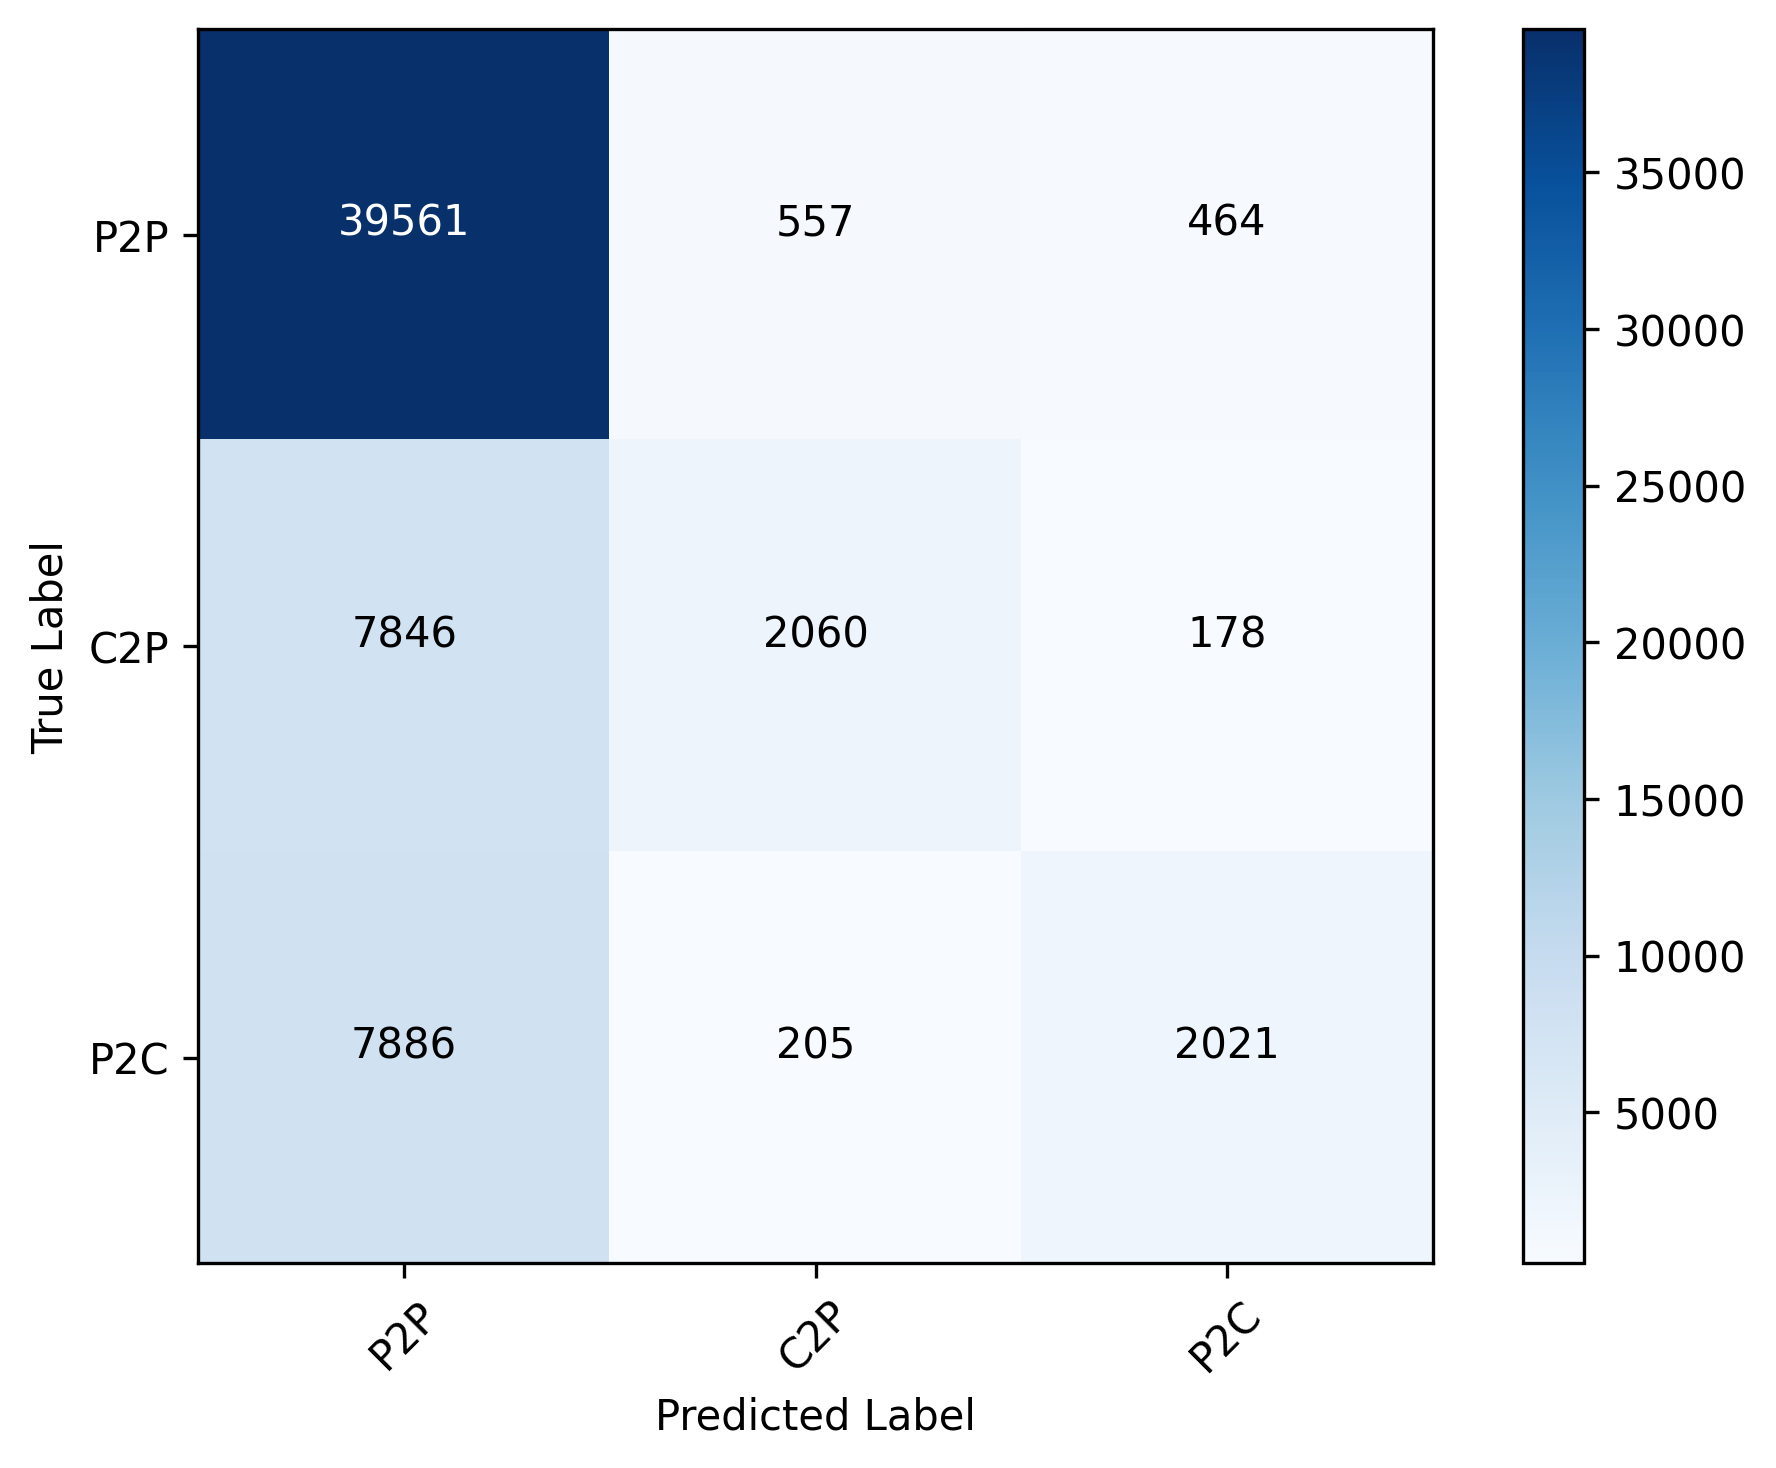
\includegraphics[width=\textwidth]{img/resultados/gnn/partes/caso2_mis_attr/anexo/matriz_confusion/Confusion matrix_febrero_embeddings_ribs_DP_GraphSAGE.png}
%         \caption{GraphSAGE + Dot Product}
%         \label{fig:conf_matrix_sage_dp}
%     \end{subfigure}
%     \hfill
%     \begin{subfigure}[b]{0.3\textwidth}
%         \centering
%         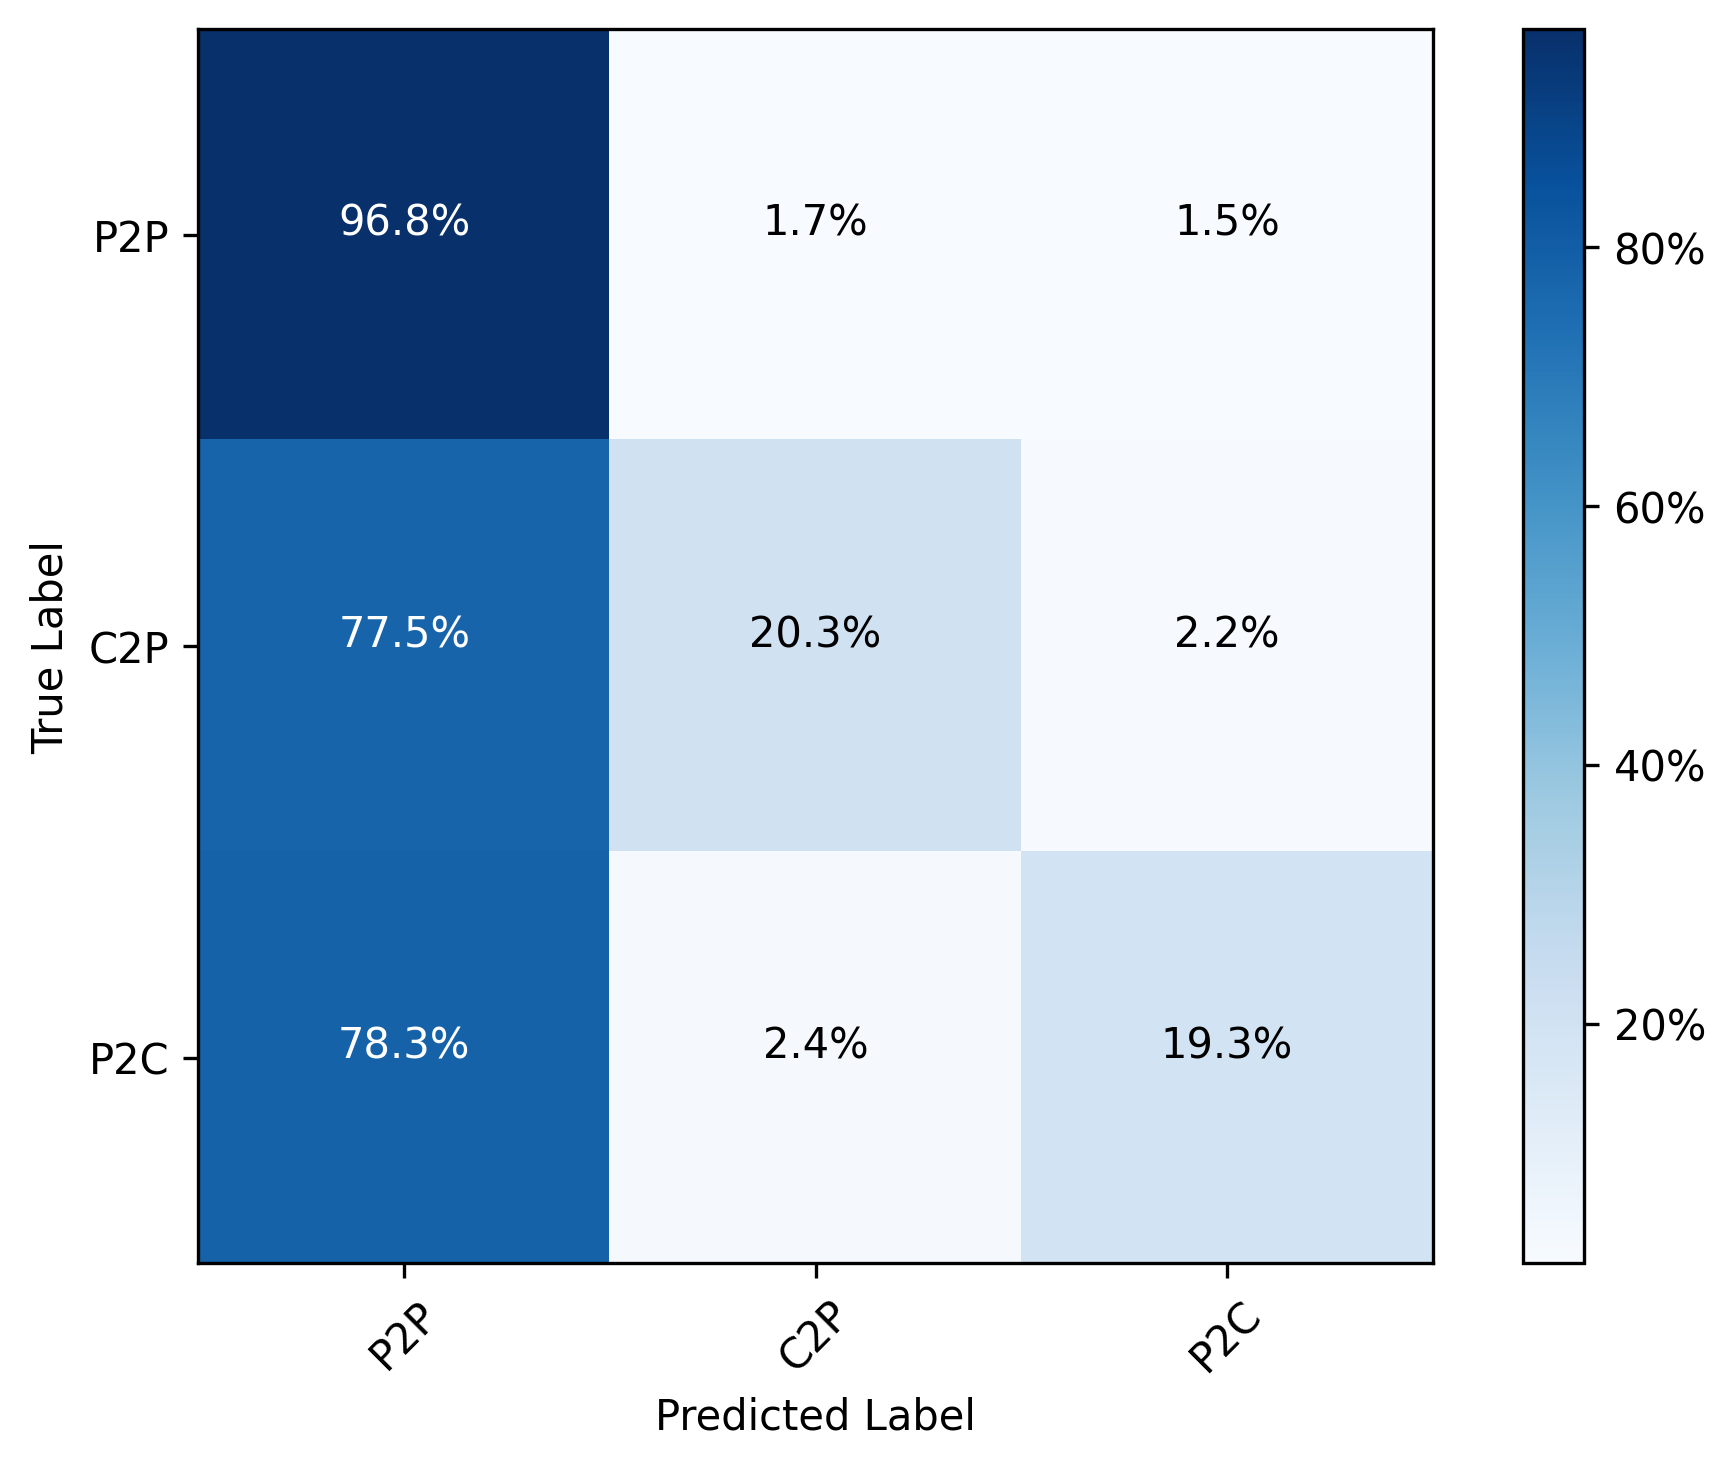
\includegraphics[width=\textwidth]{img/resultados/gnn/partes/caso2_mis_attr/anexo/matriz_confusion/Confusion matrix_normalized_febrero_embeddings_ribs_DP_GAT.png}
%         \caption{GAT + Dot Product}
%         \label{fig:conf_matrix_gat_dp}
%     \end{subfigure}
    
%     \vspace{0.5cm}
%     % Segunda fila
%     \begin{subfigure}[b]{0.3\textwidth}
%         \centering
%         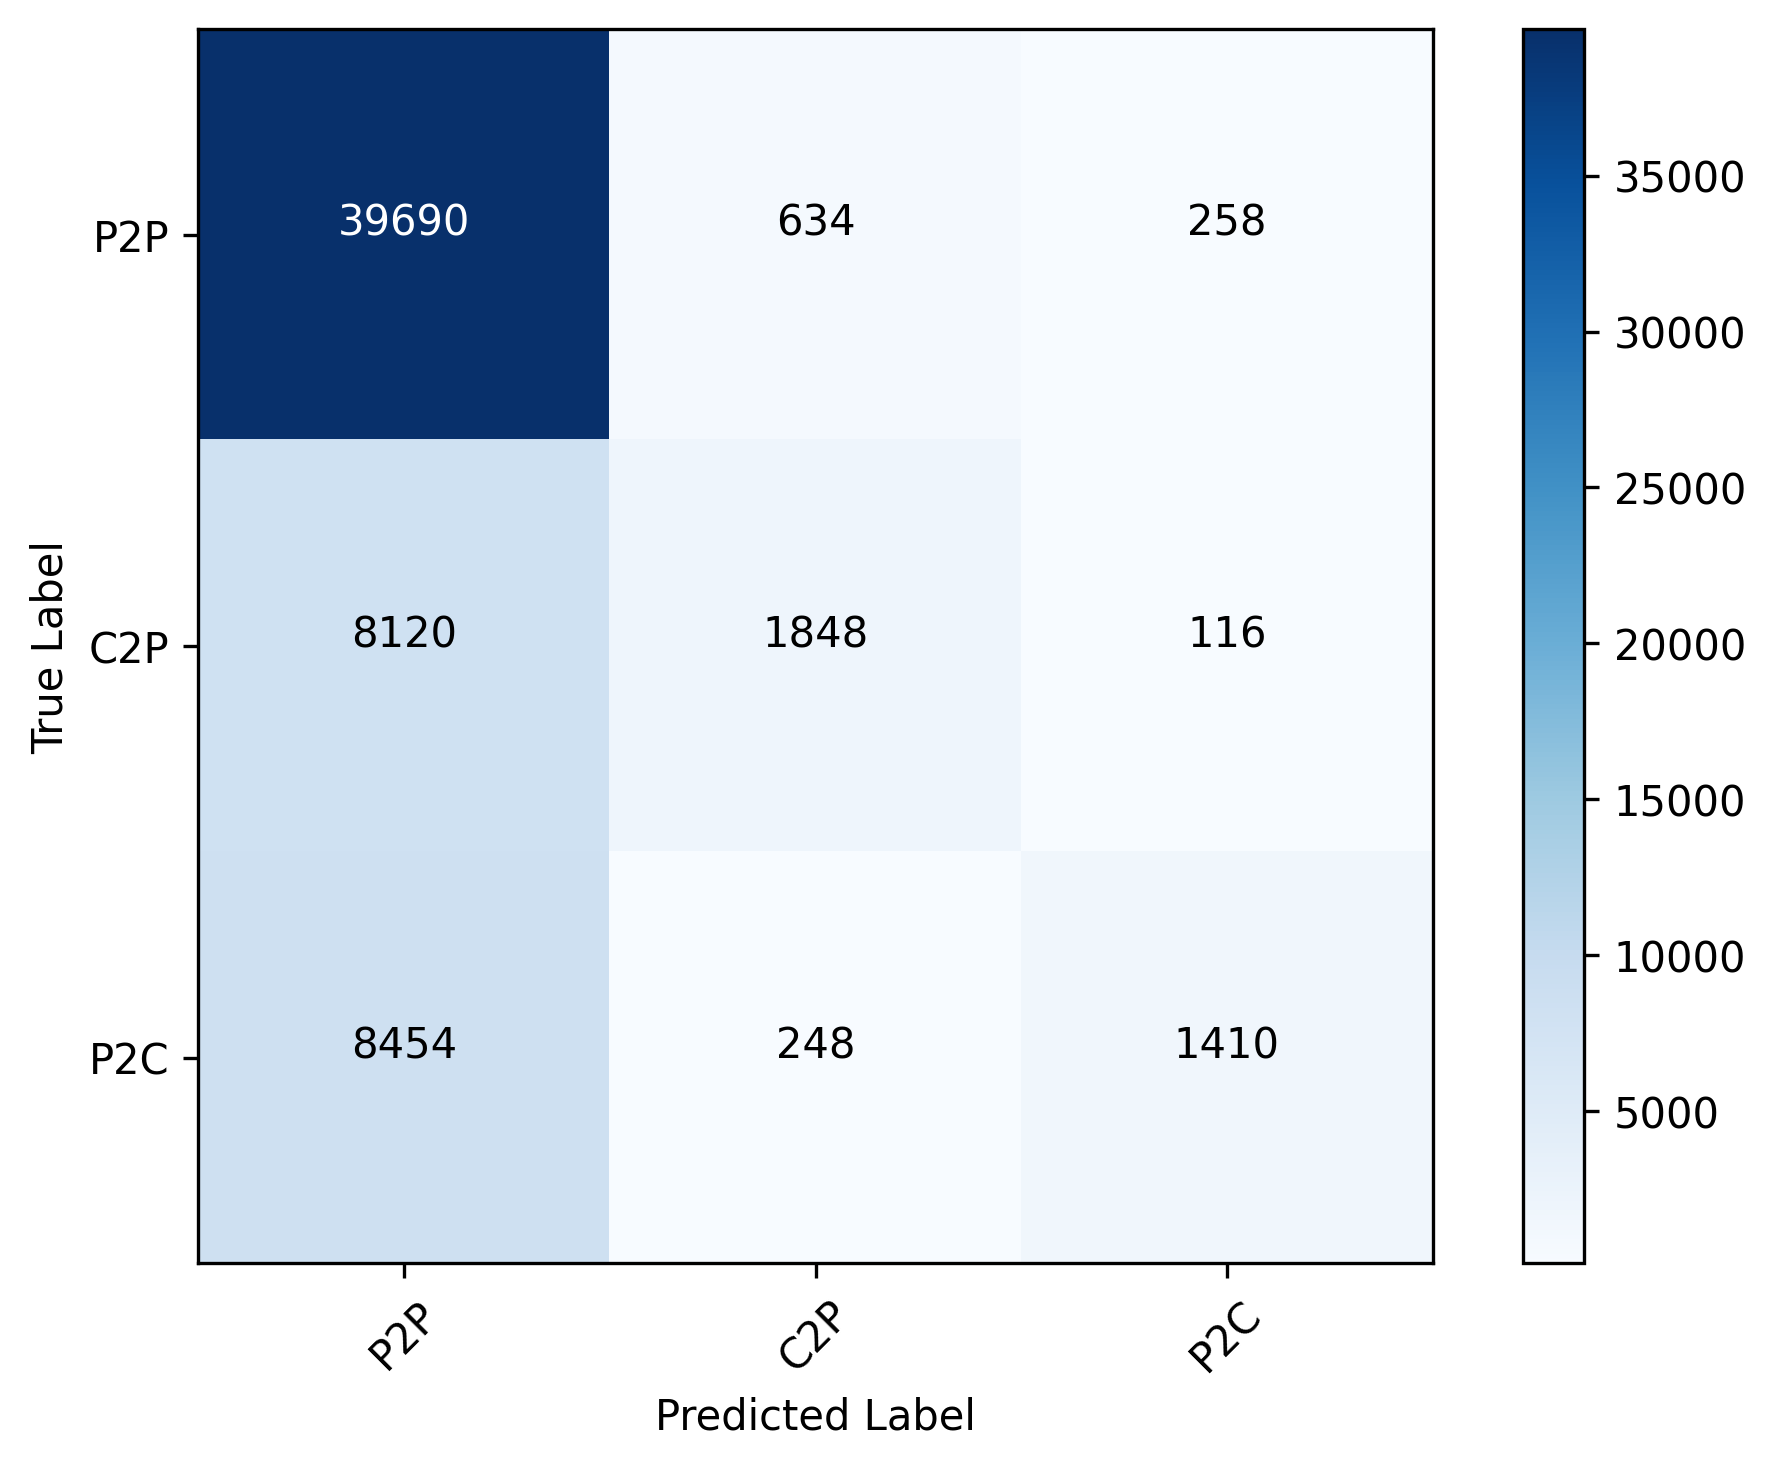
\includegraphics[width=\textwidth]{img/resultados/gnn/partes/caso2_mis_attr/anexo/matriz_confusion/Confusion matrix_febrero_embeddings_ribs_MLP_GCN.png}
%         \caption{GCN + MLP}
%         \label{fig:conf_matrix_gcn_mlp}
%     \end{subfigure}
%     \hfill
%     \begin{subfigure}[b]{0.3\textwidth}
%         \centering
%         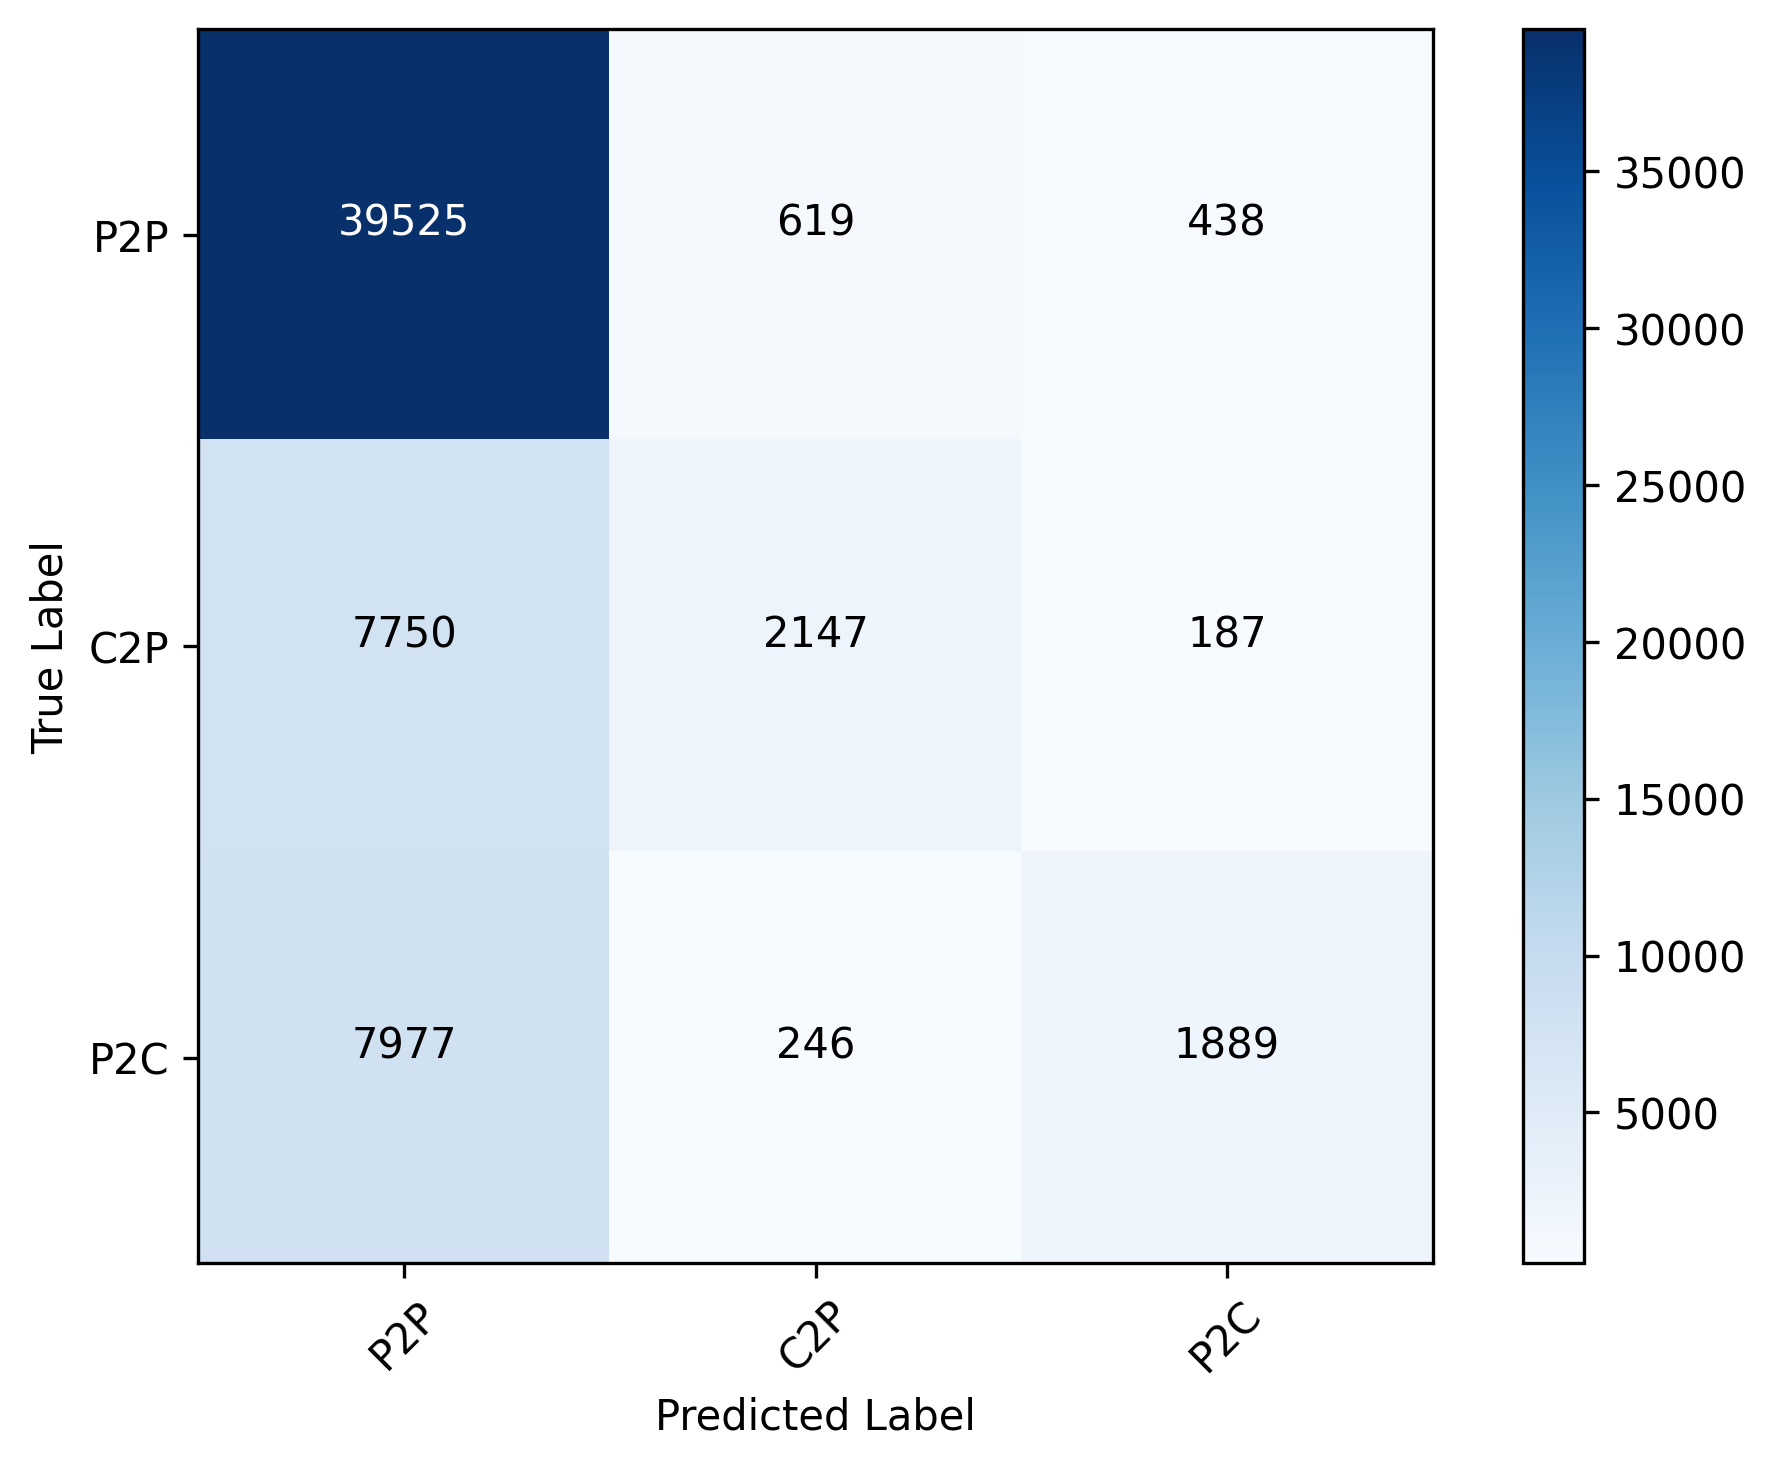
\includegraphics[width=\textwidth]{img/resultados/gnn/partes/caso2_mis_attr/anexo/matriz_confusion/Confusion matrix_febrero_embeddings_ribs_MLP_GraphSAGE.png}
%         \caption{GraphSAGE + MLP}
%         \label{fig:conf_matrix_sage_mlp}
%     \end{subfigure}
%     \hfill
%     \begin{subfigure}[b]{0.3\textwidth}
%         \centering
%         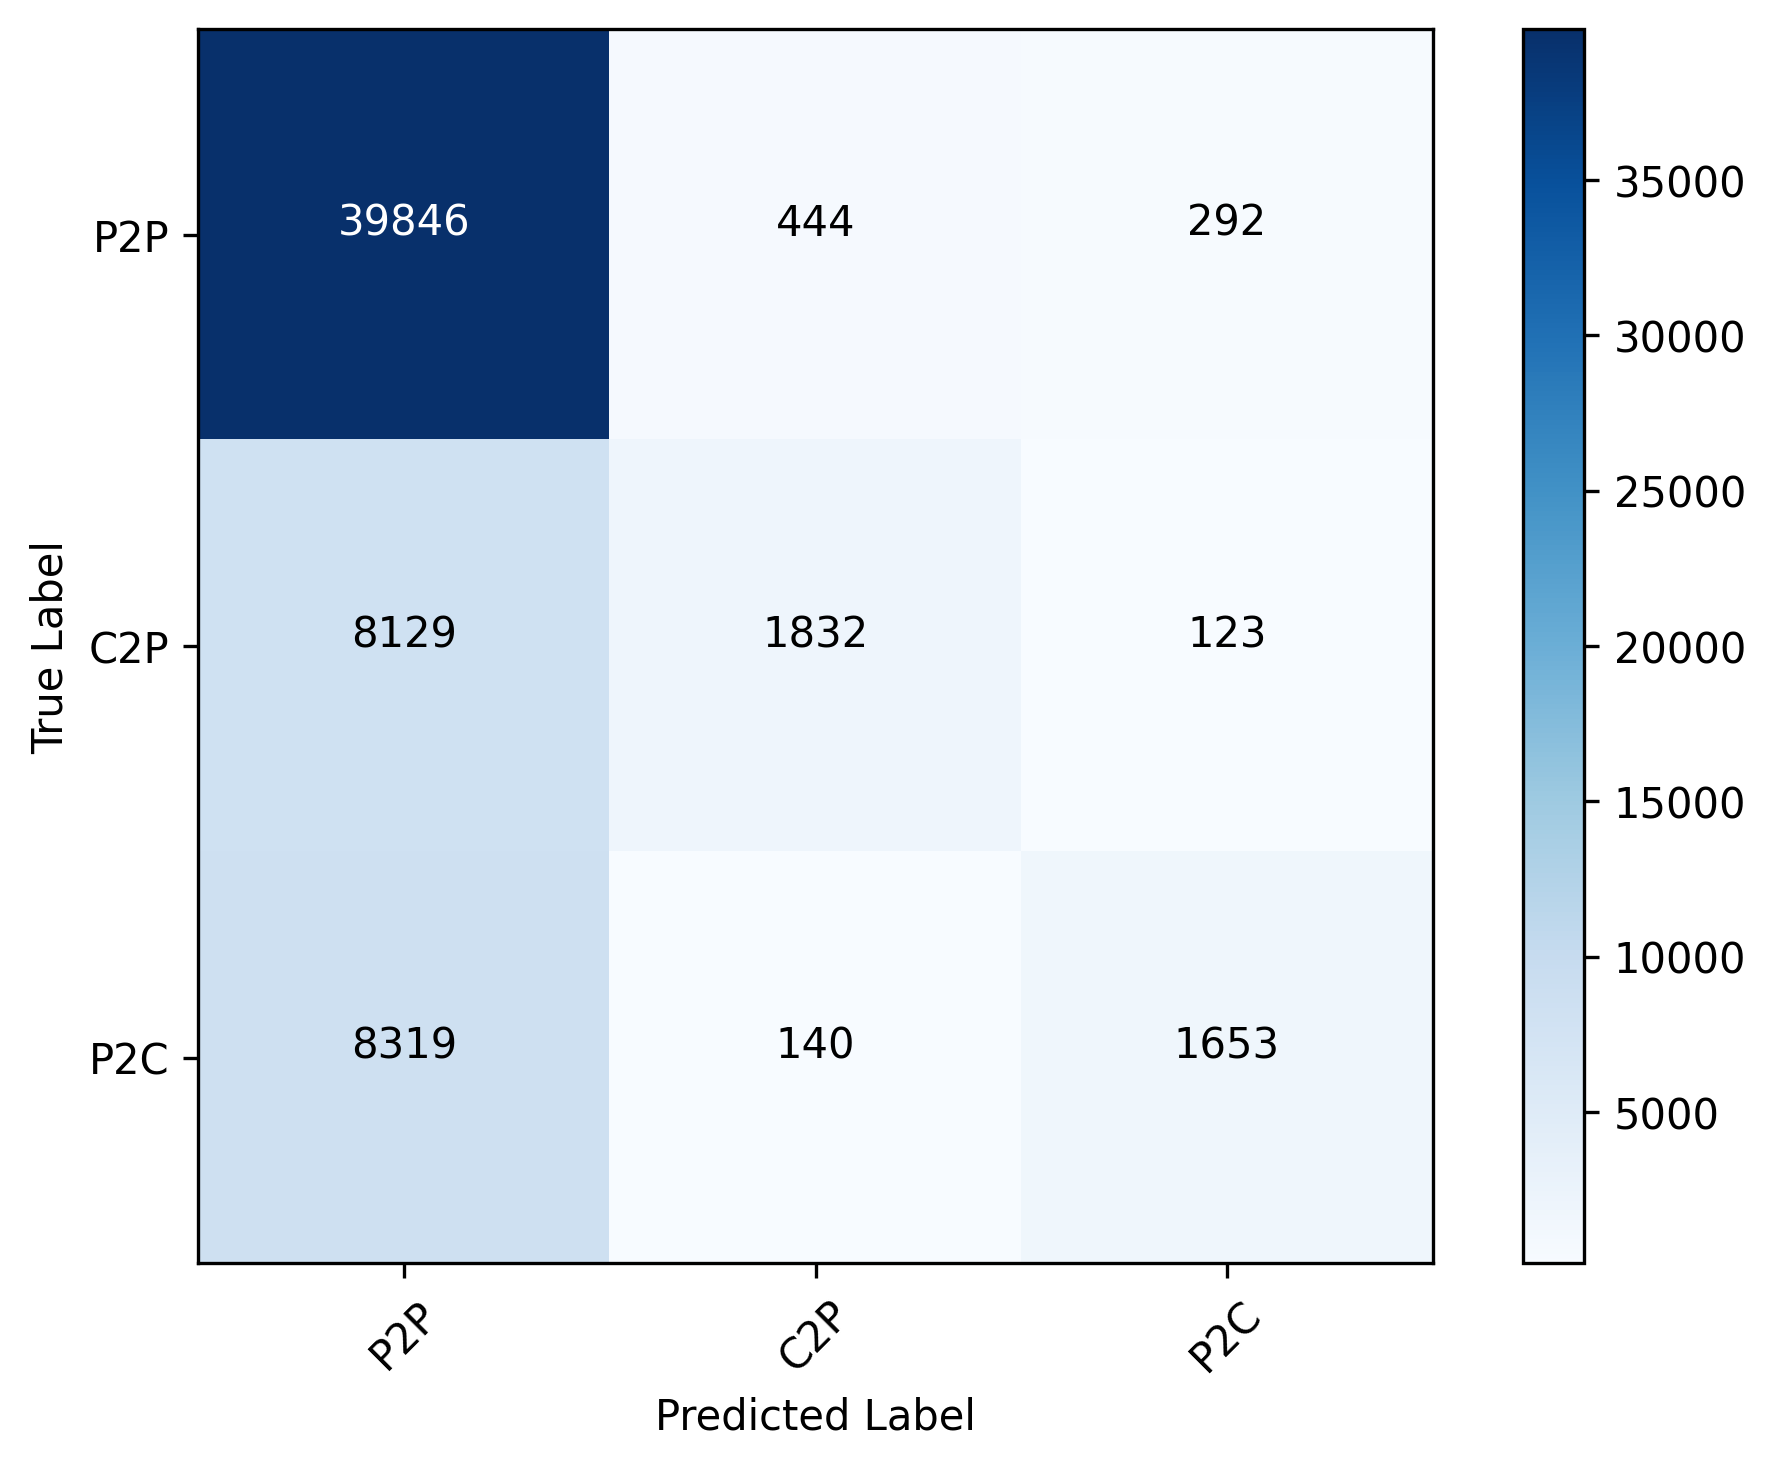
\includegraphics[width=\textwidth]{img/resultados/gnn/partes/caso2_mis_attr/anexo/matriz_confusion/Confusion matrix_febrero_embeddings_ribs_MLP_GAT.png}
%         \caption{GAT + MLP}
%         \label{fig:conf_matrix_gat_mlp}
%     \end{subfigure}

%     \caption{Matrices de confusión obtenidas para el Caso 2 (atributos: creados a partir de dataset de PeeringDB, tarea: predicción de aristas). Se presentan los resultados de las combinaciones de codificador (GCN, GraphSAGE, GAT) con dos tipos de decodificador: producto punto (Dot Product) y MLP.}
%     \label{fig:matrices_confusion_partes_caso2_1millon}
% \end{figure}

% \begin{table}[H]
% \centering
% \begin{tabular}{lcc}
% \hline
% \textbf{Modelo} & \textbf{Decodificador} & \textbf{Accuracy estimada (\%)} \\
% \hline
% GCN & Dot Product & 53.02\% \\
% GraphSAGE & Dot Product & 55.31\% \\
% GAT & Dot Product & 55.21\% \\
% GCN & MLP & 50.71\% \\
% GraphSAGE & MLP & 52.19\% \\
% GAT & MLP & 50.31\% \\
% \hline
% \end{tabular}
% \caption{Accuracy estimada por combinación de codificador y decodificador con \textit{class weight}, es decir, balanceando los pesos de cada clase.}
% \label{tab:accuracy_gnn_1millon_caso2}
% \end{table}

% \subsubsubsection{Resultados Matriz de Confusión}

% A continuación, la Figura \ref{fig:anex:matrices_confusion_experimentos_gnns_decoder} reúne las 24 matrices de confusión normalizadas obtenidas tras entrenar las variantes de GCN, GraphSAGE y GAT con los dos decodificadores (Dot Product y MLP) bajo los cuatro escenarios de entrenamiento con atributos obtenidos del dataset PeeringDB:

















% \subsubsection{Caso 4: Embeddings basados en la predicción de atributos}

% \subsubsubsection{Resultados Matriz de Confusión para PageRank }

% A continuación se presentan las matrices de confusión normalizadas obtenidas con los embeddings generados mediante la inferencia del atributo PageRank de los nodos para los escenarios de entrenamiento evaluados. Puede verse el detalle en la Figura~\ref{fig:mc_pagerank_attr_inf}.\\

% \begin{figure}[H]
%     \centering
%     % GCN pagerank -----------------------------------
%         \begin{subfigure}[b]{0.45\textwidth}
%         \centering
%         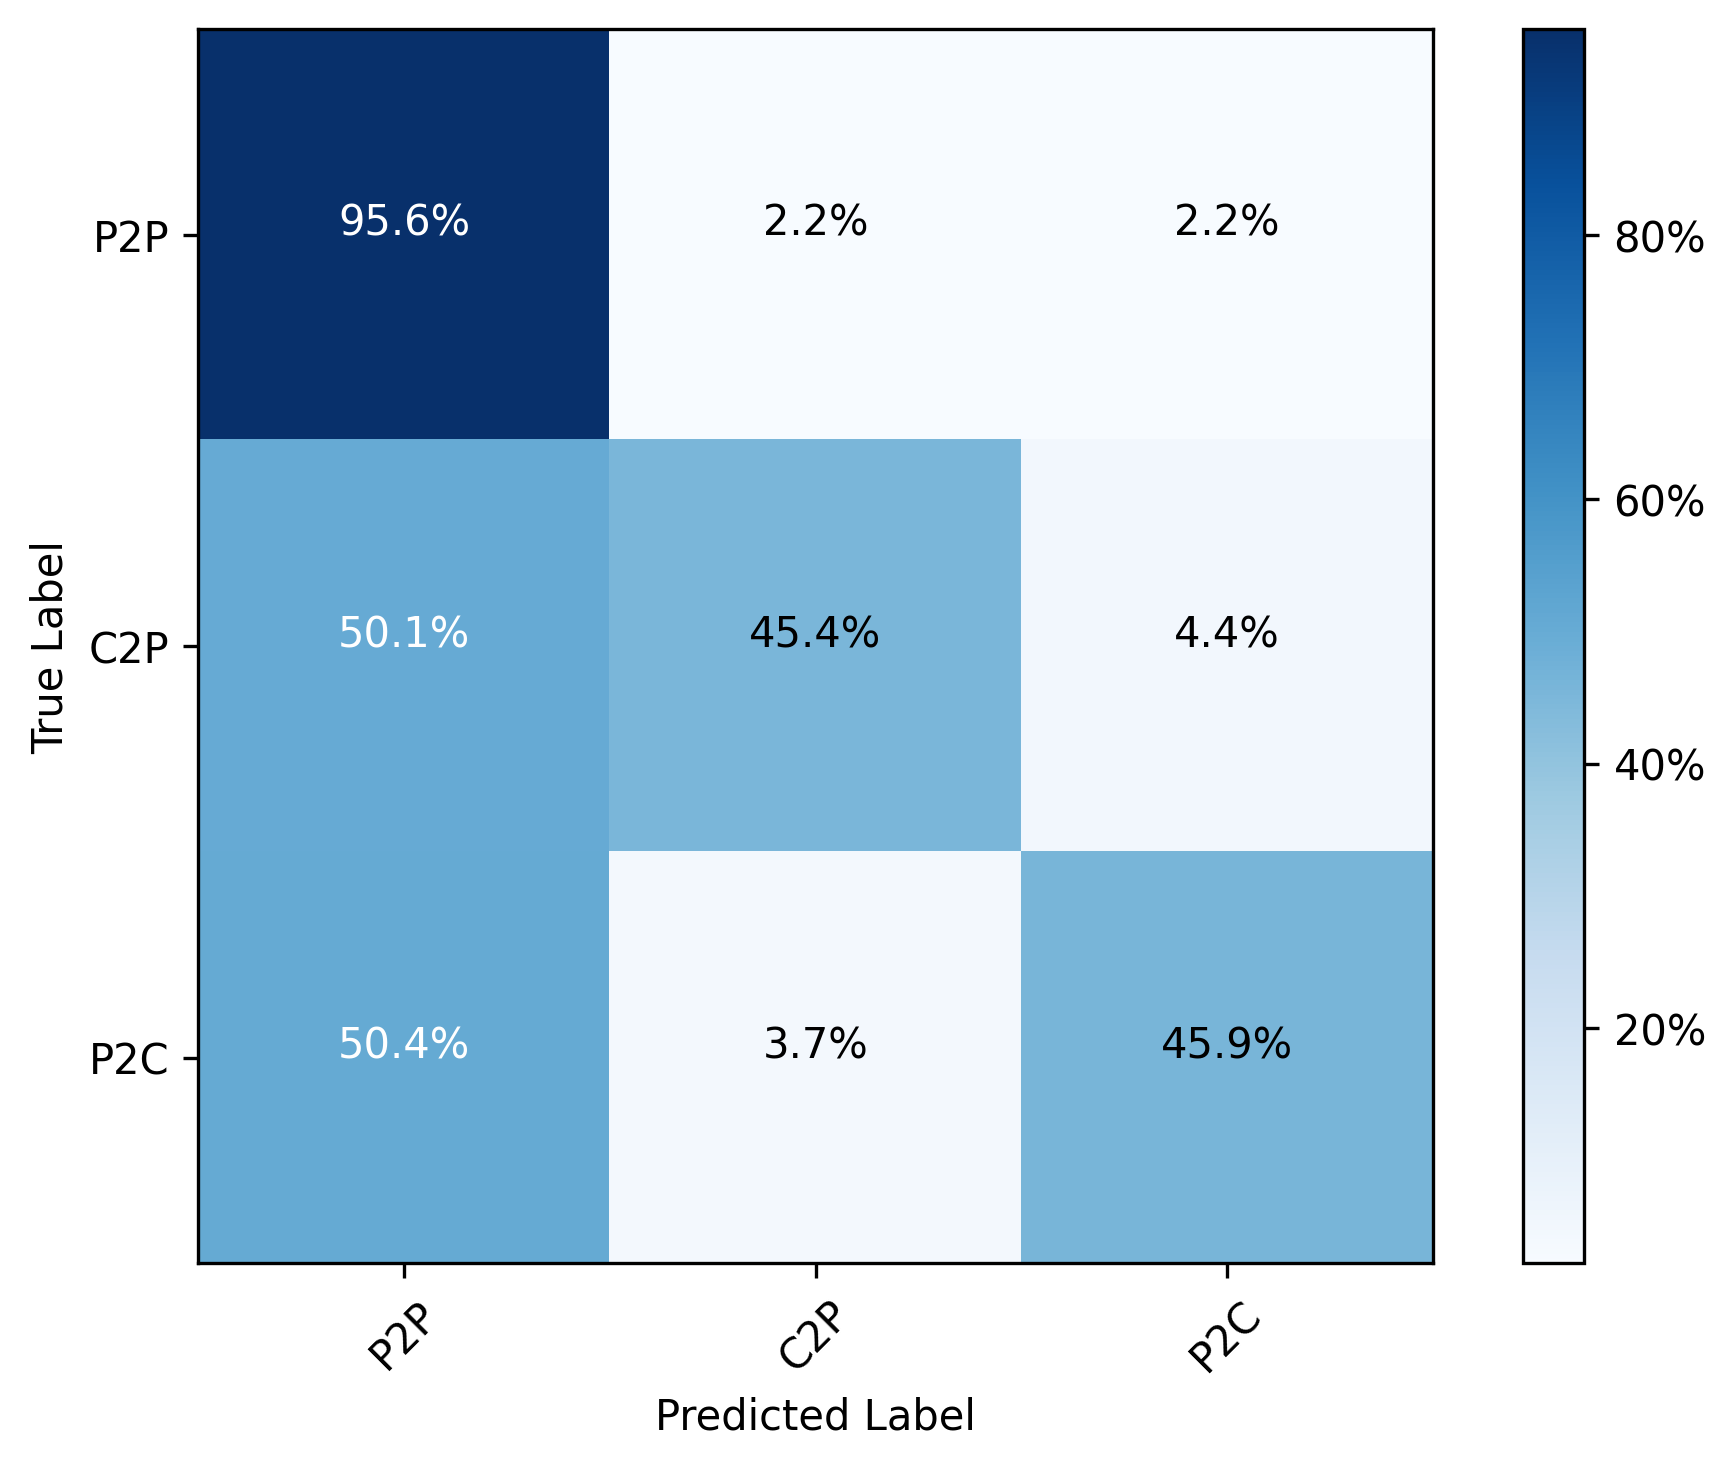
\includegraphics[width=\textwidth]{img/resultados/gnn/partes/caso4_attr_pred/pagerank/Confusion matrix_normalized_febrero_embeddings_ribs_GCN_pagerank_febrero_with_no_batches_with_no_class_weight.png}
%         \caption{GCN - NoW }
%         \label{fig:conf_matrix_gcn_dp}
%     \end{subfigure}
%     \hfill
%     \begin{subfigure}[b]{0.45\textwidth}
%         \centering
%         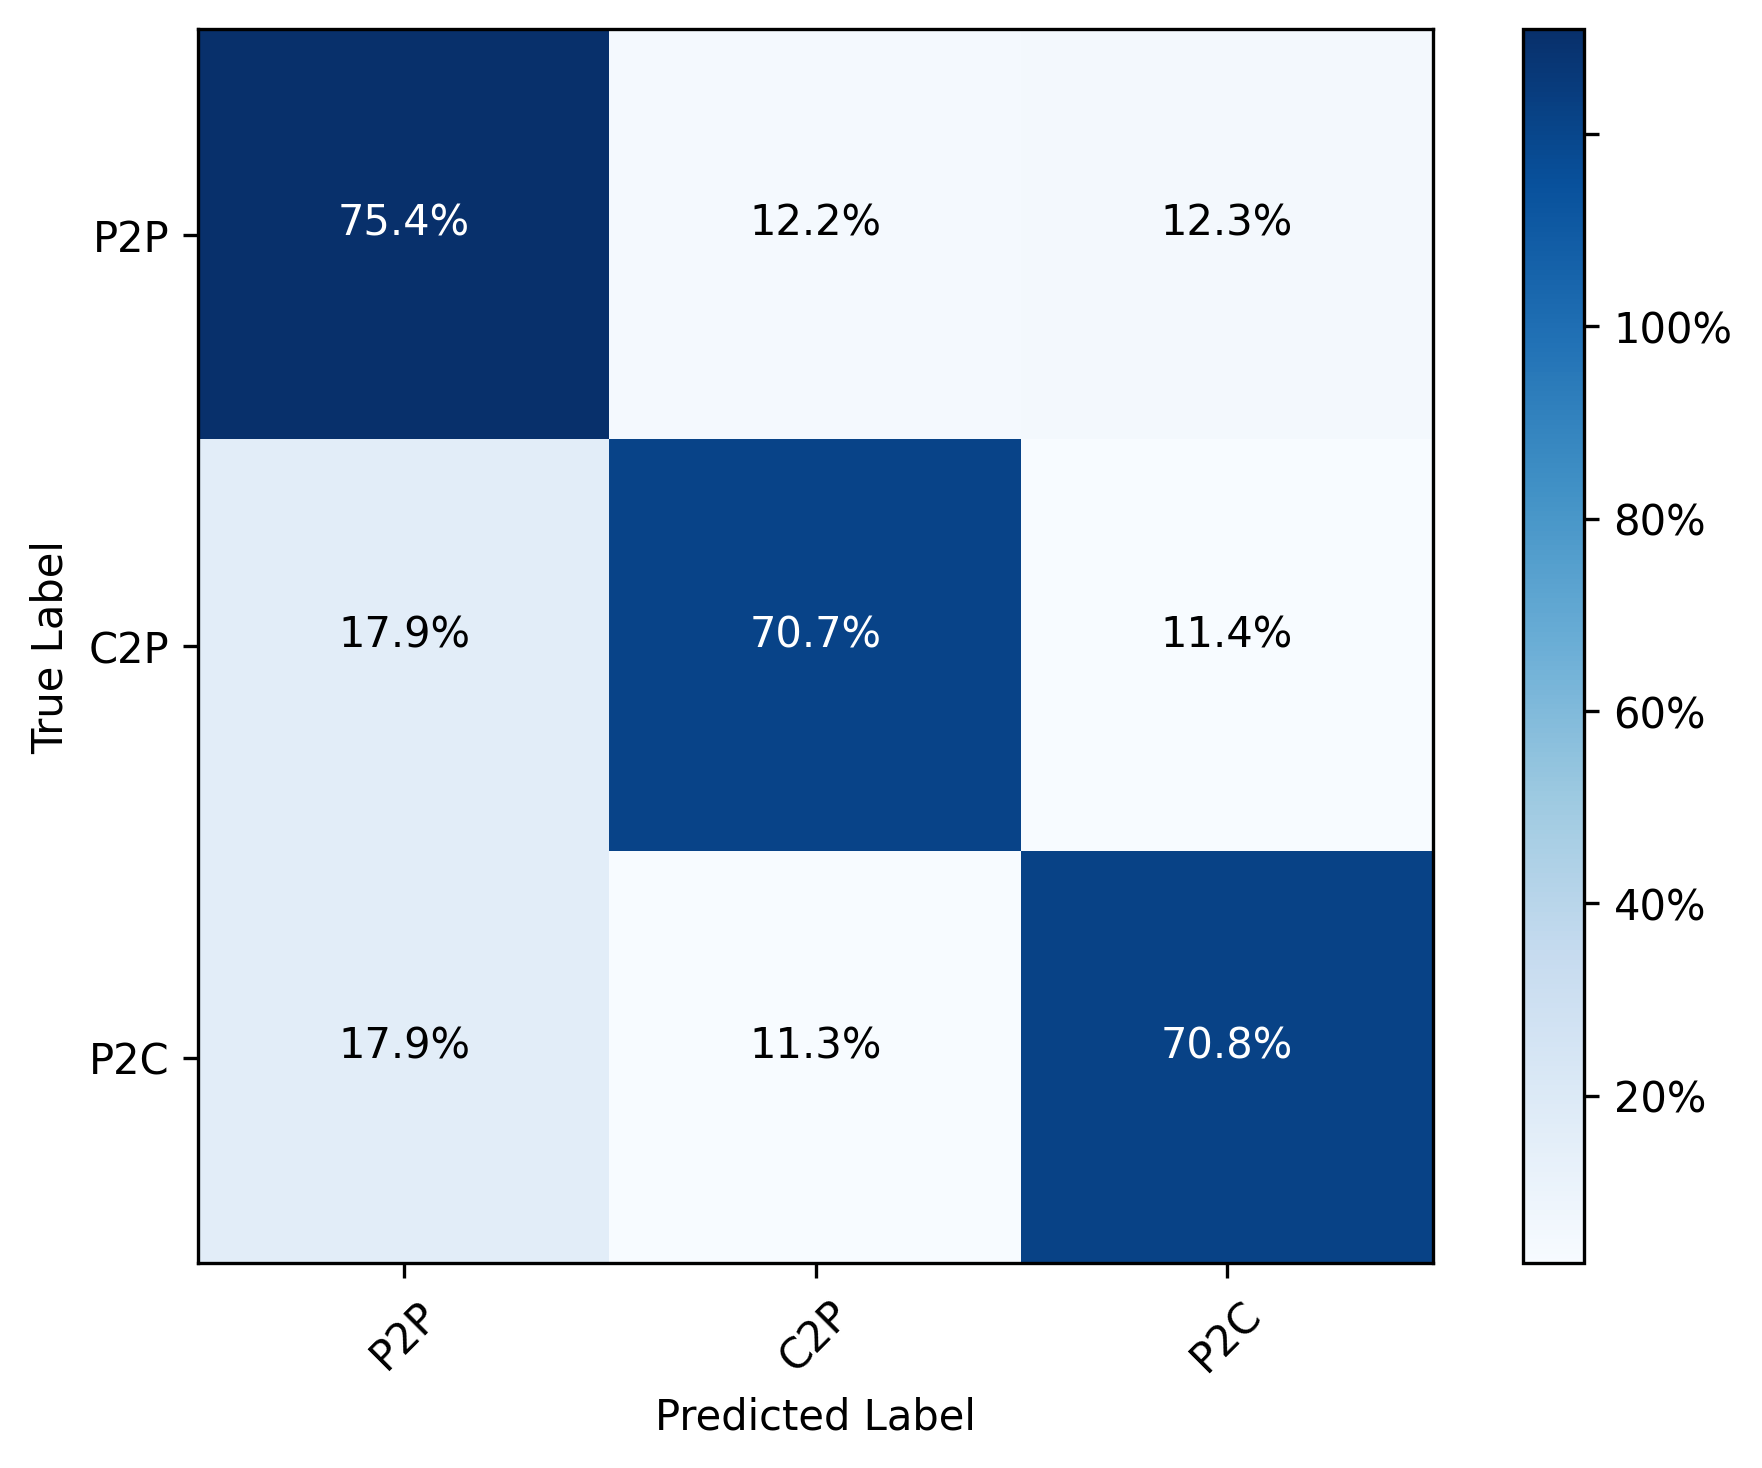
\includegraphics[width=\textwidth]{img/resultados/gnn/partes/caso4_attr_pred//pagerank/Confusion matrix_normalized_febrero_embeddings_ribs_GCN_pagerank_febrero_with_no_batches_with_class_weight.png}
%         \caption{GCN - W}
%         \label{fig:conf_matrix_sage_dp}
%     \end{subfigure}
    
% \end{figure}

% \begin{figure}[H]
%     \centering
%     % GraphSAGE pagerank -----------------------------------
%         \begin{subfigure}[b]{0.45\textwidth}
%         \centering
%         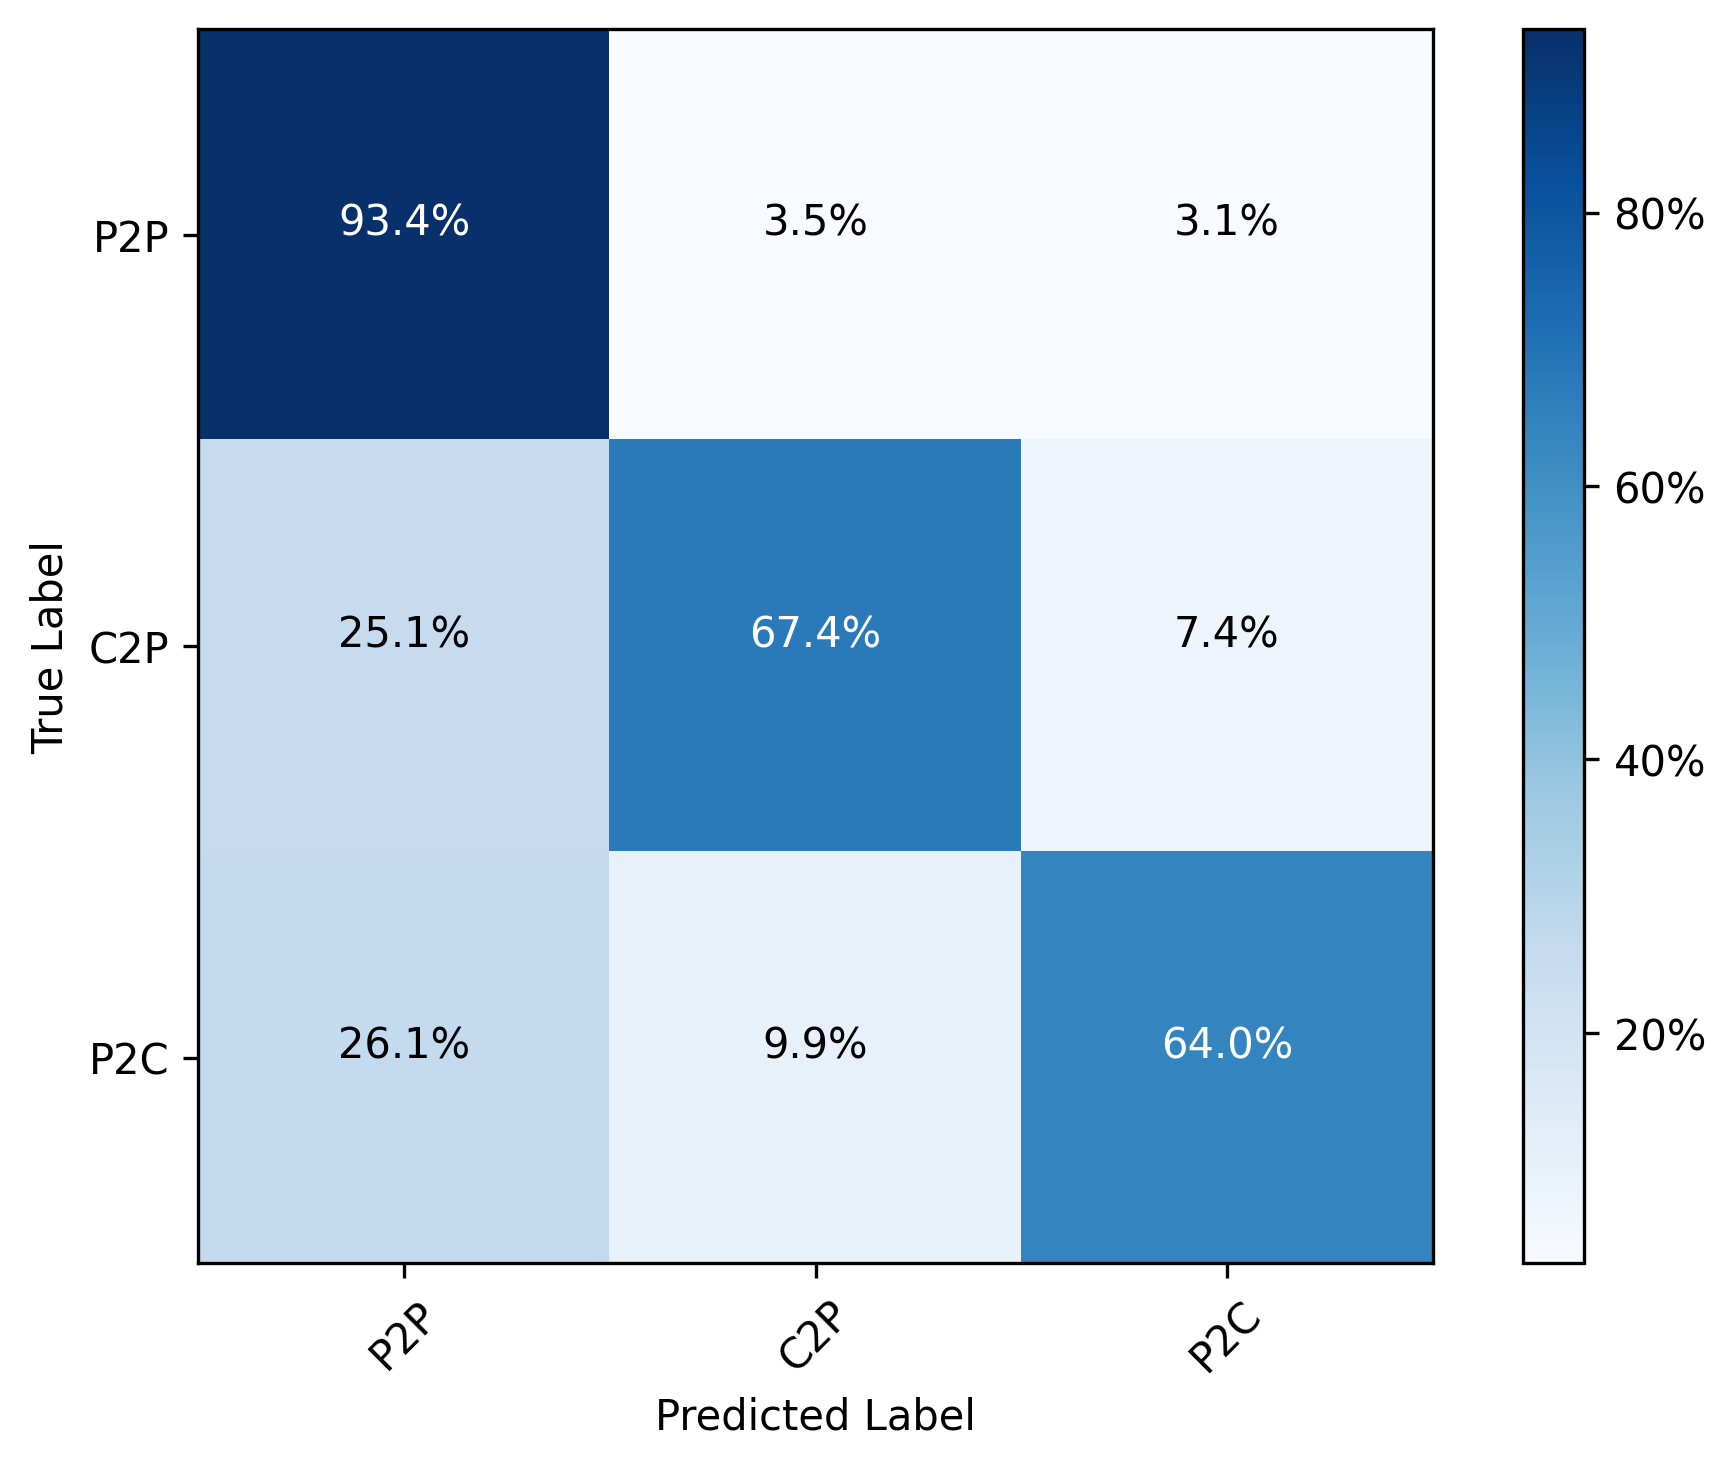
\includegraphics[width=\textwidth]{img/resultados/gnn/partes/caso4_attr_pred/pagerank/Confusion matrix_normalized_febrero_embeddings_ribs_GraphSAGE_pagerank_febrero_with_no_batches_with_no_class_weight.png}
%         \caption{GraphSAGE - NoW }
%         \label{fig:conf_matrix_gcn_dp}
%     \end{subfigure}
%     \hfill
%     \begin{subfigure}[b]{0.45\textwidth}
%         \centering
%         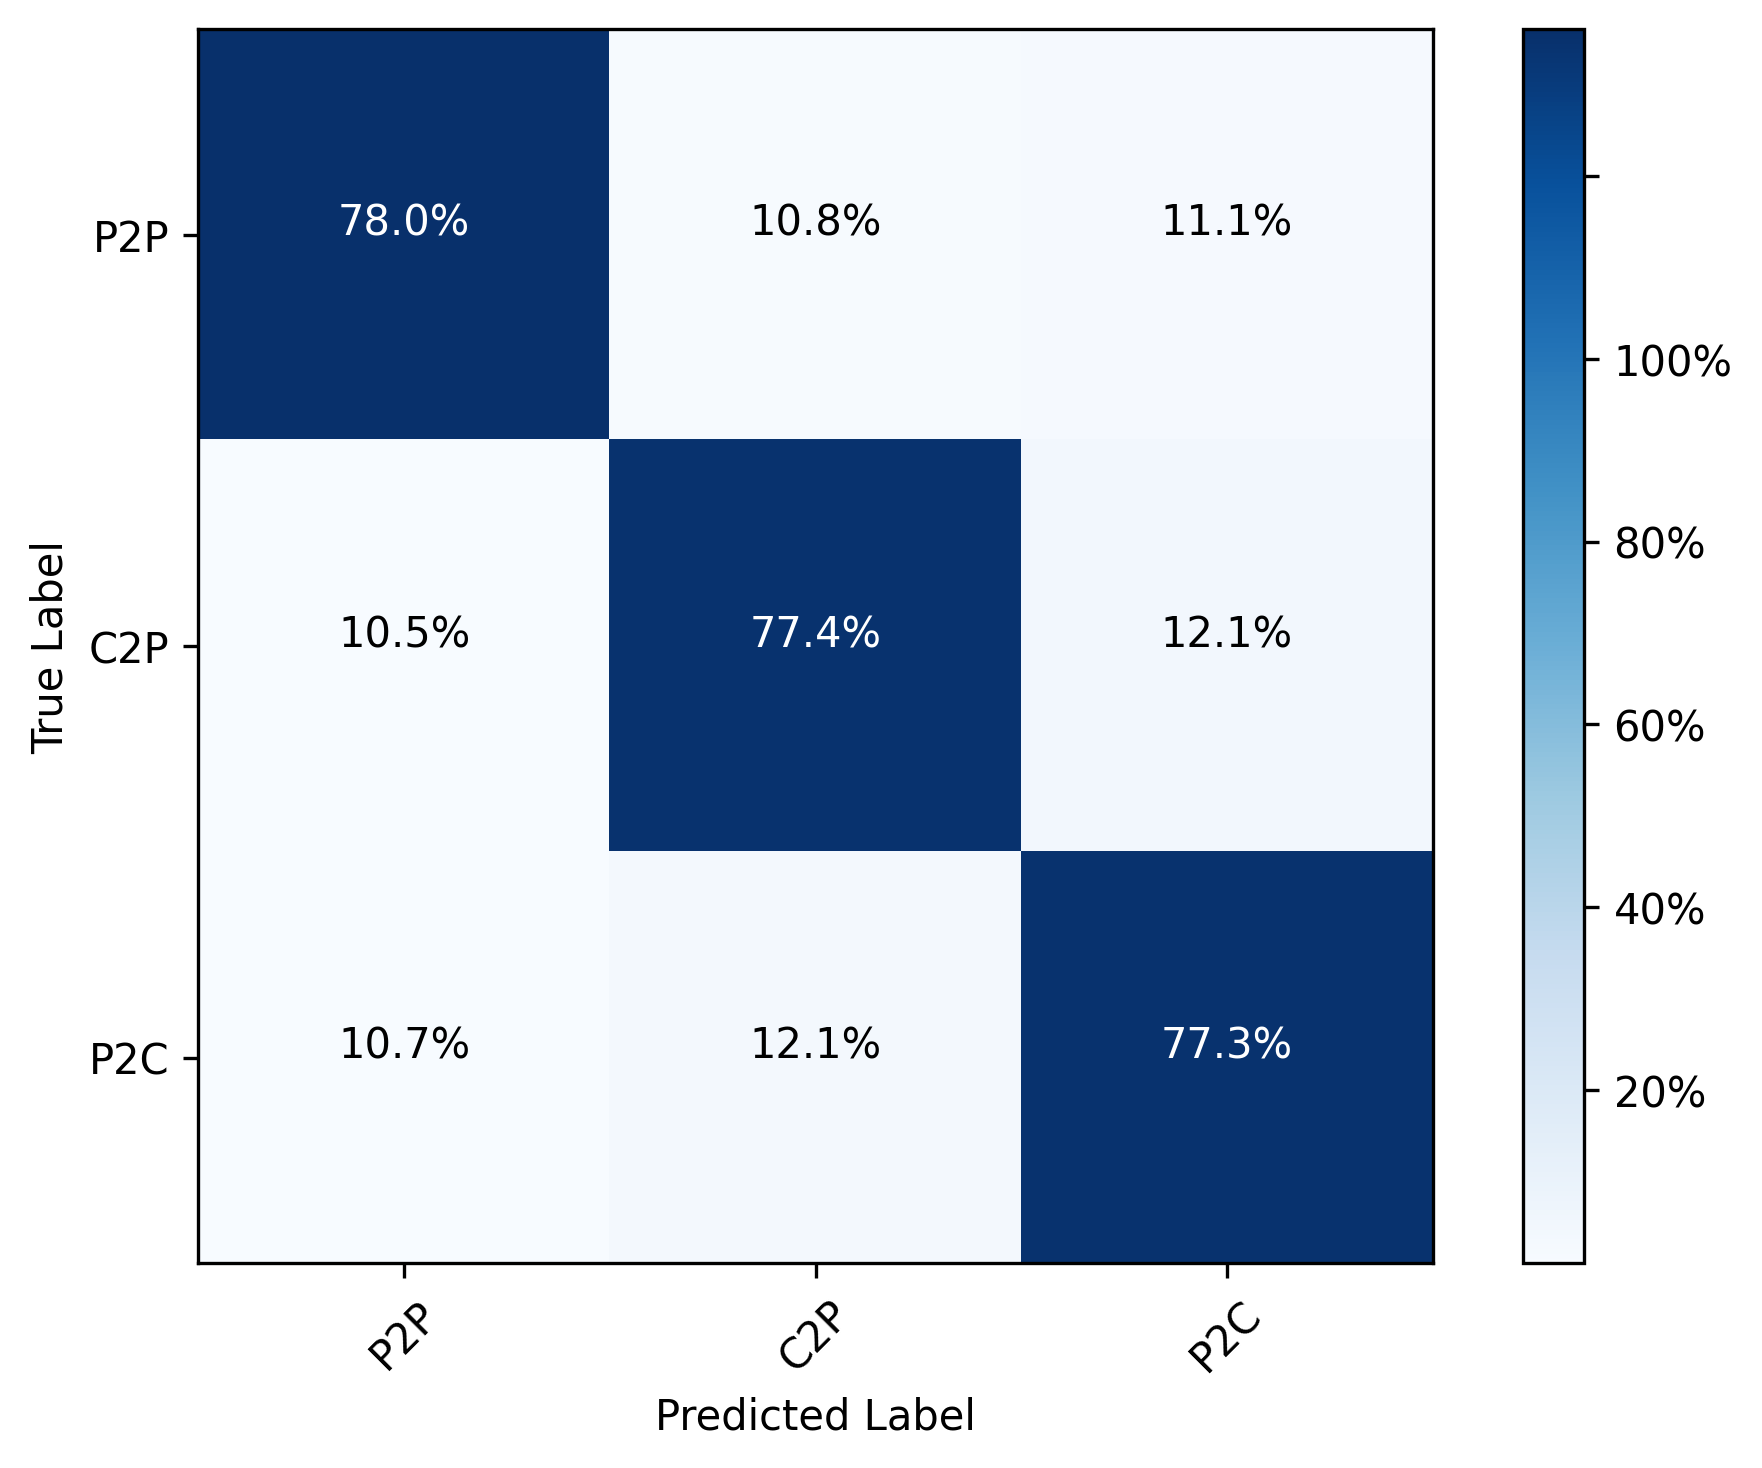
\includegraphics[width=\textwidth]{img/resultados/gnn/partes/caso4_attr_pred//pagerank/Confusion matrix_normalized_febrero_embeddings_ribs_GraphSAGE_pagerank_febrero_with_no_batches_with_class_weight.png}
%         \caption{GraphSAGE - W}
%         \label{fig:conf_matrix_sage_dp}
%     \end{subfigure}
    
% \end{figure}

% \begin{figure}[H]
%     \centering
%     % GAT pagerank -----------------------------------
%         \begin{subfigure}[b]{0.45\textwidth}
%         \centering
%         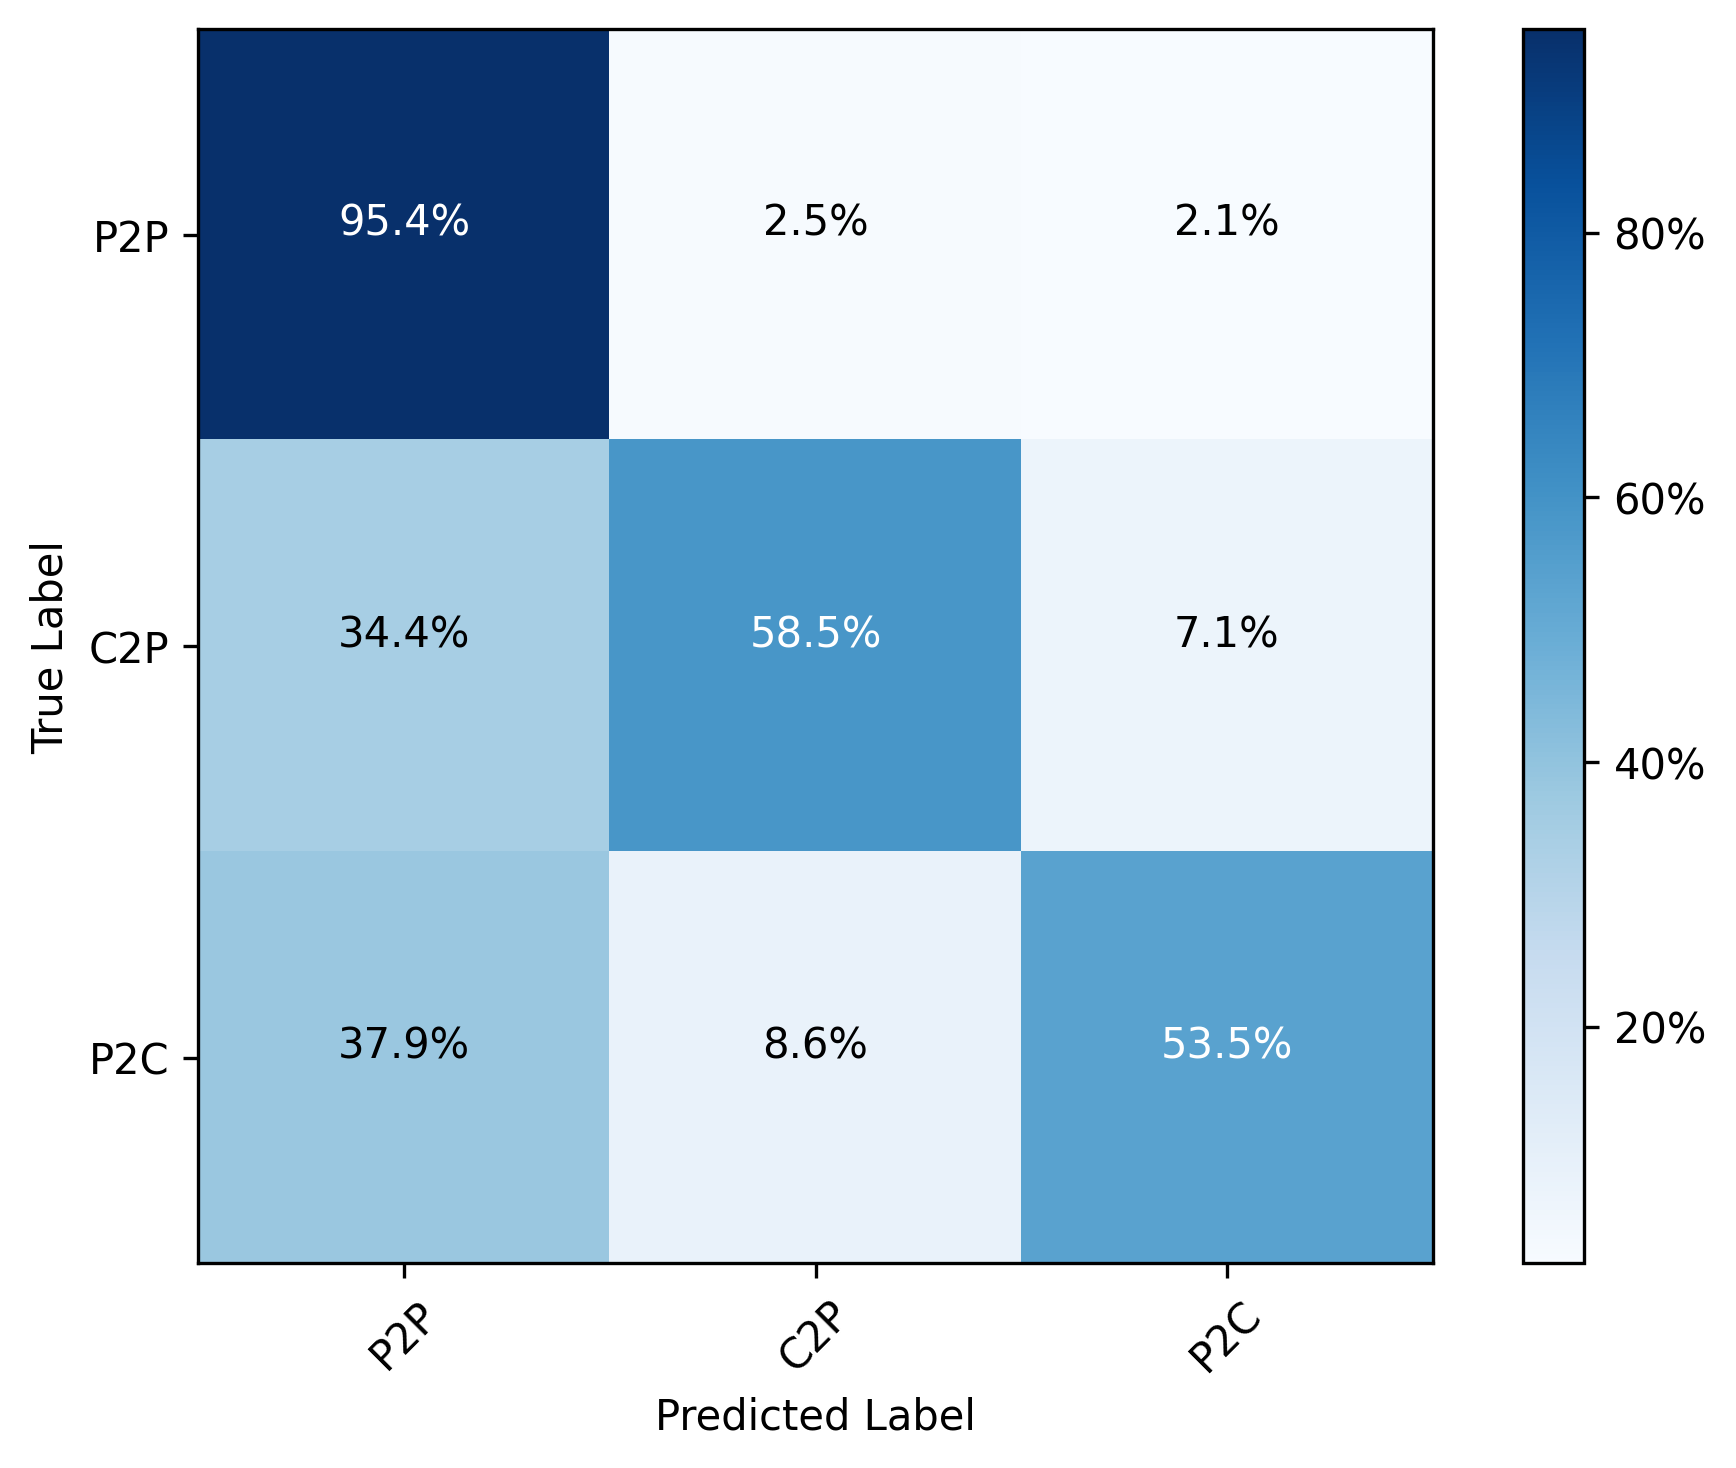
\includegraphics[width=\textwidth]{img/resultados/gnn/partes/caso4_attr_pred/pagerank/Confusion matrix_normalized_febrero_embeddings_ribs_GAT_pagerank_febrero_with_no_batches_with_no_class_weight}
%         \caption{GAT - NoW }
%         \label{fig:conf_matrix_gcn_dp}
%     \end{subfigure}
%     \hfill
%     \begin{subfigure}[b]{0.45\textwidth}
%         \centering
%         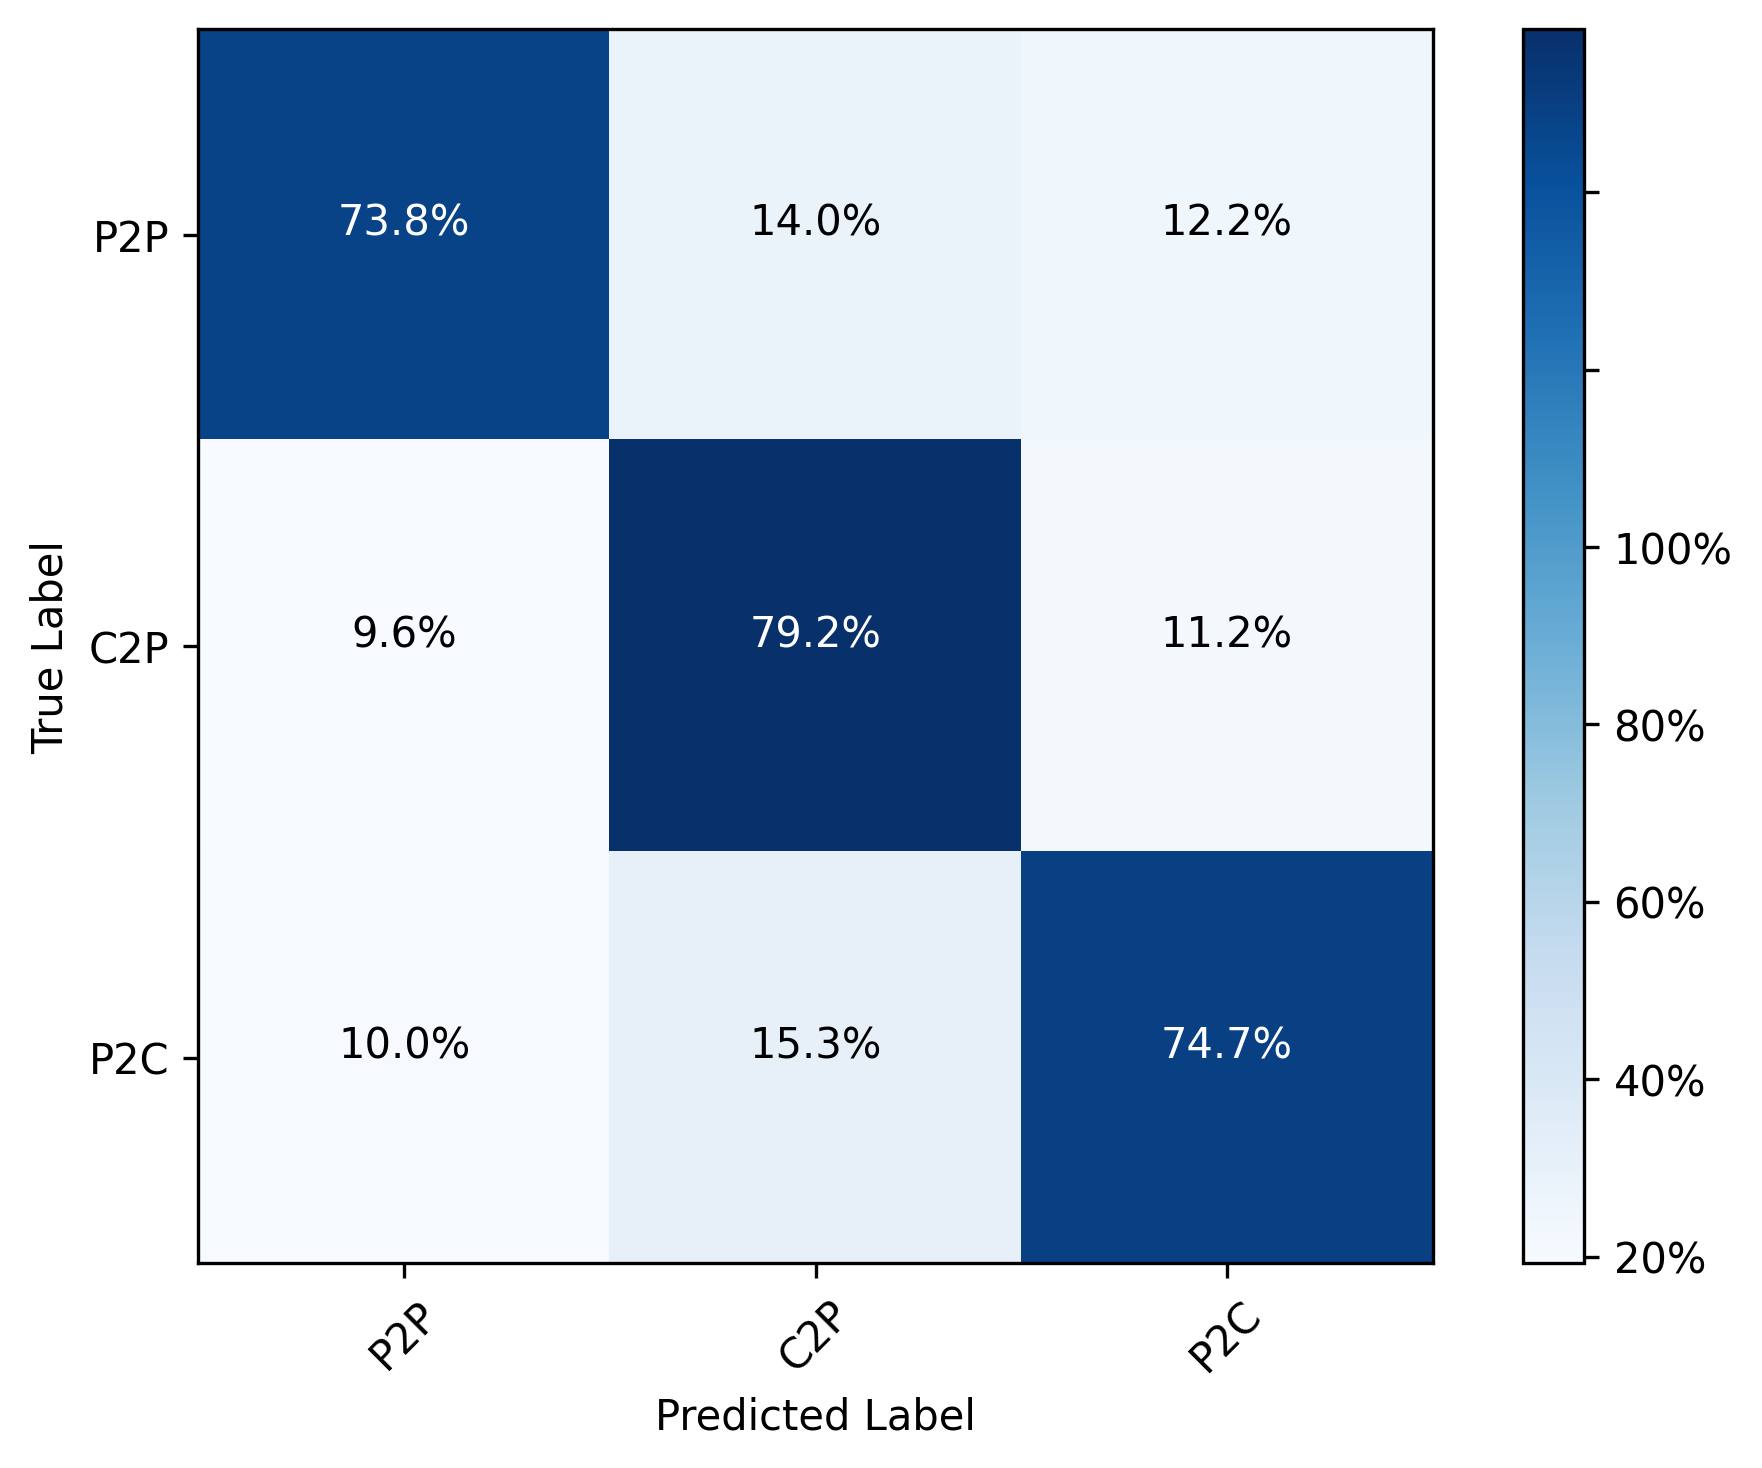
\includegraphics[width=\textwidth]{img/resultados/gnn/partes/caso4_attr_pred/pagerank/Confusion matrix_normalized_febrero_embeddings_ribs_GAT_pagerank_febrero_with_no_batches_with_class_weight}
%         \caption{GAT - W}
%         \label{fig:conf_matrix_sage_dp}
%     \end{subfigure}
    
%     \caption{Matrices de confusión normalizadas basadas en embeddings creados a partir de la predicción del valor de PageRank.
%     Las configuraciones se identifican como \textbf{NoW} (sin balance de clases) y \textbf{W} (con balance de pesos).}
%     \label{fig:mc_pagerank_attr_inf}
% \end{figure}


%\subsubsubsection{Resultados Matriz de Confusión para Degree}

%A continuación se presentan las matrices de confusión normalizadas obtenidas con los embeddings generados mediante la inferencia del grado de nodos para los cuatro escenarios de entrenamiento evaluados. Puede verse el detalle en la Figura~\ref{fig:mc_degree_attr_inf}.\\


% Embdedings creados apartir de la inferencia del grafo d elos nodos

%\begin{figure}[H]
%    \centering
    % GCN pagerank -----------------------------------
 %       \begin{subfigure}[b]{0.45\textwidth}
 %       \centering
        %\includegraphics[width=\textwidth]{img/resultados/gnn/partes/caso4_attr_pred/degree/Confusion matrix_normalized_febrero_embeddings_ribs_GCN_out_degree_febrero_with_no_batches_with_no_class_weight.png}
        %\caption{GCN - NoW }
    %\end{subfigure}
    %\hfill
    %\begin{subfigure}[b]{0.45\textwidth}
    %    \centering
        %\includegraphics[width=\textwidth]{img/resultados/gnn/partes/caso4_attr_pred/degree/Confusion matrix_normalized_febrero_embeddings_ribs_GCN_out_degree_febrero_with_no_batches_with_class_weight.png}
     %   5\caption{GCN - W}
    %\end{subfigure}
    

%\end{figure}
%\begin{figure}[H]
%    \centering
    % GraphSAGE pagerank -----------------------------------
 %       \begin{subfigure}[b]{0.45\textwidth}
  %      \centering
        %\includegraphics[width=\textwidth]{img/resultados/gnn/partes/caso4_attr_pred/degree/Confusion matrix_normalized_febrero_embeddings_ribs_GraphSAGE_out_degree_febrero_with_no_batches_with_no_class_weight.png}
        %\caption{GraphSAGE - NoW }
    %\end{subfigure}
    %\hfill
    %\begin{subfigure}[b]{0.45\textwidth}
    %    \centering
        %\includegraphics[width=\textwidth]{img/resultados/gnn/partes/caso4_attr_pred/degree/Confusion matrix_normalized_febrero_embeddings_ribs_GraphSAGE_out_degree_febrero_with_no_batches_with_class_weight.png}
        %\caption{GraphSAGE - W}
    %\end{subfigure}
    

%\end{figure}
%\begin{figure}[H]
%    \centering
    % GAT pagerank -----------------------------------
 %       \begin{subfigure}[b]{0.45\textwidth}
  %      \centering
        %\includegraphics[width=\textwidth]{img/resultados/gnn/partes/caso4_attr_pred/degree/Confusion matrix_normalized_febrero_embeddings_ribs_GAT_out_degree_febrero_with_no_batches_with_no_class_weight}
        %\caption{GAT - NoW }
    %\end{subfigure}
    %\hfill
    %\begin{subfigure}[b]{0.45\textwidth}
     %   \centering
        %\includegraphics[width=\textwidth]{img/resultados/gnn/partes/caso4_attr_pred/degree/Confusion matrix_normalized_febrero_embeddings_ribs_GAT_out_degree_febrero_with_no_batches_with_class_weight}
   %     \caption{GAT - W}
  %  \end{subfigure}
    
 %   \caption{Matrices de confusión normalizadas basado en embeddings creados  apartir de prediccion valor de PageRank.
   % Las configuraciones se identifican como \textbf{NoW} (sin balance de clases), \textbf{W} (con balance de pesos).}
 %   \label{fig:mc_degree_attr_inf}
%\end{figure}


%//////////////////////////////////////
%\subsubsection{Caso 4: Embeddings generados mediante DeepWalk con predicción de enlaces}
%\subsubsubsection{Resultados Matriz de Confusión}



%A continuación se presentan las matrices de confusión normalizadas obtenidas con los embeddings generados mediante DeepWalk para los cuatro escenarios de entrenamiento evaluados. Puede verse el detalle en la Figura~\ref{fig:conf_matrices_deepwalk_full}.\\



%\begin{figure}[H]
%    \centering
    % Primera fila ───────────────────────────────────────────
%    \begin{subfigure}[b]{0.24\textwidth}
%        \centering
        %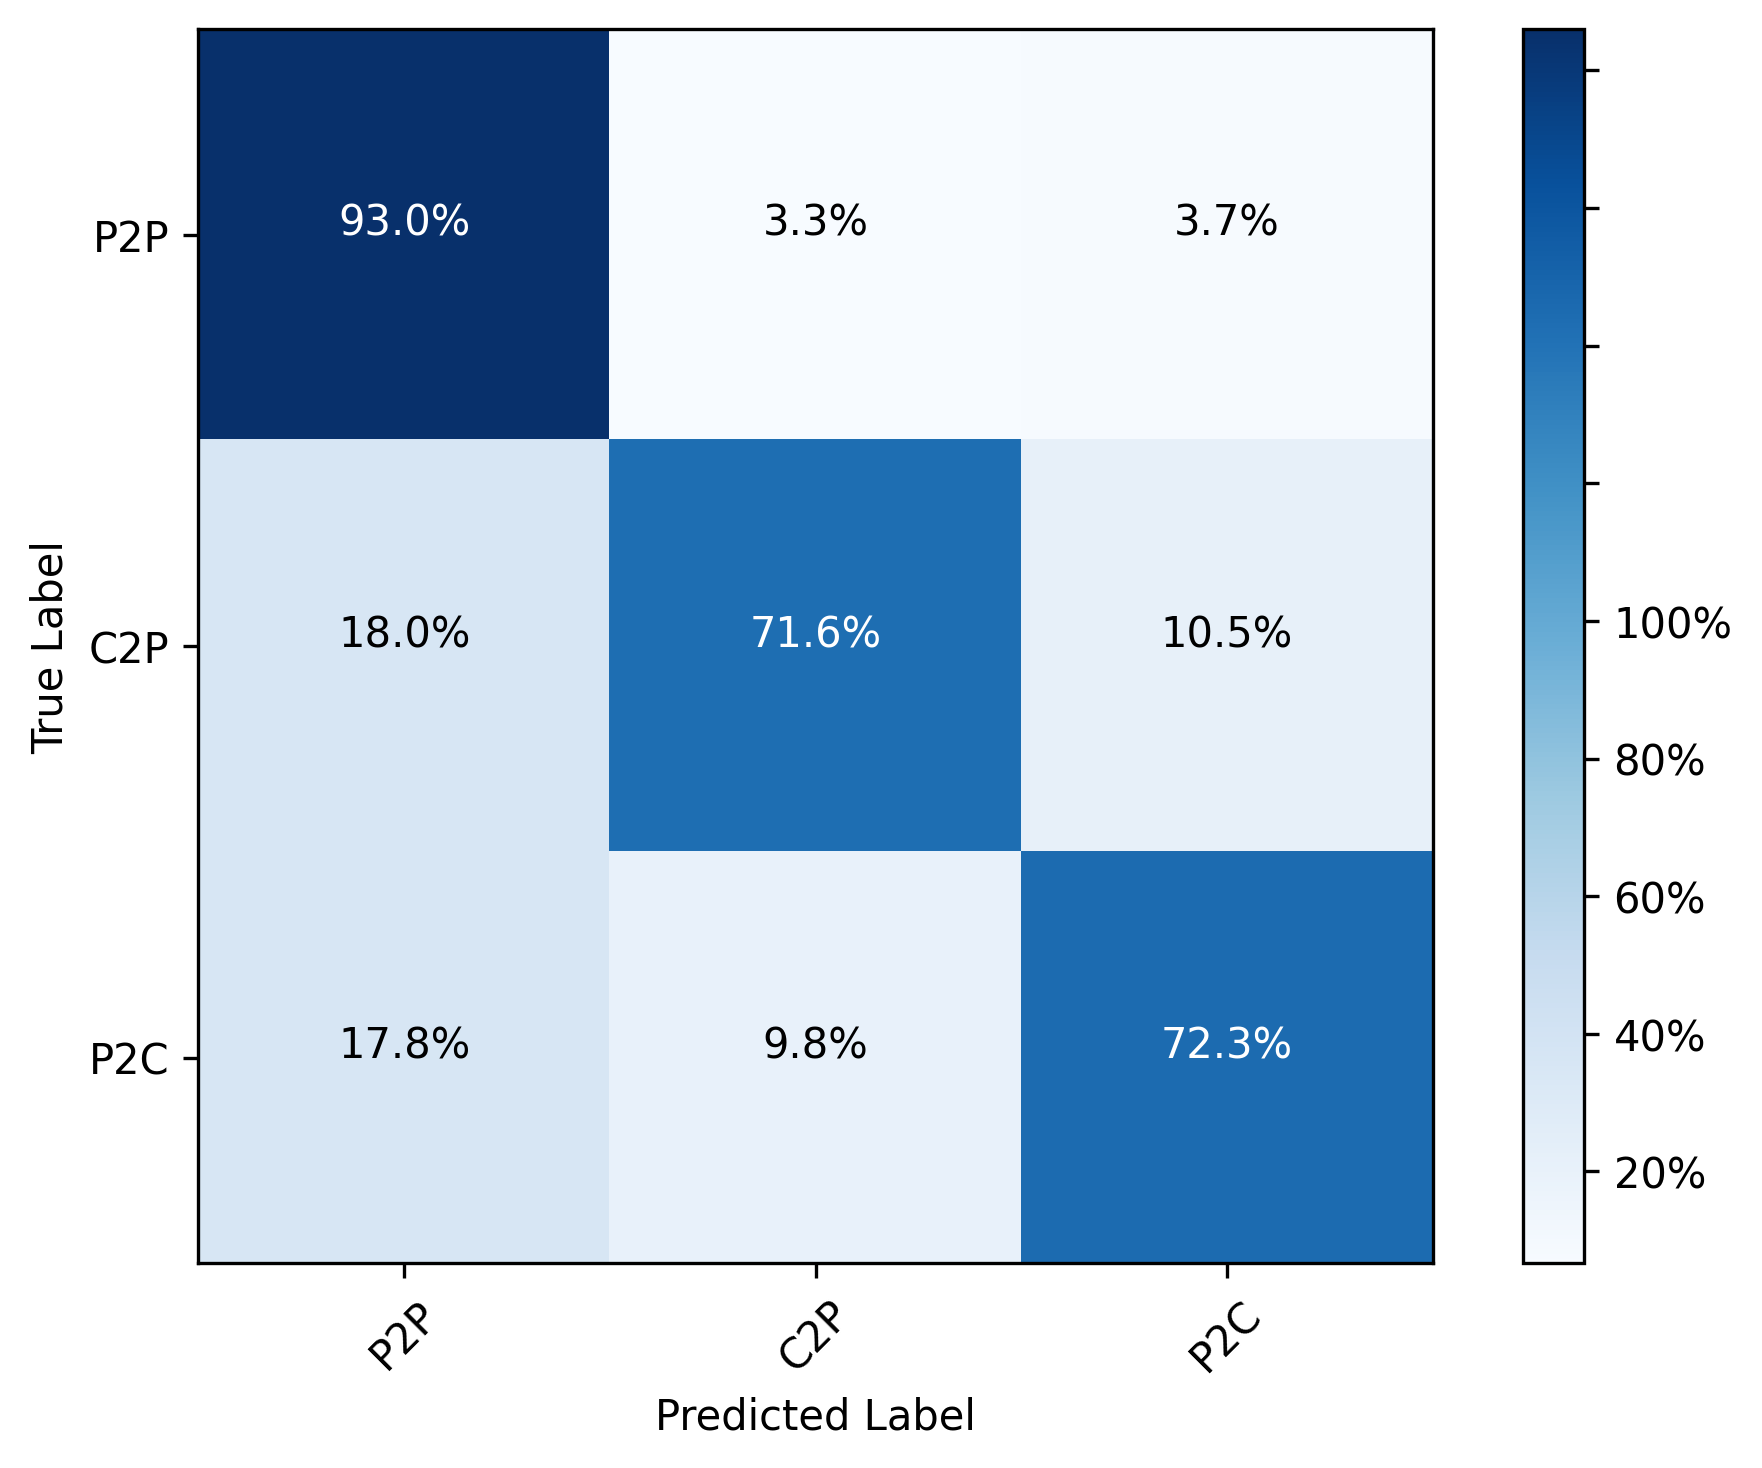
\includegraphics[width=\textwidth]{img/resultados/gnn/partes/caso2_mis_attr/resultados/matriz_confusion/deepwalk/Confusion matrix_normalized_febrero_embeddings_deepWalk_febrero_with_no_batches_with_no_class_weight.png}
        %\caption{NoBatch-NoW}
        %\label{fig:conf_matrix_deepwalk_nobatch_now}
    %\end{subfigure}
    %\hfill
    %\begin{subfigure}[b]{0.24\textwidth}
     %   \centering
        %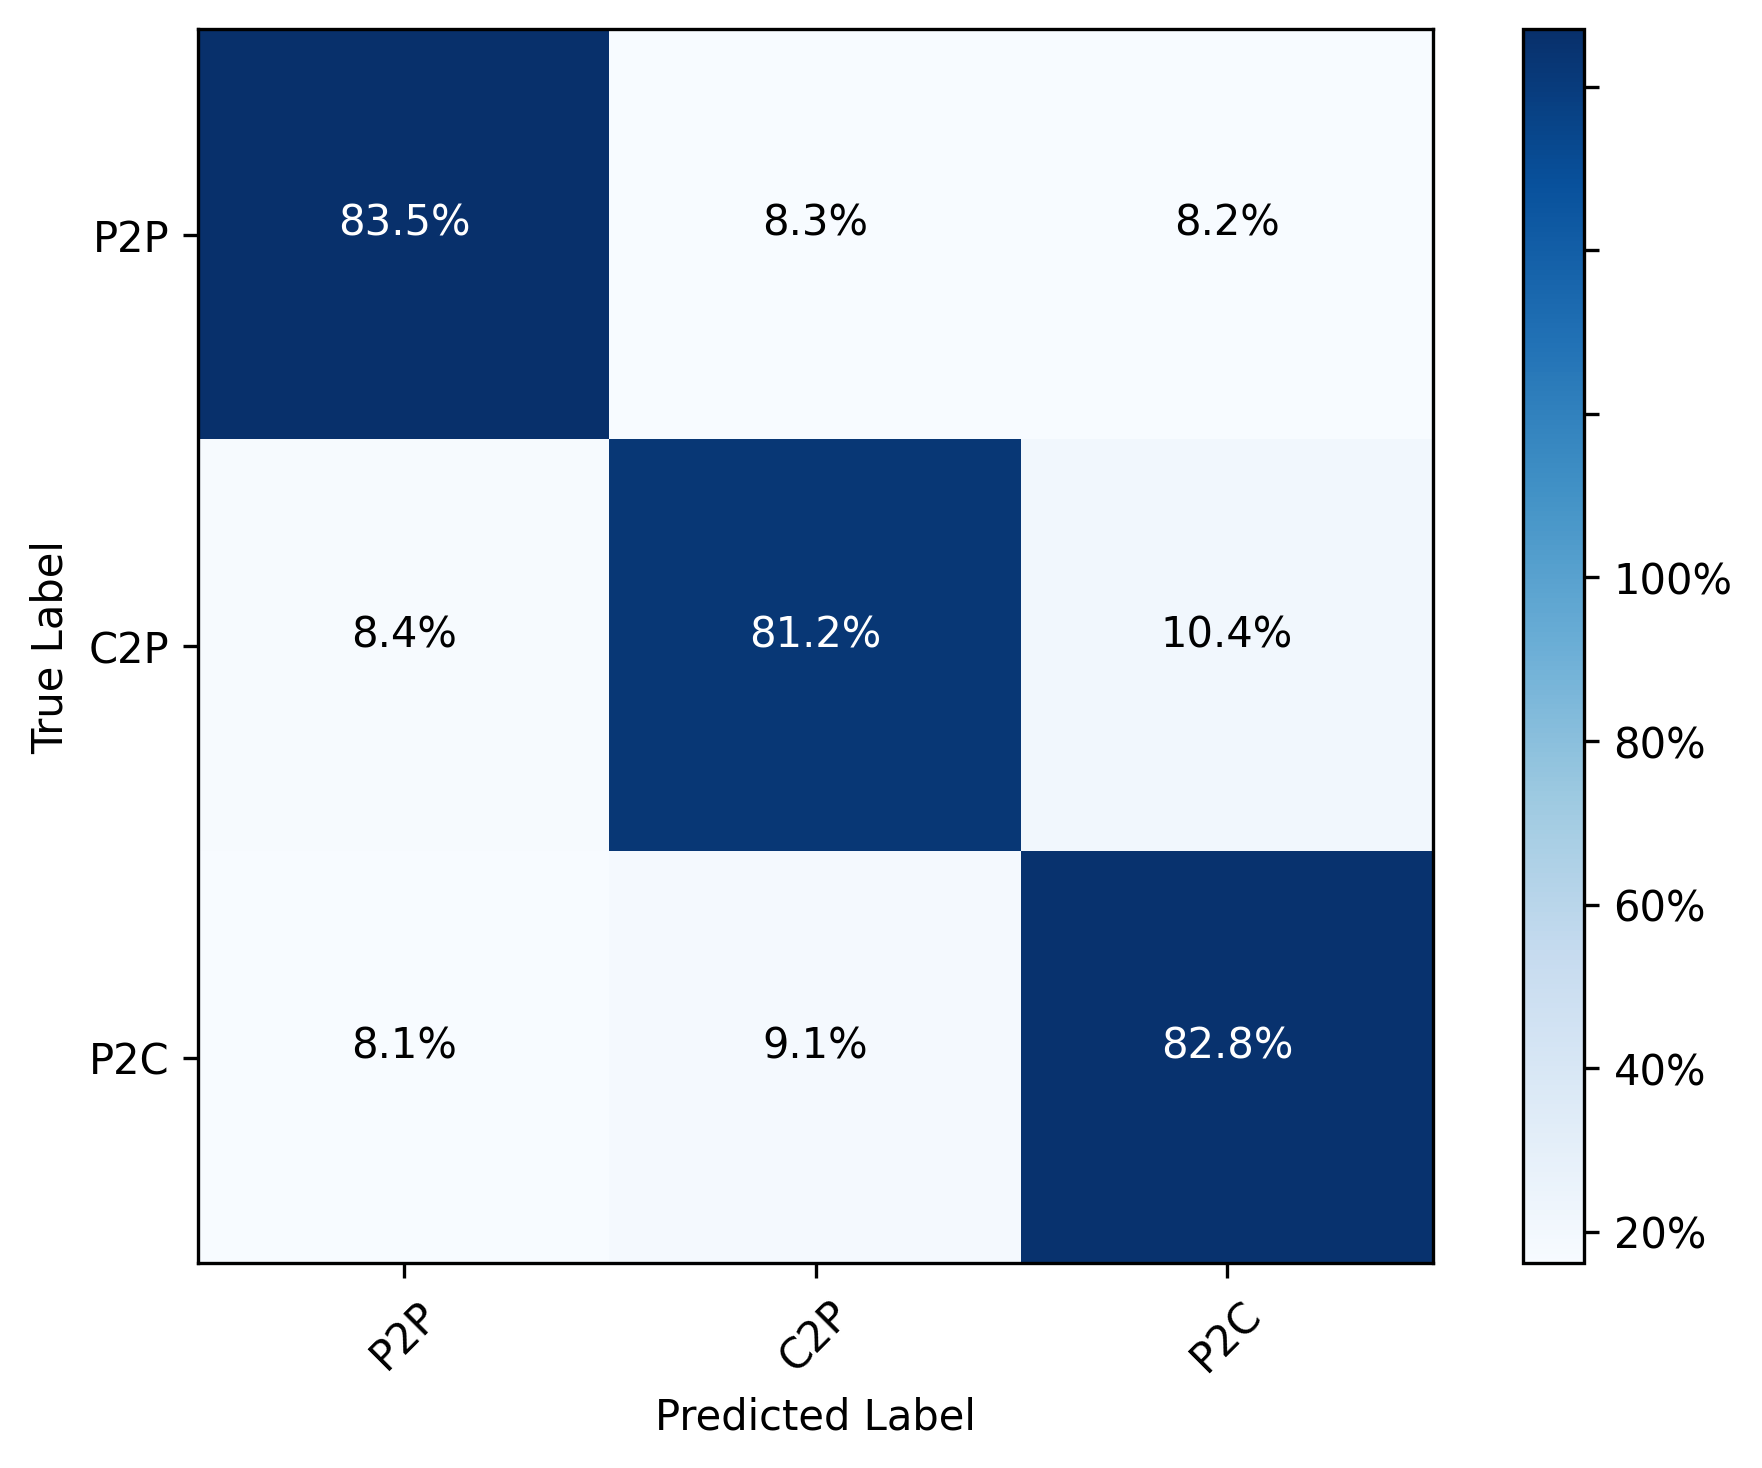
\includegraphics[width=\textwidth]{img/resultados/gnn/partes/caso2_mis_attr/resultados/matriz_confusion/deepwalk/Confusion matrix_normalized_febrero_embeddings_deepWalk_febrero_with_no_batches_with_class_weight.png}
        %\caption{NoBatch-W}
        %\label{fig:conf_matrix_deepwalk_nobatch_w}
    %\end{subfigure}
    %\hfill
    %\begin{subfigure}[b]{0.24\textwidth}
    %    \centering
        %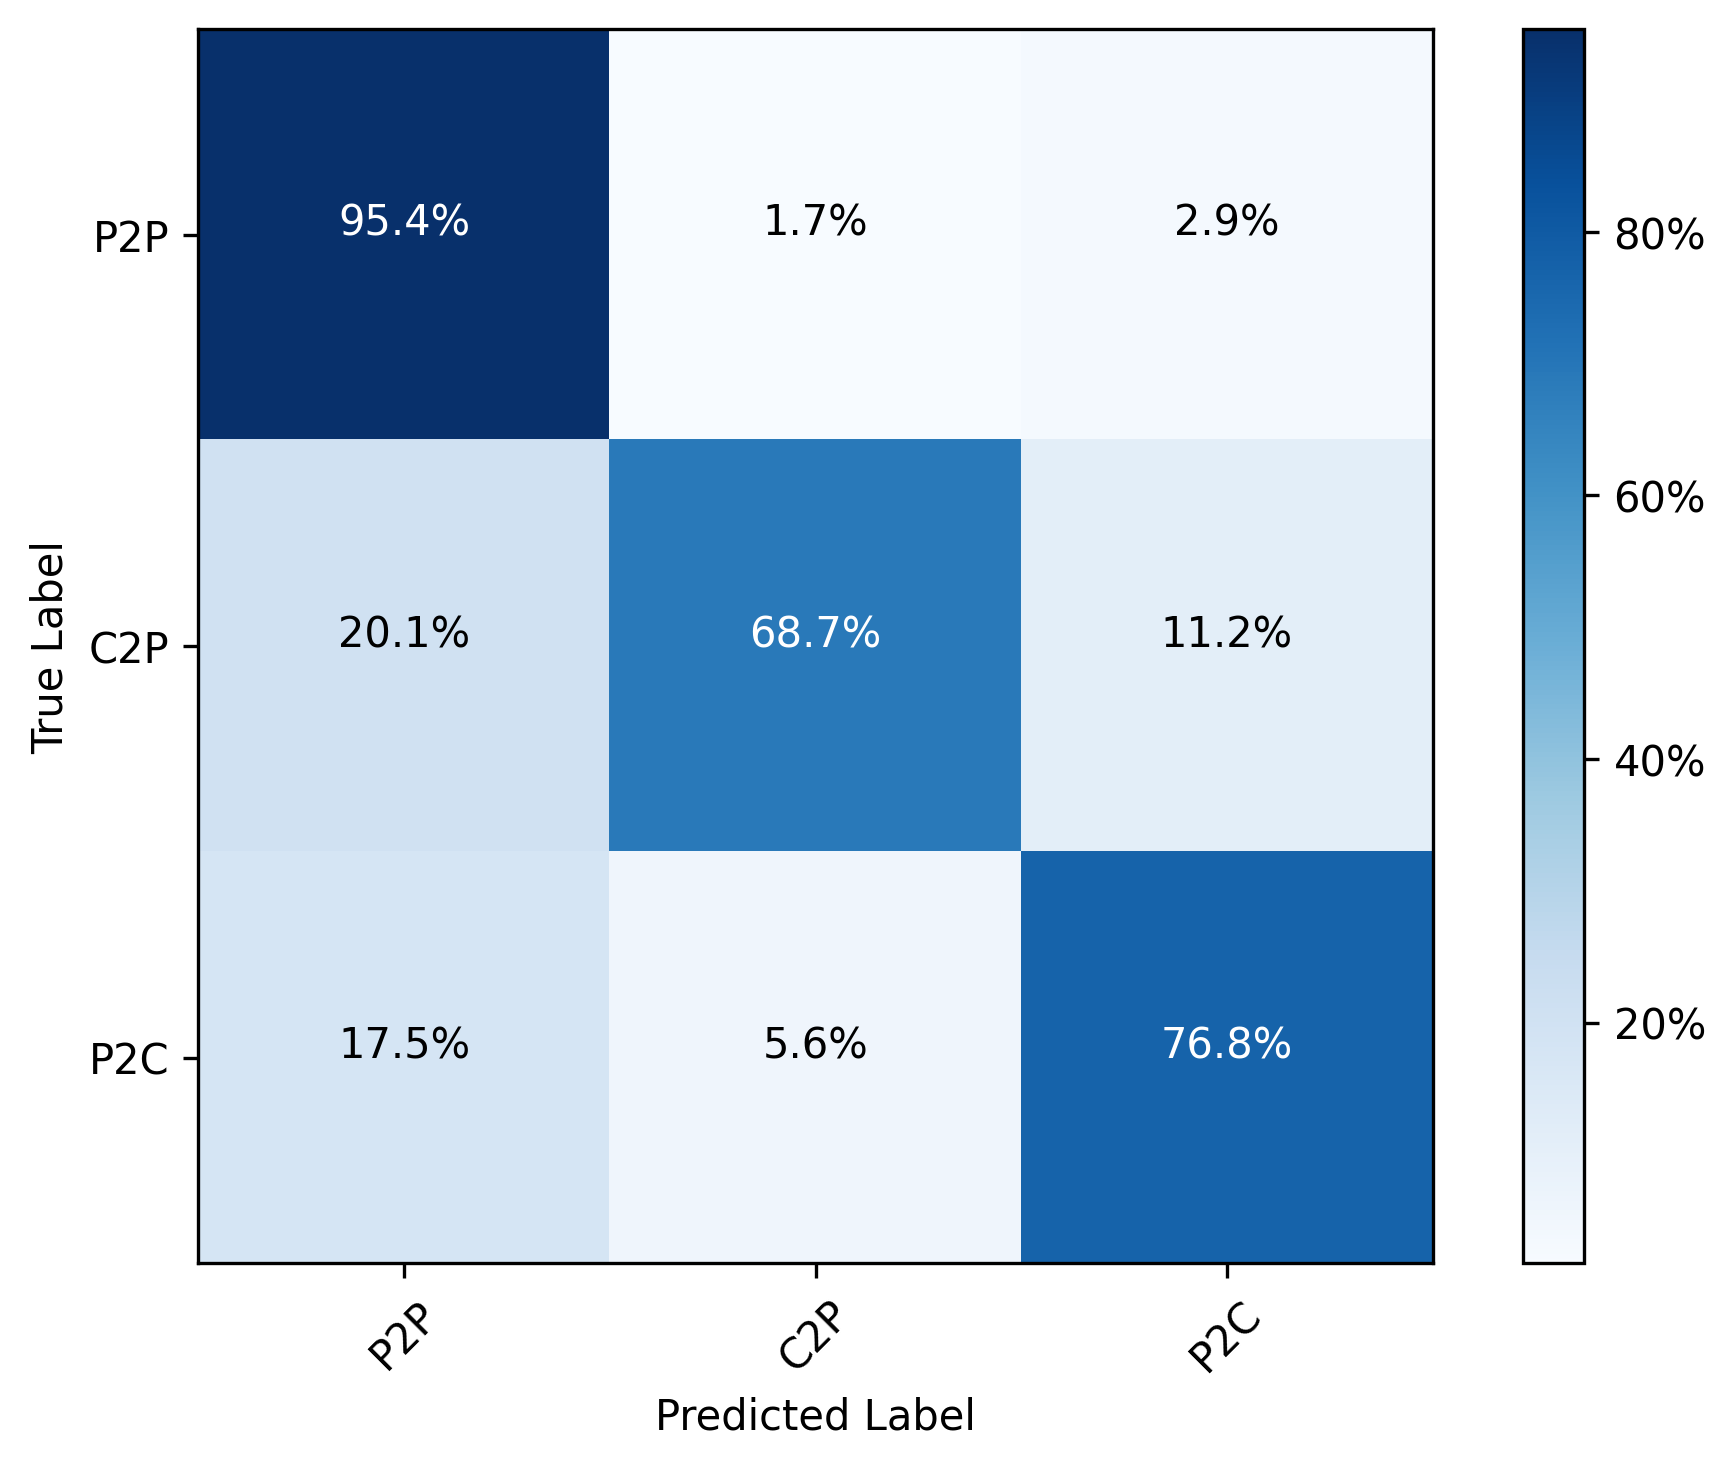
\includegraphics[width=\textwidth]{img/resultados/gnn/partes/caso2_mis_attr/resultados/matriz_confusion/deepwalk/Confusion matrix_normalized_febrero_embeddings_deepWalk_febrero_with_batches_with_no_class_weight.png}
        %\caption{Batch-NoW}
        %\label{fig:conf_matrix_deepwalk_batch_now}
    %\end{subfigure}
    %\hfill
    %\begin{subfigure}[b]{0.24\textwidth}
    %    \centering
        %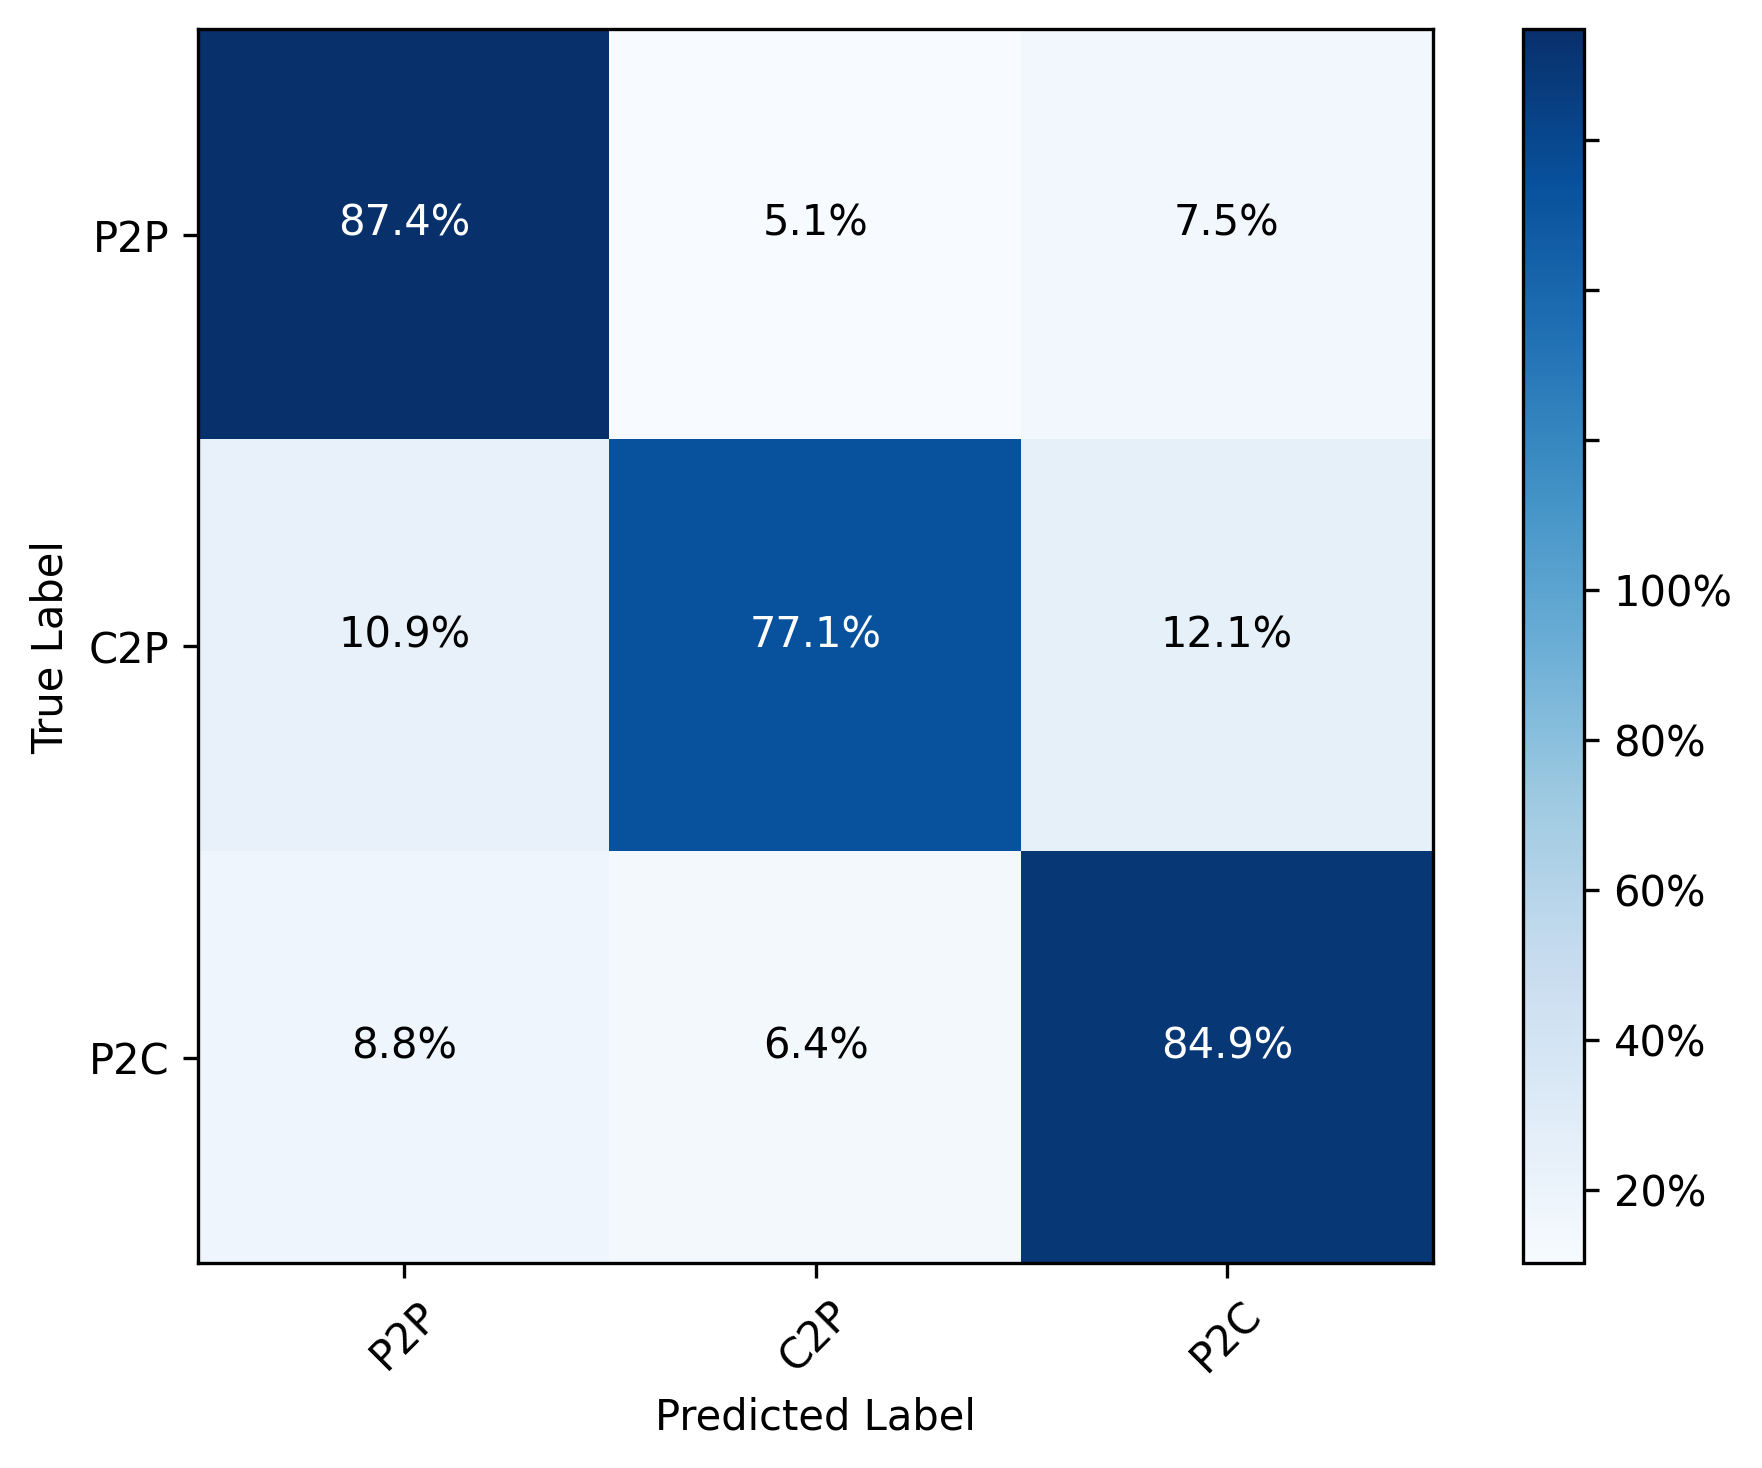
\includegraphics[width=\textwidth]{img/resultados/gnn/partes/caso2_mis_attr/resultados/matriz_confusion/deepwalk/Confusion matrix_normalized_febrero_embeddings_deepWalk_febrero_with_batches_with_class_weight.png}
        %\caption{Batch-W}
        %\label{fig:conf_matrix_deepwalk_batch_w}
    %\end{subfigure}

    %\caption{Matrices de confusión normalizadas para los cuatro escenarios de entrenamiento con embeddings DeepWalk:  
    %\textbf{NoBatch-NoW} – sin mini-batching ni pesos de clase;  
    %\textbf{NoBatch-W} – sin mini-batching con pesos de clase;  
    %\textbf{Batch-NoW} – con mini-batching sin pesos de clase;  
    %\textbf{Batch-W} – con mini-batching y pesos de clase.}
    %\label{fig:conf_matrices_deepwalk_full}
%\end{figure}






%\subsubsection{ Caso 5: Embeddings generados mediante BGP2Vec} \label{sec:anexo_bgp2vec_emb}



%Un experimento adicional que se realizó consistió en crear erróneamente el diccionario de IDs a embeddings. Como resultado, el modelo alcanzó una precisión de 81.54\%. A continuación, se presentan los resultados obtenidos para este caso, donde se muestran tanto la curva de precisión como la matriz de confusión. En la Figura~\ref{fig:acc-bgp2vc-idnaqver}, se observa el gráfico de la precisión durante el entrenamiento y la prueba, mientras que en la Figura~\ref{fig:mc-bgp2vc-idnaqvr} se presenta la matriz de confusión correspondiente.\\ 


%\begin{figure}[H]
%    \centering
%    \begin{minipage}{0.5\linewidth}
%        \centering
       
        %
\includegraphics[width=\linewidth]{img/resultados/gnn/partes/casobgp2vec/acc_bgp2_vc_idnaqver.png}
     %   \caption{Gráfico de la precisión (accuracy) del modelo con embeddings creados a partir de BGP2Vec para el caso de IDNA, durante el entrenamiento y la prueba.}
    %    \label{fig:acc-bgp2vc-idnaqver}
   % \end{minipage}%
    %\begin{minipage}{0.5\linewidth}
        %\centering
        %
\includegraphics[width=\linewidth]{img/resultados/gnn/partes/casobgp2vec/mc_bgp2vc_idnaqvr.png}
 %       \caption{Matriz de confusión para el modelo con embeddings creados a partir de BGP2Vec, para el caso de IDNA.}
%        \label{fig:mc-bgp2vc-idnaqvr}
%    \end{minipage}
%\end{figure}






